
%========= File containing the main LaTex document ========%
%                                                          %
% Copyright (C) ISI - All Rights Reserved                  %
% Proprietary                                              %
% Written by Med Hossam <med.hossam@gmail.com>, April 2016 %
%                                                          %
% @author: HEDHILI Med Houssemeddine                       %
% @linkedin: http://tn.linkedin.com/in/medhossam           %
%==========================================================%

%\documentclass[pfe]{./tpl/isipfe}
\documentclass[]{./tpl/isipfe}
\graphicspath{{./img/}}

%\usepackage{hyperref}


%=========== File containing some new commands ============%
%                                                          %
% Copyright (C) ISI - All Rights Reserved                  %
% Proprietary                                              %
% Written by Med Hossam <med.hossam@gmail.com>, April 2016 %
%                                                          %
% @author: HEDHILI Med Houssemeddine                       %
% @linkedin: http://tn.linkedin.com/in/medhossam           %
%==========================================================%

\newenvironment{changemargin}[2]{%
\begin{list}{}{%
\setlength{\leftmargin}{#1}%
\setlength{\rightmargin}{#2}%
}%
\item[]}
{\end{list}}

\makeatletter

%================= front cover variables =================%

\newcommand{\secondAuthor}[1]{\gdef\@secondAuthor{#1}}%
\newcommand{\@secondAuthor}{\@latex@warning@no@line{No \noexpand\secondAuthor given}}

\newcommand{\diplomaName}[1]{\gdef\@diplomaName{#1}}%
\newcommand{\@diplomaName}{\@latex@warning@no@line{No \noexpand\diplomaName given}}

\newcommand{\speciality}[1]{\gdef\@speciality{#1}}%
\newcommand{\@speciality}{\@latex@warning@no@line{No \noexpand\speciality given}}

\newcommand{\proFramerName}[1]{\gdef\@proFramerName{#1}}%
\newcommand{\@proFramerName}{\@latex@warning@no@line{No \noexpand\proFramerName given}}

\newcommand{\proFramerSpeciality}[1]{\gdef\@proFramerSpeciality{#1}}%
\newcommand{\@proFramerSpeciality}{\@latex@warning@no@line{No \noexpand\proFramerSpeciality given}}

\newcommand{\academicFramerName}[1]{\gdef\@academicFramerName{#1}}%
\newcommand{\@academicFramerName}{\@latex@warning@no@line{No \noexpand\academicFramerName given}}

\newcommand{\academicFramerSpeciality}[1]{\gdef\@academicFramerSpeciality{#1}}%
\newcommand{\@academicFramerSpeciality}{\@latex@warning@no@line{No \noexpand\academicFramerSpeciality given}}

\newcommand{\collegeYear}[1]{\gdef\@collegeYear{#1}}%
\newcommand{\@collegeYear}{\@latex@warning@no@line{No \noexpand\collegeYear given}}

\newcommand{\companyName}[1]{\gdef\@companyName{#1}}%
\newcommand{\@companyName}{\@latex@warning@no@line{No \noexpand\companyName given}}

%================== Signatures variables ==================%

\newcommand{\proSignSentence}[1]{\gdef\@proSignSentence{#1}}%
\newcommand{\@proSignSentence}{\@latex@warning@no@line{No \noexpand\proSignSentence given}}

\newcommand{\academicSignSentence}[1]{\gdef\@academicSignSentence{#1}}%
\newcommand{\@academicSignSentence}{\@latex@warning@no@line{No \noexpand\academicSignSentence given}}

%================== Backcover variables ==================%

\newcommand{\arabicAbstract}[1]{\gdef\@arabicAbstract{#1}}%
\newcommand{\@arabicAbstract}{\@latex@warning@no@line{No \noexpand\arabicAbstract given}}

\newcommand{\arabicAbstractKeywords}[1]{\gdef\@arabicAbstractKeywords{#1}}%
\newcommand{\@arabicAbstractKeywords}{\@latex@warning@no@line{No \noexpand\arabicAbstractKeywords given}}

\newcommand{\frenchAbstract}[1]{\gdef\@frenchAbstract{#1}}%
\newcommand{\@frenchAbstract}{\@latex@warning@no@line{No \noexpand\frenchAbstract given}}

\newcommand{\frenchAbstractKeywords}[1]{\gdef\@frenchAbstractKeywords{#1}}%
\newcommand{\@frenchAbstractKeywords}{\@latex@warning@no@line{No \noexpand\frenchAbstractKeywords given}}

\newcommand{\englishAbstract}[1]{\gdef\@englishAbstract{#1}}%
\newcommand{\@englishAbstract}{\@latex@warning@no@line{No \noexpand\englishAbstract given}}

\newcommand{\englishAbstractKeywords}[1]{\gdef\@englishAbstractKeywords{#1}}%
\newcommand{\@englishAbstractKeywords}{\@latex@warning@no@line{No \noexpand\englishAbstractKeywords given}}

\newcommand{\companyEmail}[1]{\gdef\@companyEmail{#1}}%
\newcommand{\@companyEmail}{\@latex@warning@no@line{No \noexpand\companyEmail given}}

\newcommand{\companyTel}[1]{\gdef\@companyTel{#1}}%
\newcommand{\@companyTel}{\@latex@warning@no@line{No \noexpand\companyTel given}}

\newcommand{\companyFax}[1]{\gdef\@companyFax{#1}}%
\newcommand{\@companyFax}{\@latex@warning@no@line{No \noexpand\companyFax given}}

\newcommand{\companyAddressFR}[1]{\gdef\@companyAddressFR{#1}}%
\newcommand{\@companyAddressFR}{\@latex@warning@no@line{No \noexpand\companyAddressFR given}}

\newcommand{\companyAddressAR}[1]{\gdef\@companyAddressAR{#1}}%
\newcommand{\@companyAddressAR}{\@latex@warning@no@line{No \noexpand\companyAddressAR given}}

%============= cmd for inserting blank page =============%
\newcommand\blankpage{%
    \null
    \thispagestyle{empty}%
    \addtocounter{page}{-1}%
    \newpage}

%================ my commands ================%
\newcommand{\tabitem}{~~\llap{\textbullet}~~}
\newcommand{\myparagraph}[1]{\paragraph{#1}\mbox{}\\}
\renewcommand\bibname{Bibliographie \& Netographie}

%================ document main language ================%
%\selectlanguage{english}
\selectlanguage{french}
\AddThinSpaceBeforeFootnotes % à insérer si on utilise \usepackage[french]{babel}
\FrenchFootnotes % à insérer si on utilise \usepackage[french]{babel}
%================== required packages ===================%

\usepackage{tcolorbox}
\usepackage{afterpage}
\usepackage{array,longtable,multirow}% http://ctan.org/pkg/{array,longtable,multirow}
\usepackage{pifont}
\usepackage{graphicx}
\usepackage{xcolor}
\usepackage{enumitem}
\usepackage{pdflscape}
\usepackage{rotating}
\usepackage{wrapfig}
\usepackage{caption}
\usepackage{booktabs}% http://ctan.org/pkg/booktabs
\usepackage{tabto}
\usepackage{setspace}

\singlespacing
\usepackage[normalem]{ulem}
\useunder{\uline}{\ul}{}


% @author: Stoufa
% the command `\makeindex` is mandatory to create the index file main.idx
% https://tex.stackexchange.com/questions/9913/input-index-file-not-found
\makeindex

\begin{document}
    
%=== File containing Global Configuration of the report ===%
%                                                          %
% Copyright (C) ISI - All Rights Reserved                  %
% Proprietary                                              %
% Written by Med Hossam <med.hossam@gmail.com>, April 2016 %
%                                                          %
% @author: HEDHILI Med Houssemeddine                       %
% @linkedin: http://tn.linkedin.com/in/medhossam           %
%==========================================================%

%=========== You MUST type your information here ==========%
% global_config.tex file is designed to configure your     %
% cover pages (main, back and black covers)                %
%==========================================================%

%============= Config new columns type ==============%
\newcolumntype{L}{>{\raggedright\arraybackslash}}
\newcolumntype{R}{>{\raggedleft\arraybackslash}}
\newcolumntype{C}{>{\centering\arraybackslash}}
%==================================================%

%========= Config the cover section ==========%

\title{Fusionner deux métiers différents sur un seul socle}

\author{Lassad KEFI}
%%% if necessary
% Set isBinomal to true and type second author name
%\setboolean{isBinomal}{true}
%\secondAuthor{Prénom NOM}

\diplomaName{Diplôme National d'Ingénieur en Génie Informatique}
\speciality{Ingénierie des Systèmes Intelligents}
%\speciality{Génie des Télécommunications et Réseaux}
%\speciality{Génie Informatique des Systèmes Industriels}

%% Encadrant professionnel
\proFramerName{{\small Monsieur Mohamed Aymen FEKIRI}}
\proFramerSpeciality{Team Lead}

%% Encadrant académique
\academicFramerName{Madame Olfa LAMOUCHI}
\academicFramerSpeciality{Maître Assistante}

%% Entreprise d'accueil
\companyName{Sofrecom Tunisie}

%% Année universitaire
\collegeYear{2019 - 2020}

%%%%%% Signatures section %%%%%%

% You can simply remove theses sentences by typing an empty string
% \proSignSentence{}

\proSignSentence{J'autorise l'étudiant à faire le dépôt de son rapport de stage en vue d'une soutenance.}

\academicSignSentence{J'autorise l'étudiant à faire le dépôt de son rapport de stage en vue d'une soutenance.}

%%% AR
\arabicAbstract{يلخص هذا التقرير الأعمال المنجزة في إطار تربص نهاية الدراسة للحصول على شهادة مهندس وطني في هندسة البرمجيات داخل المؤسسة سوفركوم تونس.\\
	
	و يتمثل العمل في إعادة تصميم تطبيق واب يساعد على دمج مهنتين مختلفتين في تطبيق واحد و هما محل بيع الهواتف اورنج ومركز الاتصالات لخدمة المؤسسات الصغرى والمتوسطة مع أتمتة إختبارات عدم الانحدار لضمان الجودة عند كل تغيير. هذا العمل يتضمن أيضاً حل لإيجاد بديل لبعض التكنولوجيات القديمة التي استوفت حدودها.}

\arabicAbstractKeywords{اختبارات عدم الانحدار، جنكنس، \textLR{OFT، CPRO،3901,PEF}}

%% To use latin characters inside the arabic text
% just put them inside the command \textLR{}
%%%%

%%% FR
\frenchAbstract{Le présent rapport synthétise le travail effectué dans le cadre du projet de fin d'études pour l'obtention du diplôme national d'ingénieur en génie logiciel au sein de l’entreprise Sofrecom Tunisie.\\
Le travail consiste à une refonte d’une application web permet de fusionner des métiers différents sur le même socle qui sont les boutiques Orange et les centres d'appel pour réponse aux besoins des petites et moyennes entreprises avec l'automatisation des tests de non régression. Ainsi que ce travail consiste à trouver des alternatifs pour quelques technologies qui
ont présenté leurs limites. }
\frenchAbstractKeywords{Tests de non régression, Jenkins, OFT, CPRO, 3901, PEF}

%%% EN
\englishAbstract{This report summarizes the work accomplished within the project of end of studies for obtaining the national diploma in software engineering at the company Sofrecom Tunisia.\\
	This work consists of a redesign of a web application allowing to merge different professions on the same platform which are the Orange shops and the call centers to satisfy the needs of small and medium enterprises while automating the non-regression tests, as well as to find alternatives for some technologies which
	have shown their limitations.}

\englishAbstractKeywords{Tests de non régression, Jenkins, OFT, CPRO, 3901, PEF}

%% if you want to get rid of the company address just set the boolean variable to false
% PS : it's optional
\setboolean{wantToTypeCompanyAddress}{true}

\companyEmail{contact.tunisie@sofrecom.com}
\companyTel{31 302 927}
\companyAddressAR{مبنى ماتريكس، نهج بحيرة الكنستنس، ضفاف البحيرة - تونس}
\companyAddressFR{Immeuble Matrix, Rue du Lac de Constance, Tunis}
    
    \frontmatter
        
%===== File containing the main cover of the document =====%
%                                                          %
% Copyright (C) ISI - All Rights Reserved                  %
% Proprietary                                              %
% Written by Med Hossam <med.hossam@gmail.com>, April 2016 %
%                                                          %
% @author: HEDHILI Med Houssemeddine                       %
% @linkedin: http://tn.linkedin.com/in/medhossam           %
%==========================================================%

%== It's advised to not modify the content of this file ===%
% To set your information, go to global_config.tex file    %
%==========================================================%

\thispagestyle{cover}%
\newgeometry{bottom=25mm,left=20mm,top=15mm,right=20mm}
\hspace{-47pt}
\begin{minipage}[l]{0.2\columnwidth}
\vspace{6mm}

\includegraphics[width=1.1\columnwidth]{img/Enicarthage}\\
\end{minipage}
\hfill
\begin{minipage}[l]{0.6\columnwidth}
\centering
\footnotesize
\textbf{{République Tunisienne}}\\
\vspace{1.5mm}
\textbf{{Ministère de l'Enseignement Supérieur\\
et de la Recherche Scientifique}}\\
\vspace{1.5mm}
\textbf{{Université de Carthage}}\\
\vspace{1.5mm}
\textbf{{École nationale d'ingénieurs de Carthage}}
\end{minipage}
\hfill
\begin{minipage}[l]{0.02\columnwidth}
\end{minipage}
\hfill
\begin{minipage}[l]{0.18\columnwidth}
\vspace{6mm}
\includegraphics[width=0.9\columnwidth]{img/Université_Carthage_logo}\\
\end{minipage}
\vskip1.5cm

\begin{center}
{\LARGE{\textbf{\textsc{Rapport de Projet de Fin d'\'Etudes}}}}\\
\vskip0.5cm
\large

{\textbf{Présenté en vue de l'obtention du}}\\
\vskip2mm
{\textbf{\@diplomaName}}\\
{\textbf{Spécialité : \@speciality}}\\
{}
\end{center}

\begin{center}
\textrm{Par}\\
\vskip0.3cm
{\ifthenelse{\boolean{isBinomal}}
    {% IF TRUE
        \begin{center}
            \large\textbf{\@author}~~~~~ et ~~~~~
            \large\textbf{\@secondAuthor}
        \end{center}
    }
    {\Large\textbf{\@author}}% FALSE
}
\vskip12mm

\definecolor{isiBlue}{RGB}{31, 78, 121}

\begin{changemargin}{-9mm}{0cm}
\begin{minipage}[l]{1.1\columnwidth}
\begin{tcolorbox}[colframe=isiBlue,colback=white,boxrule=0pt,toprule=3pt,bottomrule=3pt,arc=0pt,top=0mm,right=0mm,left=0mm,bottom=0mm,boxsep=0.5mm]{
    \begin{tcolorbox}[colframe=isiBlue,colback=white, boxrule=0pt,toprule=1pt,bottomrule=1pt,arc=0pt,enlarge bottom by=-0.9mm, auto outer arc]
        \centering
        {\huge\textbf{\@title}}
    \end{tcolorbox}
}
\end{tcolorbox}
\end{minipage}
\end{changemargin}

\end{center}
\vskip8mm%

\begin{center}
\large
\begin{minipage}[c]{0.28\columnwidth}
Encadrant professionnel:\\
Encadrant académique:
\end{minipage}
\hfill
\begin{minipage}[c]{0.42\columnwidth}
\textbf{\@proFramerName}\\
\textbf{\@academicFramerName}
\end{minipage}
\hfill
\begin{minipage}[c]{0.26\columnwidth}
\@proFramerSpeciality\\
\@academicFramerSpeciality
\end{minipage}
\end{center}
\vskip16mm

\begin{center}
\large
Réalisé au sein de \@companyName\\
\vskip0.4cm
\begin{figure}[h]
\centering
{\color{isiBlue}{\fboxrule=2.5pt\fbox{
\includegraphics[width=0.4\columnwidth]{img/sofrecom}}}}
\end{figure}
\end{center}

\afterpage{\blankpage}
        
%===== File containing the black cover of the document ====%
%                                                          %
% Copyright (C) ISI - All Rights Reserved                  %
% Proprietary                                              %
% Written by Med Hossam <med.hossam@gmail.com>, April 2016 %
%                                                          %
% @author: HEDHILI Med Houssemeddine                       %
% @linkedin: http://tn.linkedin.com/in/medhossam           %
%==========================================================%

%== It's advised to not modify the content of this file ===%
% To set your information, go to global_config.tex file    %
%==========================================================%

\thispagestyle{cover}%
\hspace{-47pt}
\begin{minipage}[l]{0.2\columnwidth}
\vspace{6mm}

\includegraphics[width=1.1\columnwidth]{img/Enicarthage-ConvertImage}\\
\end{minipage}
\hfill
\begin{minipage}[l]{0.6\columnwidth}
\centering
\footnotesize
\textbf{{République Tunisienne}}\\
\vspace{1.5mm}
\textbf{{Ministère de l'Enseignement Supérieur\\
et de la Recherche Scientifique}}\\
\vspace{1.5mm}
\textbf{{Université de Carthage}}\\
\vspace{1.5mm}
\textbf{{École nationale d'ingénieurs de Carthage}}
\end{minipage}
\hfill
\begin{minipage}[l]{0.02\columnwidth}
\end{minipage}
\hfill
\begin{minipage}[l]{0.18\columnwidth}
\vspace{6mm}

\includegraphics[width=0.9\columnwidth]{img/Universit_Carthage_logo-ConvertImage}\\
\end{minipage}
\vskip1.5cm

\begin{center}
{\LARGE{\textbf{\textsc{Rapport de Projet de Fin d'\'Etudes}}}}\\
\vskip0.5cm
\large

{\textbf{Présenté en vue de l'obtention du}}\\
\vskip2mm
{\textbf{\@diplomaName}}\\
{\textbf{Spécialité : \@speciality}}\\
{}
\end{center}

\begin{center}
\textrm{Par}\\
\vskip0.3cm
{\ifthenelse{\boolean{isBinomal}}
    {% IF TRUE
        \begin{center}
            \large\textbf{\@author}~~~~~ et ~~~~~
            \large\textbf{\@secondAuthor}
        \end{center}
    }
    {\Large\textbf{\@author}}% FALSE
}
\vskip12mm

\begin{changemargin}{-9mm}{0cm}
\begin{minipage}[l]{1.1\columnwidth}
\begin{tcolorbox}[colback=white,boxrule=0pt,toprule=3pt,bottomrule=3pt,arc=0pt,top=0mm,right=0mm,left=0mm,bottom=0mm,boxsep=0.5mm]{
    \begin{tcolorbox}[colback=white, boxrule=0pt,toprule=1pt,bottomrule=1pt,arc=0pt,enlarge bottom by=-0.9mm, auto outer arc]
        \centering
        {\huge\textbf{\@title}}
    \end{tcolorbox}
}
\end{tcolorbox}
\end{minipage}
\end{changemargin}

\end{center}
\vskip8mm%

\begin{center}
\large
\begin{minipage}[c]{0.28\columnwidth}
Encadrant professionnel:\\
Encadrant académique:
\end{minipage}
\hfill
\begin{minipage}[c]{0.42\columnwidth}
\textbf{\@proFramerName}\\
\textbf{\@academicFramerName}
\end{minipage}
\hfill
\begin{minipage}[c]{0.26\columnwidth}
\@proFramerSpeciality\\
\@academicFramerSpeciality
\end{minipage}
\end{center}
\vskip16mm

\begin{center}
\large
Réalisé au sein de \@companyName\\
\vskip0.4cm
\begin{figure}[h]
\centering
{{\fboxrule=2.5pt\fbox{
\includegraphics[width=0.4\columnwidth]{img/sofrecom-ConvertImage}}}}
\end{figure}
\end{center}

\restoregeometry
        \input{tpl/signatures}
        
        \setcounter{page}{1}
        \chapter*{\Huge Dédicaces}

Nous tiendrons à remercier dans un premier temps, toute l’équipe pédagogique de
l’L'Ecole Nationale d'Ingénieurs de Carthage (ENICarthage) et les intervenants professionnels responsables de la formation, pour avoir assuré la partie théorique de celle-ci.\\
Nous remercierons également\textbf{ \@academicFramerName } pour l’aide et les conseils concernant les missions évoquées dans ce rapport, et qu’elle nous a apportées lors des différents suivis.\\
Nous tiendrons à remercier tout particulièrement et à témoigner toute notre reconnaissance aux personnes suivantes, pour l’expérience enrichissante et intéressante au cours de ces quatres mois au sein de l’entreprise \@companyName : \textbf{Monsieur Mohamed Aymen FEKIRI}, \textit{Team Lead}, pour son accueil et la confiance qu’il nous a accordé dès notre arrivée dans l’entreprise, pour nous avoir intégré rapidement au sein de l’entreprise et nous avoir accordé toute sa confiance, pour le temps qu’il nous a consacré tout au long de cette période, sachant répondre à toutes nos interrogations; sans oublier sa participation au cheminement de ce rapport, ainsi que l’ensemble du personnel de \@companyName pour leur accueil sympathique et leur coopération professionnelle tout au long de notre stage.

\vspace{8mm}
\begin{flushright}
    \LARGE \@author
\end{flushright}
        \thispagestyle{frontmatter}
        \chapter*{\huge Remerciements}

\begin{center}
\it \Large
    À ma très chère mère {\Large \textbf{Aljia}}.\\
    Affable, honorable, aimable. Tu représentes pour moi le symbole de la bonté par excellence, la source de tendresse et l’exemple du dévouement qui n’a pas cessé de m’encourager et de prier pour moi.\\
    À mon très cher père {\Large \textbf{Azzedine}}.\\
    Aucune dédicace ne saurait exprimer l’amour, l’estime, le dévouement et le respect que j’ai toujours eu pour vous. Rien au monde ne vaut les efforts fournis jour et nuit pour mon éducation et mon bien être.\\
    À mes soeurs {\Large \textbf{Sabrine}}, {\Large \textbf{Chayma}} et {\Large \textbf{Amira}}.\\
    Je ne peux exprimer à travers ses lignes tous mes sentiments d’amour et de tendresse envers vous. Puisse l’amour et la fraternité nous unissent à jamais. Je vous souhaite la réussite dans votre vie, avec tout le bonheur qu’il faut pour vous combler.\\
    %A ma chére tante YAMINA et mes cousins MEHDI , ELYESSE et SARAH qu
    %m’ont toujours soutenu, que dieu vous protège et vous prête bonne santé et longue vies .
    À \textbf{mes amis de toujours}.\\
    En témoignage de l’amitié qui nous uni et des souvenirs de tous les moments que nous avons passé ensemble, je vous dédie ce travail et je vous souhaite une vie pleine de santé et de bonheur.\\
    %A la personne qui m’a toujours encouragé, aidé et qui était à mes côtés durant tout
    %cursus universitaire, ma chére amie WIEM.
\end{center}

        \thispagestyle{frontmatter}
        
        \setcounter{secnumdepth}{3}
        \setcounter{tocdepth}{2}
        \dominitoc
        \tableofcontents
        \adjustmtc
        \thispagestyle{frontmatter}
        
        \listoffigures
        \thispagestyle{frontmatter}
        \listoftables
        \thispagestyle{frontmatter}
        
        \chapter*{Liste des abréviations}

%=============== Glossary example ==============%
% it's an enhanced itemize list to make it      %
% sortable automatically.                       %
%===============================================%

\begin{acronyms}

	\sortitem[DSI]{
		Direction des Systèmes d’information
	}

	\sortitem[OLS]{
		Orange Labs Services
	}

	\sortitem[PME]{
		Petites et Moyennes Entreprises
	}

	\sortitem[PEF]{
		Point d'entrée fonctionnel
	}
	    
\end{acronyms}
        \thispagestyle{frontmatter}
    
    \mainmatter
        \chapter*{Introduction générale}
\addcontentsline{toc}{chapter}{Introduction générale} % to include the introduction to the table of content
\markboth{Introduction générale}{} %To redefine the section page head
Durant ces dernières années, un changement fondamental est survenu dans la stratégie des entreprises dans lesquelles plusieurs activités se basent sur l'utilisation des applications informatiques. En effet, un logiciel qui est limité à la réalisation des besoins fonctionnels de ses utilisateurs n'est plus satisfaisant. Autres exigences sont alors introduites dont la performance, la maintenabilité et l'ergonomie des applications. Dans ce contexte que plusieurs entreprises ont opté pour la migration de leurs applications vers des technologies récentes.\\ \newline
Avec Essentiels2020\cite{essentiels2020}, Orange affirme une ambition centrale, exigeante et forte : faire vivre à chacun de son client une expérience incomparable. Et devenir l’opérateur numéro 1 en recommendation auprés de trois quarts des 263 millions de clients dans les 28 pays Orange. La qualité de service qu’ils perçoivent doit être parfaite à chaque instant de la journée, chez eux ou sur leur lieu de travail, en mobilité sur leurs trajets du quotidien ou dans les transports.\\ \newline
En raison de la satisfaction de ses clients, Orange groupe cherche à avoir des systèmes d'information non seulement qui répondent à ses besoins variables mais encore qui s'adaptent rapidement aux évolutions requises par son environnement actif. Ainsi Sofrecom doit présenter des solutions pour répondre aux besoins de son partenaire et le client le plus important.\\ \newline
En particulier aux clients professionnels et aux petites et moyennes entreprises, Orange  France propose deux solutions différentes pour garantir la satisfaction clientèle et pour répondre à leurs questions et leurs réclamations. Ces deux solutions représentent deux métiers différents : un centre d’appel en composant 3901 ou une boutique Orange.\\ \newline
La différence entre ces deux métiers implique l’interaction avec le client d’où le client doit être présent chez la boutique Orange pour passer une demande ou une réclamation ou il peut interagir avec le centre d’appel  via un appel téléphonique au numéro 3901. Par contre, ils ont le même client cible (les petites et moyennes entreprises) et une importante partie commune qui sert à gérer les clients, gérer les applications, etc...
\\\newline
C’est dans ce cadre que se situe l’élaboration de notre sujet de projet de fin d’études au sein de Sofrecom Tunisie qui consiste à la refonte de le portail Panoramix pour intégrer la nouvelles population des boutiques Orange avec la population existante qui représente le centre d’appel 3901 afin d’augmenter la fiabilité, centraliser les données et l'historique des réclamations client, l’efficacité de l’effort humain et faciliter les tâches pénibles au sein de l’établissement Orange France.\\ \newline
Le présent rapport est structuré en six chapitres.
\begin{itemize}
	\item Le premier chapitre concerne la présentation de l'organisme d’accueil, contexte du sujet, la problématique ainsi que le diagnostic de l’existant et la méthodologie utilisée.
	\item Le deuxième chapitre présente les concepts théoriques utiles pour l’élaboration de notre projet.
	\item Le troisième chapitre est consacré à le premier sprint intitulé "Migration de Panoramix". Nous commençons d’abord par une étude comparative des technologies. Après, nous présentons l'enchaînement d’automatisation des tests de non régression.
	\item Le quatrième chapitre décrit le deuxième sprint réservé au “gestion des utilisateurs et leurs rôles”.
	\item Le  cinquième chapitre  dédié au sprint 2 qui décrit "l’intégration de module Boutique" dans notre application.
	\item Le dernier chapitre ,dédié au dernier sprint, est consacré à la gestion des catégories des PEF et la gestion des PEF
\end{itemize}
Finalement, nous clôturons ce travail réalisé pendant ce projet par une conclusion générale, tout en décrivant quelques perspectives.

        \clearpage
        
        \chapter{Contexte général}
\section*{Introduction}
Dans ce premier chapitre, nous allons présenter l’organisme d’accueil, ensuite nous allons présenter le contexte du sujet, la problématique et un diagnostic technique de la solution existante. Enfin, nous allons présenter la méthode de développement choisie pour la réalisation de notre travail.

\section[Présentation de l’entreprise]{Présentation de l’entreprise}

\subsection[Le groupe Sofrecom]{Le groupe Sofrecom \cite{sofrecom}}
Sofrecom, filiale d’Orange, développe depuis 50 ans un savoir-faire unique dans les métiers de l’opérateur, ce qui en fait un leader mondial du conseil et de l’ingénierie télécom. Ces dernières années, plus de 200 acteurs majeurs, dans plus de 100 pays, ont confié à Sofrecom la conduite de leurs projets stratégiques et opérationnels. Le Know-How Network de Sofrecom, c’est aussi la garantie d’un transfert de savoir-faire, de compétences et d’expertises pour une transformation durable s’appuyant sur des méthodologies certifiées au niveau international.
\subsection{Sofrecom Tunisie \cite{sofrecomTun}}
Sofrecom Tunisie créée en Octobre 2012, considérée comme la filière la plus jeune et la plus importante du groupe Sofrecom en zone Afrique et Moyen Orient. Au court de 5 ans, elle a pu se positionner en tant qu’un acteur majeur  d’ingénierie en télécommunications et du conseil.\\
Sofrecom Tunisie compte aujourd’hui plus que 560 experts, et deux clients majeurs qui font partie du groupe Orange : DSI France et OLS. Sofrecom Tunisie propose à ses clients une large  gamme des services autour de huit spécialités:
\begin{itemize}
	\item Ingénierie
	\item Architecture
	\item Support et maintenance
	\item Sécurité informatique
	\item Expertise technique
	\item Développement
	\item Innovation 
	\item Consulting
\end{itemize}

Notre projet concerne le métier du \textbf{développement}.
\section[Contexte du projet]{Contexte du projet}
Dans cette section, nous allons commencer, dans un premier temps, par présenter l’application \textbf{Panoramix}. Nous allons citer les différents manques, les points faibles et les problèmes, puis nous allons proposer notre solution.
\subsection[Présentation de l’application Panoramix]{Présentation de l’application Panoramix \cite{panoramix}}
\textbf{Panoramix} est une application web, développé par Sofrecom depuis 2016, qui servira de point d'entrée unique pour les positions de travail de la vente sur le segment Pro PME\footnote{entreprises de taille inférieure à 100 employées}.\\
Ce portail adapté à chaque position de travail, permettra de traiter toutes les demandes et les réclamations client en simplifiant et fluidifiant le parcours des conseillers.\\
L’introduction de parcours guidés, là où il y a des applications et des process à mémoriser, facilitera la montée en compétence d’une nouvelle recrue et masquera la complexité afin de se concentrer sur comment répondre au mieux à la demande client. Le conseiller réactif pourra lui aussi organiser son activité, grâce à une meilleure visibilité sur les dossiers client qu’il gère ou qui lui sont affectés. Au centre du portail, sera la vue 360 du client avec ses interlocuteurs, son parc, son historique…. 
Enfin, Panoramix est un moyen sûr d’être dans la posture adéquat pour respecter les règles de saine concurrence.
\subsection[Limites et critiques de l’existant]{Limites et critiques de l’existant}
Après chaque itération le projet Panoramix, subit des améliorations. Des fonctionnalités s’ajoutent pour s’aligner plus au besoin du client. Le projet a commencé depuis des années, et selon son plan d’évolution, il continuera à évoluer encore pour quelques années. Ceci a généré plusieurs défis. Et parmi les nouveaux défis, la fusion entre deux métiers différents dans le  même socle :
\begin{itemize}
	\item Le métier de Centre d’appel Orange ou bien 3901
	\item Le métier de Boutique Orange ou bien CPRO
		\subitem \textbullet Boutique GDT ( générale de téléphone)
		\subitem \textbullet Boutique AD (Boutique Orange)
\end{itemize}
Ils sont deux métiers séparés ayant le même client cible (Pro PME) et d'importantes parties communes comme l'utilisation des applications et l'accés au données client.\\
La différence entre le métier CPRO et le métier 3901 ne concerne pas seulement le niveau d’interaction avec le client, l'exigence d'une présente physique au boutique dans le cas de CPRO ou d'appel téléphonique au centre d'appel 3901, mais la différence au niveau métier aussi d'où les boutiques ne peuvent pas accéder aux mêmes applications que centre d’appel : l’accès aux applications est limité selon le type et l’emplacement de la boutique, par contre le centre d’appel a l’accès à toutes les applications.\\
Cette mise à jour permet à Panoramix d’ajouter entre 9000 et 12000 utilisateurs aux 2650 utilisateurs existants déjà et  de maintenir environ 2500 utilisateurs actifs mais la solution actuelle n’est pas assez performante et l’infrastructure actuelle ne peut pas supporter ce nombre des utilisateurs. Et par conséquence, nous remarquons que les informations ne sont pas centralisées, et qu'il y’a une différence d’interprétation de la fiche client et des applications, en plus le centre d’appel et les boutiques n’ont pas le même historique des réclamations de clients.
\section[Solution proposée]{Solution proposée}
Dans le souci d’apporter une valeur ajoutée et un meilleur service technologique aux clients et au groupe lui-même, nous envisageons de :
\begin{itemize}
	\item \textbf{Mettre ajouter l'infrastructure ou migrer vers des nouvelles outils} afin d'optimiser la performance et garantir la haute disponibilité de la solution.
	\item Fournir \textbf{un point d’accès unique aux outils et aux informations} du quotidien permettant de traiter toutes les demandes client inhérentes à une position de travail pour les deux types d'utilisateurs (Boutique et centre d’appel).
	\item \textbf{Interconnecter les outils} pour supprimer les ressaisies et les ruptures de processus comme les applications CPRO et les applications 3901.
	\item \textbf{Personnaliser et filtrer les informations} dont l’utilisateur métier a besoin.
	\item Un accès aux informations et outils \textbf{dont l’utilisateur a besoin}, et \textbf{uniquement celles nécessaires}, pour assurer son métier au quotidien.
	
\end{itemize}
Ces promesses seront bénéfiques pour :
\begin{itemize}
	\item \textbf{Orange} : Réduire la complexité des projets et fusion deux métiers différents dans une seule application qui est "Panoramix"
	\item \textbf{Conseiller client } : mieux guidé, plus de confort, accès plus rapide aux infos
	\subitem → Réduction du temps  de traitement
	\subitem → Plus efficace, plus à l’écoute du client
	\item \textbf{Client} : réduction du délai d’attente, baisse des réitérations, baisse du taux de transfert
\end{itemize}
\section[La méthodologie : SCRUM]{La méthodologie : SCRUM}
Dans le contexte de notre projet, les dimensions de notre produit ne sont pas fixes dès le début et en plus nous avons besoin de dialoguer  et collaborer avec le reste des membres de l’équipe en quotidien pour pouvoir réussir toutes les étapes de production et de déploiement de notre projet. Donc l’utilisation d’une méthode agile est une priorité pour pouvoir réussir la mission dans les meilleures conditions. 
\\
Nous avons choisi d’adapter \textbf{la méthode Scrum}, utilisée par l’équipe de Panoramix, qui présente une implémentation de l’approche agile.
\section*{Conclusion}
Dans le premier chapitre, nous avons présenté notre cadre de travail et la méthode de conception et de développement des tâches requises. Nous pouvons passer au chapitre suivant qui est réservé à l’analyse préliminaire.
        \clearpage
        
        % !TeX spellcheck = fr_FR
\chapter{Analyse préliminaire}

\section*{Introduction}
Dans ce chapitre, nous ferons référence aux objectifs de notre application, ce qui nous amène à identifier les possibilités du système et les besoins des utilisateurs que nous essayerons de projeter dans des diagrammes de cas d’utilisations globales.
    
\section[Spécification des besoins]{Spécification des besoins}
Dans cette partie du rapport, nous présenterons les différents acteurs du système, les besoins fonctionnels ainsi que les besoins non fonctionnels.
\subsection[La présentation des acteurs ]{La présentation des acteurs }
Les acteurs représentent les personnes ou des composants logiciels ou matériels qui interagissent directement avec le système.\\
Dans notre projet, il y a 4 acteurs principaux qui manipulent notre site comme l'indique la figure \ref{fig:actors} :
\begin{itemize}
	\item Visiteur
	\item Conseiller client réactif (Soit conseiller client de centre d’appel ou conseiller client de boutique)
	\item Administrateur des habilitations
	\item Administrateur
\end{itemize}

\begin{figure}[tbph]
	\centering
	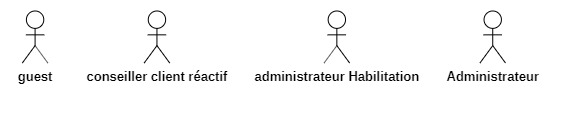
\includegraphics[width=0.7\linewidth]{img/conception/usecases/actors}
	\caption[Les acteurs de système]{Les acteurs de système}
	\label{fig:actors}
\end{figure}

La table \ref{tab:my-table} représente les tâches de chaque acteur de notre système.

\begin{longtable}[c]{|l|l|}
	\hline
	\rowcolor[HTML]{C0C0C0}
	Acteurs                      & Tâches                                                                                                                                                                                                                                                                                                                                                                                                                                                                                                                                                                                                                                                                                                                                                                                                                                                                                                                                                                                                                \\ \hline
	\endhead
	%
	Guest                        & \begin{tabular}[c]{@{}l@{}}\tabitem Consulter la page de simulation SRCD qui\\  permet de simuler l’inscription de client en\\ entrant à la boutique.\end{tabular}                                                                                                                                                                                                                                                                                                                                                                                                                                                                                                                                                                                                                                                                                                                                                                                                                                                             \\ \hline
	Conseiller client réactif    & \begin{tabular}[c]{@{}l@{}}\tabitem L’utilisation des PEF lors de l’ouverture de\\ fiche client pour utiliser une certaine\\ application telle que la consultation de\\ facture, gestion de la boite email\\ professionnelle, gestion des lignes\\ téléphoniques d’une entreprise, etc…\end{tabular}                                                                                                                                                                                                                                                                                                                                                                                                                                                                                                                                                                                                                                                                                                                                \\ \hline
	Administrateur Habilitations & \begin{tabular}[c]{@{}l@{}}\tabitem Gestion des utilisateurs(consultation, ajout,\\ modification, suppression, export, import et\\ recherche).\end{tabular}                                                                                                                                                                                                                                                                                                                                                                                                                                                                                                                                                                                                                                                                                                                                                                                                                                                                       \\ \hline
	Administrateur               & \begin{tabular}[c]{@{}l@{}}\tabitem Gestion des utilisateurs(consultation, ajout,\\ modification, suppression, export, import,\\ recherche, affectation aux boutiques, export\\ des affectations).\\ \tabitem Gestion des rôles(consultation, ajout,\\ modification, suppression et recherche).\\ \tabitem Consultation des données boutiques.\\ \tabitem Gestion des catégories des PEF(consultation,\\ ajout, modification, suppression et recherche).\\ \tabitem Gestion des PEF(consultation, ajout,\\ modification, suppression, recherche,\\ gestion des visibilités des PEF aux boutiques).\\ \tabitem Consultation des statistiques des logs des API\\ utilisées dans l’application.\\ \tabitem Consulter la page de simulation SRCD qui\\ permet de simuler l’inscription de client en\\ entrant à la boutique.\\ \tabitem L’utilisation des PEF lors de l’ouverture de fiche\\ client pour utiliser une certaine application\\ telle que la consultation de facture, gestion de\\ la boite email professionnelle, gestion des\\ lignes téléphoniques d’une entreprise, etc…\end{tabular} \\ \hline
	\captionsetup{justification=centering}
	\caption{Les tâches des acteurs de système}
	\label{tab:my-table}\\
\end{longtable}

\subsection[Les besoins fonctionnels]{Les besoins fonctionnels}
Notre application doit fournir un ensemble de fonctionnalités qui répondent aux exigences des acteurs. Les principales exigences fonctionnelles sont :
\begin{itemize}
	\item \textbf{Recevoir des rapports quotidiens des tests de non régression :} Chaque jour, les tests de non régression doivent être exécutés pour garantir que l'intégration de nouvelles fonctionnalités n'affecte pas le déroulement de notre système et envoyer un rapport complet aux personnes concernées.
	\item \textbf{Gestion les utilisateurs :} sert à ajouter, modifier, supprimer, consulter et rechercher les utilisateurs.
	\item \textbf{Gestion les rôles :} permet d'ajouter, modifier, supprimer, consulter et rechercher les rôles.
	\item \textbf{Consultation des données boutiques :} Consulter les informations des boutiques en détails.
	\item \textbf{Affectation des utilisateurs aux boutiques :} Affecter un utilisateur à une boutique, et par conséquence, cet utilisateur aura la possibilité d'accéder et utiliser les PEF de cette boutique. 
	\item \textbf{Gestion des catégories :} sert à ajouter, modifier, supprimer, consulter et rechercher les catégories.
	\item \textbf{Gestion des PEF :} L'administrateur peut gérer les PEF (ajouter, modifier, supprimer, consulter et rechercher).
	\item \textbf{Visibilité des PEF aux boutiques :} Donner l'autorisation aux boutiques pour utiliser un ensemble défini des PEF.
	\item \textbf{L’utilisation des PEF lors de l’ouverture de fiche client :} pour utiliser une certaine application telle que la consultation de facture, gestion de la boite email professionnelle, gestion des lignes téléphoniques d’une entreprise, etc. Les applications seront filtrés selon leur catégorie, le type de catégorie\footnote{Soit de type boutique ou de type centre d'appel} et de type d'utilisateur.
	\item \textbf{Simulation SRCD :} Simuler le mécanisme d'inscription de client en entrant à la boutique.
	\item \textbf{Consultation les logs des API :} Afficher des statistiques sur les requêtes des API et afficher les détails des causes des erreurs.
	\item \textbf{Traçabilité :} Tracer toutes actions prise lors de l'utilisation de Panoramix.
\end{itemize}
\subsection[Diagramme de cas d’utilisation global]{Diagramme de cas d’utilisation global}
Dans cette sous-section, nous exposons le diagramme de cas d’utilisation global qui permet de donner une vision globale du comportement fonctionnel de notre système.\\
La figure \ref{fig:usecasediagram-global} représente le diagramme de cas d’utilisation global.
\begin{figure}[H]
	\centering
	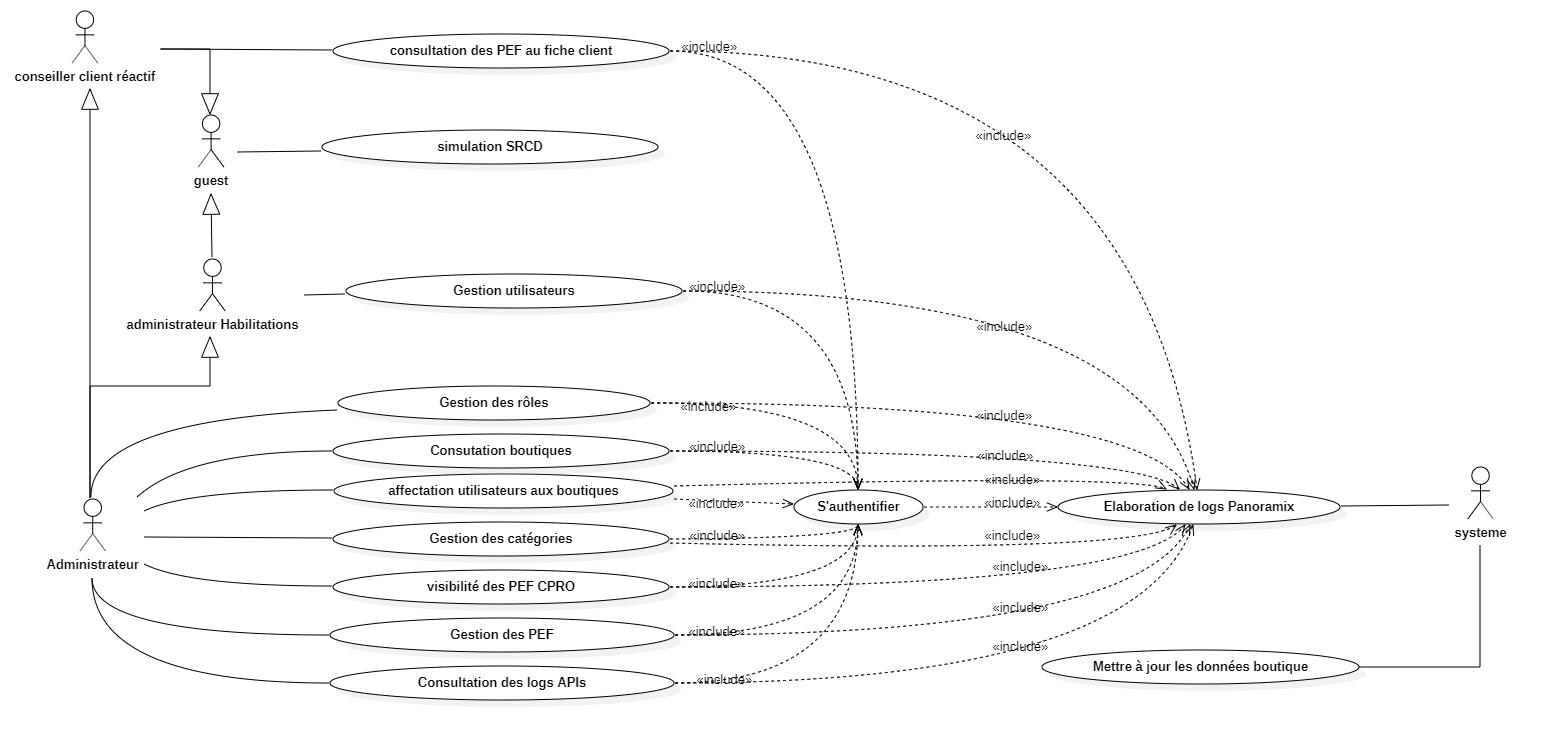
\includegraphics[width=1.1\linewidth]{img/conception/usecases/UseCaseDiagram-global}
	\caption[Diagramme de cas d'utilisation générale]{Diagramme de cas d'utilisation générale}
	\label{fig:usecasediagram-global}
\end{figure}
\subsection[Les besoins non fonctionnels]{Les besoins non fonctionnels}
Outre des besoins fonctionnels, le futur système doit également répondre aux contraintes suivantes :
\begin{itemize}
	\item \textbf{La rapidité de traitement :} Compte tenu du grand nombre de transactions par jour, le temps de traitement doit être le plus proche possible du temps réel.
	\item \textbf{La performance :} Nous utilisons les performances pour spécifier la durée pendant laquelle le système répond aux demandes d'entrée. Ce terme fait référence à la vitesse à laquelle le système effectue le traitement.
	\item \textbf{La disponibilité :} L'application devrait être opérationnelle d'une façon continue, car l’utilisateur peut faire des réservations à tout moment. Le système doit être en permanence à la disposition de ses utilisateurs.
	\item \textbf{Ergonomie et Simplicité :} Cette fonctionnalité permet à l’utilisateur d’être à l’aise lors de l’utilisation ou de la consultation du site.
	\item \textbf{L’extensibilité :} Cela nous donne la possibilité d’ajouter, de modifier ou de supprimer des fonctionnalités.
	\item \textbf{Fiabilité :} Notre application doit être bien testée avant de l’héberger aux clients à fin d’éviter les éventuels des bugs.
\end{itemize}

\section[Structure et découpage du projet]{Structure et découpage du projet}
Nous présentons, dans la suite, les différents intervenants dans notre projet ainsi que le cycle de vie de la méthode Scrum et nous finissons par la présentation de notre product backlog.
\subsection[Identification des rôles dans l’équipe SCRUM]{Identification des rôles dans l’équipe SCRUM}
Dans un projet SCRUM, l’équipe a un rôle fondamental : elle permet d’optimiser la productivité et la flexibilité. En effet, elle doit être auto-organisée et multifonctionnelle.\\
Le tableau \ref{tab:comp-scrum} représente la décomposition de l'équipe SCRUM de Panoramix\\
\begin{table}[H]
	\centering
	\begin{tabular}{|l|l|}
		\hline
		\rowcolor[HTML]{C0C0C0} 
		Nom \& prénom        & Rôle dans l'équipe   \\ \hline
		Nesrine ZIADIA       & Product owner        \\ \hline
		Meriem OUEDERNI      & Product owner Proxi. \\ \hline
		Mohamed Aymen FEKIRI & Scrum master         \\ \hline
		\begin{tabular}[c]{@{}l@{}}Nabila OUNI\\ Hichem BEN SAID\\ Lassad KEFI\end{tabular} & Développeurs \\ \hline
	\end{tabular}
	\captionsetup{justification=centering}
	\caption{Composition de l'équipe Scrum}
	\label{tab:comp-scrum}
\end{table}
\subsection[Planification d’un projet par Scrum]{Planification d’un projet par Scrum}
Pour appliquer correctement SCRUM, il faut comprendre le cycle de vie d’un sprint pendant un processus SCRUM. Le processus, illustré dans la figure \ref{fig:scrum}, est décrit ci-dessous : 
\begin{enumerate}[label=\arabic*.]
	\item Le Product owner crée le "product backlog" en identifiant et priorisant les user stories.
	\item Pendant la planification du sprint, l’équipe choisit un ensemble de " user stories " les plus prioritaires à partir du "product backlog" pour construire le sprint Backlog. 
	\item L’équipe implémente les "users stories " pendant une période qui dure de 2 à 4 semaines. 
	\item Durant le sprint, l’équipe se réunit chaque jour, "Daily Scrum", pour synchroniser les tâches. 
	\item À la fin du sprint, le travail doit être achevé pour faire une démonstration au client. 
	\item Le sprint est clôturé par un "sprint review" pour discuter les prochaines étapes du projet et par un "sprint rétrospectif" pour parler des manières à appliquer pour rendre l’équipe plus productive.
\end{enumerate}
\begin{figure}[H]
	\centering
	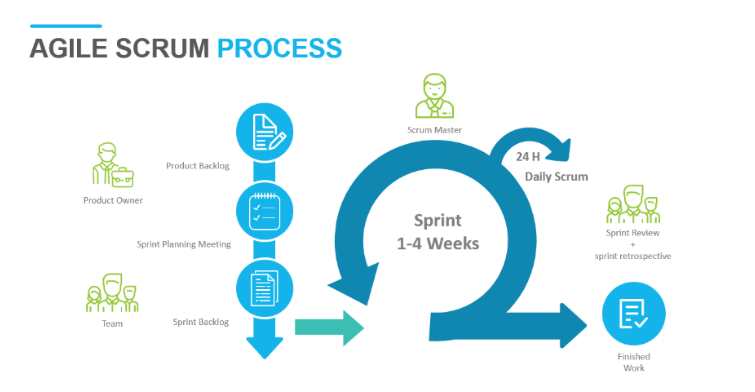
\includegraphics[width=0.9\linewidth]{img/scrum}
	\caption[Description de processus SCRUM]{Description de processus SCRUM}
	\label{fig:scrum}
\end{figure}
\subsection[Le Product Backlog du produit]{Le Product Backlog du produit}
Le backlog est élaboré avant le lancement des sprints, dans la phase de préparation. Il est utilisé pour la planification de la release, puis à chaque sprint, lors de la réunion de planification du sprint pour décider du sous-ensemble d’éléments. Les éléments y sont classés par priorité ce qui permet de définir l’ordre de réalisation.
La table \ref{tab:product-backlog} représente notre backlog de produit :
\begin{table}[H]
	\centering
	\resizebox{\textwidth}{!}{%
		\begin{tabular}{|l|c|c|}
			\hline
			\rowcolor[HTML]{C0C0C0} 
			Backlog du Produit & \multicolumn{1}{l|}{\cellcolor[HTML]{C0C0C0}priorité} & \multicolumn{1}{l|}{\cellcolor[HTML]{C0C0C0}Estimation} \\ \hline
			Migration de l’environnement \& automatisation des tests de non régression & 1 & Haute   \\ \hline
			Gestion des utilisateurs \& des rôles                                      & 2 & Haute   \\ \hline
			Intégration de module boutique \& affectation des utilisateurs aux boutiques   & 3 & Moyenne \\ \hline
			Gestion des catégories                                                         & 4 & Moyenne \\ \hline
			Gestion des PEF                                                            & 5 & Moyenne \\ \hline
			Simulation SRCD et consultation des logs API                               & 6 & faible  \\ \hline
			Elaboration des logs de l’application                                      & 7 & faible  \\ \hline
		\end{tabular}%
	}
    \captionsetup{justification=centering}
	\caption{Backlog de produit}
	\label{tab:product-backlog}
\end{table}

\subsection[Planification des sprints]{Planification des sprints}
Notre travail est divisé sur deux releases, le premier release contient la partie de migration de l’environnement, l’élaboration des tests de non régression et la gestion des utilisateurs et leurs rôles.\\
Le deuxième release contient la consultation des boutiques, l’affectation des utilisateurs, la gestion des PEF, la simulation SRCD et la consultation des logs.\\
\newpage
Le tableau \ref{tab:plan-sprints} montre la répartition des sprints relative à notre système.
\begin{table}[H]
	\centering
	\begin{tabular}{|l|l|l|}
		\hline
		\rowcolor[HTML]{9B9B9B} 
		\multicolumn{3}{|c|}{Répartition des sprints}                                           \\ \hline
		\rowcolor[HTML]{C0C0C0} 
		Les Releases & Les sprints               & Les tâches                                   \\ \hline
		\multirow{6}{*}{Release 1} & \multirow{4}{*}{Sprint 0} & Migration PHP                  \\ \cline{3-3} 
		&                           & Migration SGBD                               \\ \cline{3-3} 
		&                           & Migration Orange Framework \& Tools          \\ \cline{3-3} 
		&                           & Automatisation des tests de non régressions  \\ \cline{2-3} 
		& \multirow{2}{*}{Sprint 1} & Gestion des utilisateurs                     \\ \cline{3-3} 
		&                           & Gestion des rôles                            \\ \hline
		\multirow{9}{*}{Release 2} & \multirow{3}{*}{Sprint 2} & Intégration de module Boutique \\ \cline{3-3} 
		&                           & Affectation des utilisateurs aux boutiques   \\ \cline{3-3} 
		&                           & Simulation SRCD                              \\ \cline{2-3} 
		& \multirow{6}{*}{Sprint 3} & Gestion des catégories                       \\ \cline{3-3} 
		&                           & Gestion des PEF                              \\ \cline{3-3} 
		&                           & Visibilité des PEF à la boutique             \\ \cline{3-3} 
		&                           & Utilisation des PEF via la fiche client      \\ \cline{3-3} 
		&                           & Consultation des logs API                    \\ \cline{3-3} 
		&                           & Elaboration des logs d’application Panoramix \\ \hline
	\end{tabular}
	\captionsetup{justification=centering}
	\caption{Planification des sprints}
	\label{tab:plan-sprints}
\end{table}
\section[Environnement de travail]{Environnement de travail}
Dans cette partie, nous présenterons l’environnement de travail lors de la conception et la réalisation des tâches du projet.
\subsection[Environnement matériel]{Environnement matériel}
Lors de la réalisation de notre application, nous avons utilisé un seul ordinateur dont les configurations sont les suivants :
\begin{itemize}
	\item \textbf{PC} : DELL LATITUDE E5540
	\item \textbf{Processeur} : Intel i5-4210U
	\item \textbf{RAM} : 12 Go
	\item \textbf{Système d’exploitation} : Windows 10 Entreprise	
\end{itemize}
\subsection[Environnement de développement]{Environnement de développement}
\begin{itemize}
	\item \textbf{Eclipse \cite{eclipse} :} est un environnement de développement intégré (IDE) utilisé dans la programmation informatique. Il contient un espace de travail de base et un système de plugin extensible pour personnaliser l'environnement. Eclipse est principalement écrit en Java et son utilisation principale est le développement d'applications Java, mais il peut également être utilisé pour développer des applications dans d'autres langages de programmation via des plug-ins, notamment C, C++, C\#, JavaScript, PHP, Python et autres.

	\item \textbf{Visual studio Code \cite{vscode} :} est un éditeur de code redéfini et optimisé pour la création et le débogage d'applications web et cloud modernes. Visual Studio Code est gratuit et disponible sur votre plateforme favorite Linux, macOS et Windows.

	\item \textbf{Laragon \cite{laragon} :} est un environnement de développement universel, portable, isolé, rapide et puissant pour PHP, Node.js, Python, Java, Go, Ruby. Il est rapide, léger, facile à utiliser et facile à étendre. Laragon est idéal pour construire et gérer des applications web modernes. Il est axé sur la performance, conçu autour de la stabilité, de la simplicité, de la flexibilité et de la liberté.

	\item \textbf{Apache \cite{apache} :} Un serveur HTTP créé et maintenu sur la fondation d'Apache. Jusqu'en avril 2019, c'était le serveur HTTP le plus populaire sur le World Wide Web. Il est distribué sous les termes de la licence Apache.
	
	\item \textbf{MariaDB \cite{mariadb} :} est un système de gestion de base de données publié sous licence GPL. Il s'agit d'une branche communautaire de MySQL : la gouvernance du projet est assurée par la Fondation MariaDB, et sa maintenance est assurée par Monty Program AB, le créateur du projet.
	
	\item \textbf{HeidiSQL \cite{heidisql} :} est un outil de gestion de base de données avec éditeur SQL et générateur de requêtes. Il a été développé et optimisé pour une utilisation avec le SGBD relationnel MySQL/MariaDB.
\end{itemize}

\subsection[Environnement logiciel]{Environnement logiciel}
Dans cette partie, nous allons présenter les différents logiciels, framework et technologies web utilisés pour la réalisation des applications.
\begin{itemize}
	\item \textbf{SeleniumLibrary based on Python \cite{seleniumlib} :} est une bibliothèque de test web pour Robot Framework qui utilise l'outil Selenium en interne. SeleniumLibrary fonctionne avec Selenium 3 et 4. Elle supporte Python 2.7 ainsi que Python 3.6 ou plus récent. En plus de l'interpréteur Python normal, elle fonctionne également avec PyPy et Jython.

	\item \textbf{Robot Framework \cite{robotframework} :} est un framework d'automatisation basé sur Python et extensible par mot-clé pour les tests d'acceptation, le développement piloté par les tests d'acceptation, le développement piloté par le comportement et l'automatisation des processus robotiques. Il peut être utilisé dans des environnements distribués et hétérogènes, où l'automatisation nécessite l'utilisation de différentes technologies et interfaces. Le cadre est entouré d'un riche écosystème constitué de diverses bibliothèques et outils génériques qui sont développés dans le cadre de projets distincts.

	\item \textbf{Jenkins \cite{jenkins} :} est un outil d'intégration continue open source. Après les différends entre son auteur \textit{Kohsuke Kawaguchi} et Oracle, Jenkins devient une branche des outils Hudson. Jenkins est écrit en Java et il peut fonctionner dans un conteneur de servlet (comme Apache Tomcat), ou il peut être utilisé un serveur Web intégré en mode autonome.

	\item \textbf{GeckDriver \cite{geckodrive} :} est proxy pour l'utilisation de clients compatibles avec le W3C WebDriver pour interagir avec les navigateurs basés sur Gecko. Ce programme fournit l'API HTTP décrite par le protocole WebDriver pour communiquer avec les navigateurs Gecko, tels que Firefox. Il traduit les appels dans le protocole Marionnette à distance en agissant comme un proxy entre les extrémités locales et distantes.
	\item \textbf{Xvfb plugin \cite{xvfb} : } Xvfb ou X virtual framebuffer est un serveur d'affichage mettant en œuvre le protocole de serveur d'affichage X11. Contrairement aux autres serveurs d'affichage, Xvfb effectue toutes les opérations graphiques en mémoire sans afficher de sortie d'écran. C'est très utile si votre compilation nécessite un accès X11, par exemple pour effectuer des tests qui nécessitent une interface graphique.
	\item \textbf{Email Extension plugin \cite{emailextension} :} Ce plugin vous permet de configurer tous les aspects des notifications par courrier électronique. Vous pouvez personnaliser le moment où un courriel est envoyé, qui doit le recevoir et ce que le courriel dit.
	\item \textbf{Javascript \cite{js} :} est un langage de script utilisé pour créer et contrôler le contenu dynamique d'un site web, c'est-à-dire tout ce qui bouge, rafraîchit ou change de quelque manière que ce soit sur votre écran sans vous obliger à recharger manuellement une page web. Des choses comme : des graphiques animés, des diaporamas de photos, des suggestions de texte à remplir automatiquement, des formulaires interactifs.
	
	\item \textbf{jQuery \cite{jquery} :} est une bibliothèque JavaScript multi-plateforme gratuite, qui a été créée pour faciliter l'écriture de scripts côté clients avec du code HTML sur les pages Web.
	
	\item \textbf{Axios \cite{axios} :} est un client HTTP populaire, basé sur la promesse, qui comporte une API facile à utiliser et peut être utilisé à la fois dans le navigateur et dans Node.js. Effectuer des requêtes HTTP pour récupérer ou enregistrer des données est l'une des tâches les plus courantes qu'une application JavaScript côté client devra effectuer.
	
	\textbf{HTML5 \cite{html} :} est un langage de balisage utilisé pour structurer et présenter le contenu sur le World Wide Web. Elle est la dernière révision majeure d'HTML. HTML5 spécifie deux syntaxes pour le modèle abstrait défini par le DOM : HTML5 et XHTML5.
	
	\item \textbf{PHP \cite{php} :} préprocesseur hypertexte, connu sous son acronyme PHP, est un "langage de programmation" gratuit qui est principalement utilisé pour générer des pages Web dynamiques via un serveur HTTP, mais il peut également fonctionner comme n'importe quel langage interprété localement. PHP est un langage impératif orienté.
	
	\item \textbf{Orange Framework \& Tools \cite{oft} :} est un squelette d'application PHP/MySQL prêt-à-l'emploi. Ce framework PHP est sécurisé et équipé d'outils de sécurité pour accompagner les développements, charté et respectueux de l'identité du Groupe \#Boosted, performant et compatible avec toutes les offres d'hébergement \#12factor, souple et adapté à la construction d'interfaces REST et HTML, équipé d'outils pour accélérer les développements et gérer les spécificités d'Orange et adapté aux débutants comme aux experts.\\
	L'OFT est surtout un framework basé sur Symfony et Zend PHP, produit de réflexions sur ce qui est jugé le plus pertinent pour les projets du Groupe Orange puisqu'il est taillé selon les besoins de la communauté PHP d'Orange et qui suit les standards et réutilise les composants reconnus.
	
	\item \textbf{Boosted \cite{boosted} :} est représenté comme la bibliothèque HTML, CSS et JS d'Orange basée sur Bootstrap 4.5.0, la boîte à outils open source frontale la plus populaire au monde.
	
\end{itemize}

\section[L'architecture de la solution]{L'architecture de la solution}
Dans cette partie, nous présenterons l'architecture logicielle et matérielle utilisée lors du développement de notre application.
\subsection[L'architecture logique]{L'architecture logique}
\subsubsection{L'architecture logique des tests de non régression}
Les tests de non régression permettent de valider que la mise en ligne d’une nouvelle fonctionnalité sur un logiciel n’impactera pas les fonctions déjà existantes. Ces tests ont pour but de s’assurer que les modifications et évolutions effectuées par les développeurs lors du dernier sprint n’ont pas entraîné d’effet de bord, en altérant les parties du code non modifiées.\newpage
Nous présentons dans ce qui est suit l'enchaînement des tests de non régression de notre application. La figure \ref{fig:jenkins-schema} illustre la procédure des tests.
\begin{figure}[H]
	\centering
	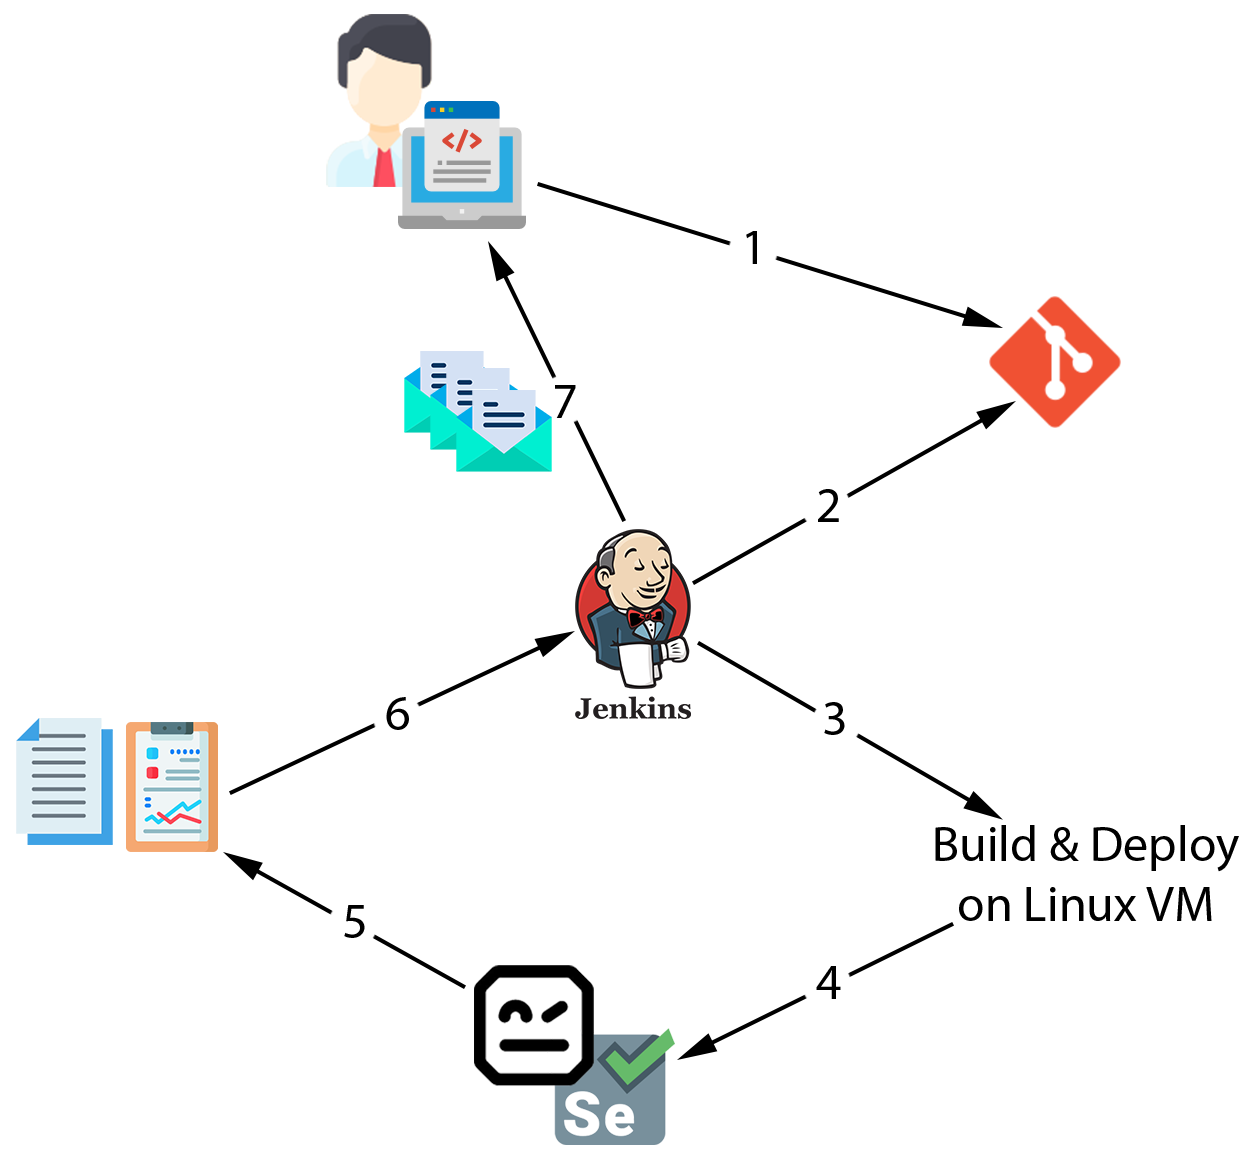
\includegraphics[width=0.5\linewidth]{img/jenkins}
	\caption[L'architecture logique des tests de non régression]{L'architecture logique des tests de non régression}
	\label{fig:jenkins-schema}
\end{figure}
\begin{enumerate}
	\item[Étape 1 -] Le développeur de l’équipe Panoramix fait un « push » de code de robot Framework vers le repo git de « Orange Forge ».
	\item[Étape 2 et 3 -] Jenkins va cloner ce repo dans une VM Linux et prépare l’environnement pour lancer les tests.
	\item[Étape 4 -] les 54 tests de non régression s’exécutent test par test et chaque test simule un scénario d’utilisation de notre portail.
	\item[Étape 5 -] À la fin des tests, Robot Framework génère 3 fichiers dont le fichier report.html et log.html sont les plus importants :
	\begin{itemize}
		\item\textbf{ Log.html :} Les fichiers journaux contiennent des détails sur les cas de tests exécutés au format HTML. Ils ont une structure hiérarchique indiquant la suite de tests, le scénario de test et les détails des mots-clés. Les fichiers journaux sont nécessaires presque à chaque fois que les résultats des tests doivent être examinés en détail. Même si les fichiers journaux contiennent également des statistiques, les rapports sont plus utiles pour obtenir une vue d'ensemble de haut niveau.
		\item \textbf{Report.html :} Les fichiers de rapport contiennent un aperçu des résultats de l'exécution des tests au format HTML. Ils contiennent des statistiques basées sur les balises et les suites de tests exécutés, ainsi qu'une liste de tous les cas de tests exécutés. Lorsque les rapports et les journaux sont générés, le rapport comporte des liens vers le fichier journal pour faciliter la navigation vers des informations plus détaillées. Il est facile de voir l'état général de l'exécution des tests à partir du rapport, car sa couleur de fond est verte, si tous les tests critiques réussissent, et rouge vif dans le cas contraire.
	\end{itemize}
	\item[Étape 6 et 7 -]  Jenkins récupère les fichiers générés par robot Framework et les envoyer en email vers les personnes concernées.
\end{enumerate}
\newpage
\subsubsection{L'architecture logique de l’application}
Dans notre application, nous envisageons d’utiliser une architecture 3-tiers qui sera réparti en trois couches comme suit :
\begin{itemize}
	\item\textbf{ Couche 1 (Site) :} Cette couche contient les interfaces côté utilisateurs qui interagissent souvent avec l’application Panoramix.
	\item\textbf{ Couche 2 (Serveur) : }Cette couche représente la partie de traitement qui contient toutes nos APIs, cette partie sera réalisée avec Apache qui est un serveur HTTP.
	\item \textbf{Couche 3 (Base de Données) :} Cette couche représente le côté base de données de notre site qui sera une base de données MySQL.
\end{itemize}
\begin{figure}[H]
	\centering
	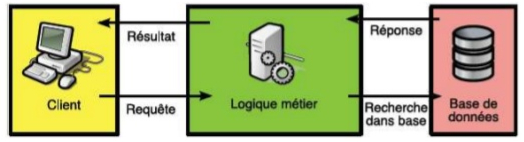
\includegraphics[width=0.7\linewidth]{img/architectures-3tiers-web}
	\caption[L'architectures 3 tiers du Web]{L'architecture 3 tiers du Web}
	\label{fig:architectures-3tiers-web}
\end{figure}

\subsection[L'architecture logicielle]{L'architecture logicielle}
\subsubsection{L'architecture logicielle des tests de non régression}
Les tests de non régression sont divisés en 3 grandes parties :
\begin{itemize}
	\item Configuration globale : un dossier qui contient un fichier de configurations globales nécessaires dans la plupart des tests.
	\item Les fonctions globales : ce dossier contient un fichier des fonctions générales utilisées dans tous les tests.
	\item TestSuite : un dossier contient tous les tests de non régression. Chaque test est divisé en 3 parties :
		\subitem • Fichier.robot : le script de test à exécuter.
		\subitem • Config : est un dossier contient les configurations nécessaires pour ce test.
		\subitem • Fonctions : est un dossier contient les fonctions nécessaires pour ce test.
\end{itemize}
\subsubsection{L'architecture  logicielle de l’application}
L’organisation du code source est assuré par le biais du modèle MVC. Mais son rôle est principalement de segmenter la logique du code en trois parties. 
\begin{itemize}
	\item Modèle(M) : Permet de récupérer des données brutes stockées dans notre base de données.
	\item Vue(V) : Cette partie inclut juste les fichiers html et CSS, mais aussi quelques boucles et conditions PHP très simples qui se focalisent sur l’affichage. 
	\item Contrôleur(C) : Ce dernier est assimilable à une passerelle entre les vues et le modèle. Il contient exclusivement que du PHP et gère notamment les droits d’accès de chaque utilisateur. 
\end{itemize}\newpage
La figure \ref{fig:mvc} schématise l’échange d’informations entre les éléments de l’architecture MVC
\begin{figure}[H]
	\centering
	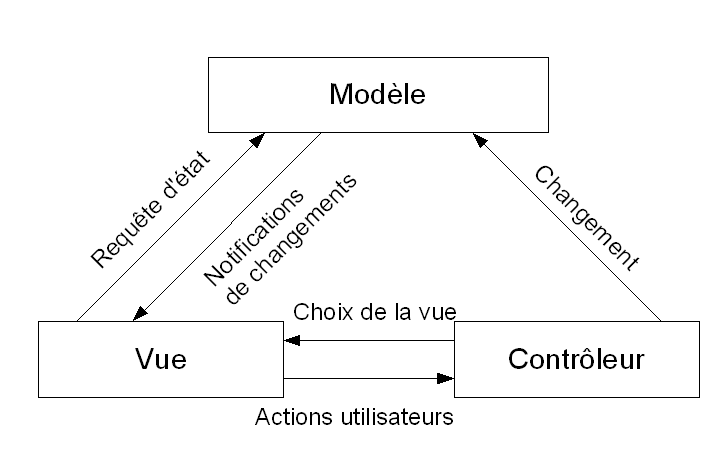
\includegraphics[width=0.7\linewidth]{img/mvc}
	\caption[L'architecture logicielle de l’application]{L'architecture logicielle de l’application}
	\label{fig:mvc}
\end{figure}

\section*{Conclusion}
Dans ce chapitre, nous avons présenté les différents concepts nécessaires à la compréhension du projet. Nous avons également identifié les besoins fonctionnels, non fonctionnels ainsi que les acteurs. Par la suite, nous avons réalisé une conception pour notre projet, présenté l’environnement de travail et l’architecture de la solution. Dans le chapitre suivant nous entamons le développement du premier release.
        \clearpage
        
        \chapter{Sprint 0 – Migration de Panoramix}

\section*{Introduction}
Après avoir analyser et spécifier les besoins globaux de notre client, nous détaillerons les différentes étapes effectuées durant ce premier sprint ayant pour objectif « la migration de notre application ».  Cette migration assure la possibilité d’intégrer la nouvelle partie dans Panoramix.\\
Nous commencerons, tout d’abord, par présenter le backlog du sprint suivi d’une analyse détaillée et une comparaison entre les outils.

\section[Sprint Backlog]{Sprint Backlog}
Le tableau \ref{tab:sprint-backlog-sprint0}, qui représente une liste de tâches exprimées sous forme de besoins, illustre la liste des tâches de notre backlog de sprint
\begin{table}[H]
	\centering
	\begin{tabular}{|l|l|}
		\hline
		\rowcolor[HTML]{C0C0C0} 
		Exigences & Sous tâches                           \\ \hline
		1.1      & Migration de PHP 5.6 vers PHP 7.2    \\ \hline
		1.2      & Migration de MySQL vers MariaDB      \\ \hline
		1.3      & Migration de OFT2.2 vers OFT3        \\ \hline
		1.4      & Automatisation des tests de non régression \\ \hline
	\end{tabular}
	\captionsetup{justification=centering}
	\caption{Sprint backlog de sprint 0}
	\label{tab:sprint-backlog-sprint0}
\end{table}

\section[Migration de PHP 5.6 vers PHP 7.2]{Migration de PHP 5.6 vers PHP 7.2}
Dans cette section, nous comparons les critères le plus intéressants pour notre projet telque la performance, traitement des exceptions et le support de 64 bits entre les deux versions de PHP : version actuelle php5.3 et la version cible php7.2.

\subsection[Performance]{Performance}
Les performances de PHP 7 sont bien meilleures que celles de PHP 5. PHP 4 utilise le moteur Zend et PHP 5 utilise le moteur Zend II. Cependant, avec PHP 7, vient un tout nouveau moteur appelé PHPNG. Le "NG" signifie "Next Generation". Le moteur PHPNG améliore les performances du double avec une utilisation optimisée de la mémoire.
\begin{table}[H]
	\centering
	\begin{tabular}{l|l|l|}
		\cline{2-3}
		& \cellcolor[HTML]{C0C0C0}PHP5.3 & \cellcolor[HTML]{C0C0C0}PHP7.2 \\ \hline
		\multicolumn{1}{|l|}{\cellcolor[HTML]{C0C0C0}consommation de mémoire (Mo)}    & 7.8                            & 3.58 (-46\%)                   \\ \hline
		\multicolumn{1}{|l|}{\cellcolor[HTML]{C0C0C0}temps d'exécution CPU (seconde)} & 0.8                            & 0.35 (-44\%)                   \\ \hline
	\end{tabular}
\captionsetup{justification=centering}
	\caption{Comparaison de performance entre PHP 5.6 et PHP 7.2 sur le site journaldunet.com }
	\label{tab:perf-php}
\end{table}
\subsection[Traitement des exceptions]{Traitement des exceptions}
Le traitement des erreurs fatales dans le PHP 5 est assez compliqué. Le PHP 7 a remplacé plusieurs erreurs majeures avec des exceptions qui peuvent être traitées facilement. Cela est dû à l'introduction des nouveaux objets d'exception du moteur. 
\subsection[Support de 64 bits ]{Support de 64 bits }
PHP 5 ne prend pas en charge les entiers 64 bits ni les fichiers volumineux, alors que le PHP 7 supporte le 64 bits, ce qui permet d'utiliser des entiers 64 bits natifs et des fichiers volumineux.
\section[Migration de MySQL vers MariaDB]{Migration de MySQL vers MariaDB}
Dans cette partie du rapport, nous comparons le système de gestion de base de données actuel et le système de gestion de base de données cible. Nous examinerons les aspects liés aux performances, à la sécurité et aux principales caractéristiques, et nous énumérerons tous les aspects à prendre en compte avant de choisir la base de données qui répondra à nos besoins.
\subsection{Plus d'options pour les moteurs de stockage}
 y a 12 nouveaux moteurs de stockage intégrés dans MariaDB. Parmi ceux-ci, on trouve CONNECT, Spider et SphinxSE. Visitez leur page Moteurs de stockage pour une liste complète de ces moteurs, comment ils fonctionnent et comment les exploiter pour optimiser votre base de données.
\subsection{Améliorations de la vitesse}
MariaDB présente de nombreuses nouvelles améliorations de vitesse par rapport à MySQL standard. Ces performances améliorées permettent à MariaDB de se différencier des performances de base des serveurs MySQL traditionnels. Comme MySQL, MariaDB possède des dizaines de fonctionnalités pour l'optimisation de la vitesse, y compris l'accès au disque, les améliorations de JOIN et EXPLAIN, la sous-requête, les tables/vues dérivées, le contrôle de l'exécution et le contrôle de l'optimiseur.
\subsection{Indexes/Cache plus rapides}
En utilisant le moteur de stockage MEMORY, MariaDB peut compléter les instructions INSERT jusqu'à 24\% plus vite que les serveurs MySQL traditionnels, avec CHECKSUM TABLE et MyISAM Segment Key Cache étant 4x plus rapide.
\subsection{Un pool de connexion plus rapide et plus grand}
MariaDB bénéficie d'un pool de threads amélioré qui fonctionne plus rapide et prend en charge plus de 200 000 connexions là où MySQL standard ne supporte pas ce nombre.
\subsection{Réplication améliorée}
MariaDB bénéficie d'une réplication plus rapide et plus sûre, les mises à jour étant jusqu'à 2 fois plus rapides qu'avec les configurations de réplication MySQL traditionnelles. Désormais possible, la réplication parallèle assure l'existence de configurations Active/Active ou Master/Master. La réplication de MariaDB est rétrocompatible avec les serveurs MySQL, de sorte que la migration de votre cluster vers MariaDB est possible en utilisant un nœud à la fois.
\subsection{Nouvelles extensions/caractéristiques}
Il y a plusieurs nouvelles extensions et fonctionnalités, pour en nommer quelques-unes, les déclarations WITH, JSON et KILL. DECIMAL augmente de 30 à 38 décimales, tandis que KILL ALL permet d'effectuer des requêtes pour un utilisateur spécifique.
\subsection{Liste des fonctionnalités et la documentation}
Le site web MariaDB disponible présente une liste complète d'améliorations et de fonctionnalités, ainsi qu’une documentation bien détaillée.
\section{Migration d’OFT2 vers OFT3}
Dans cette section, nous présentons l’outil principal de développement de notre application OFT ( Orange Framework \& Tools ) et nous comparons les deux versions : version actuelle 2.2 et la version cible 3.
\subsection{Points forts d’OFT 3}
Parmi les principales raisons de migration, le support de PHP 7 d’où les versions précédentes  d’OFT ne sont pas compatibles avec PHP7. Un autre atout pour notre projet est la redirection simple des sorties des logs. En plus, les dépendances du framework ont été mises à jour et la performance de la framework est améliorée comme l'illustre la figure suivante :
\begin{figure}[H]
	\centering
	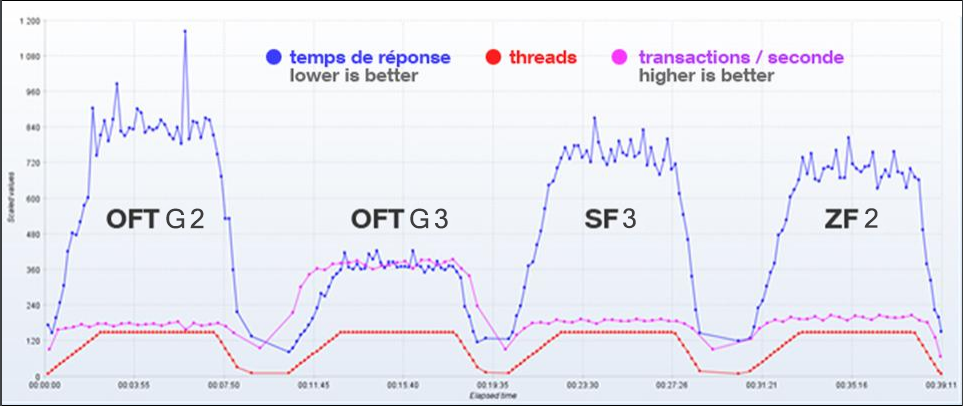
\includegraphics[width=0.7\linewidth]{img/oft-3}
	\caption[Comparaison performance entre OFT2 et OFT3]{Comparaison performance entre OFT2 et OFT3}
	\label{fig:oft-3}
\end{figure}
\section[Automatisation des tests de non régression]{Automatisation des tests de non régression}
Dans cette section, nous présentons la réalisation des différentes étapes d’automatisation des tests de non régression indiquées dans la figure \ref{fig:jenkins-schema} ci-dessus.
\subsection{Objectifs des tests}
Notre application Panoramix est considérée comme un portail qui assure l’accès aux différents PEFs ( points d’entrée fonctionnels ). Pour cela, l’équipe Panoramix décide de développer des  tests de non régression ou autrement des tests de l’IHM sur l’application de serveur d'intégration pour vérifier l’accès aux PEFs avec d’intégrer les modifications de code dans le serveur de production.
\subsection{Objectifs des tests}
Notre application Panoramix est considérée comme un portail qui assure l’accès aux différents PEFs ( points d’entrée fonctionnels ). Pour cela, l’équipe Panoramix décide de développer des  tests de non régression ou autrement des tests de l’IHM sur l’application de serveur d'intégration pour vérifier l’accès aux PEFs avec d’intégrer les modifications de code dans le serveur de production.
\subsection{Définition des tests}
Les tests sont envoyés sous format un fichier Excel contient :
\begin{itemize}
	\item Code de test : indique l’identifiant de chaque test
	\item fonctionnalité : indique une courte description de test
	\item jeu de données : cette colonne contient les valeurs de variables à utiliser
	\item Cas de gestion : précise la motif lors le test
	\item Etapes : représentent le scénario d'exécution de test
	\item Résultat attendu : précise le résultat de l’IHM après l'exécution de notre scénario  
	\item Ecrans : Capture d’écran de résultat attendu 
	\item Commentaire : Cette colonne est réservée aux commentaires supplémentaires ou une indication.
\end{itemize}
Nos 54 tests peuvent être présentés comme illustre la figure suivante :
\begin{figure}[H]
	\centering
	\includegraphics[width=1\linewidth]{"img/excel robot"}
	\caption[Fichier de description des tests]{Fichier de description des tests}
	\label{fig:excel-robot}
\end{figure}
\subsection{Réalisation}
Lors de cette partie, nous présenterons les différentes étapes de réalisation en spécifiant les étapes de configuration de Jenkins.\newpage
\subsubsection{Création de projet Jenkins}
Commençant tout d’abord par la création d’un projet Jenkins
\begin{figure}[H]
	\centering
	\includegraphics[width=0.9\linewidth]{"img/jenkins/creation projet"}
	\caption[Création de projet Jenkins]{Création de projet Jenkins}
	\label{fig:creation-projet}
\end{figure}

\subsubsection{Configuration du plugins}
Le projet est maintenant prêt, nous préparons les configurations nécessaires pour l'exécution des tests Cases de Robot Framework tels que les configurations du plugins :
\begin{itemize}
	\item \textbf{Xvfb plugin }
	\begin{figure}[H]
		\centering
		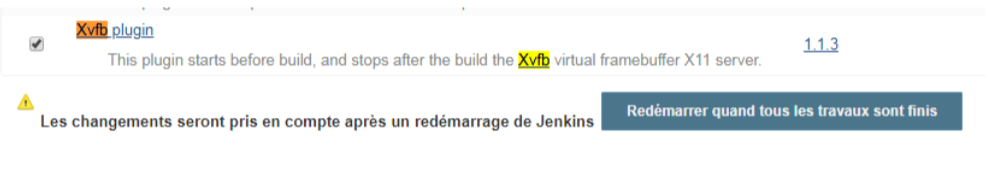
\includegraphics[width=0.9\linewidth]{img/jenkins/xvfb}
		\caption[plugin Xvfb]{plugin Xvfb}
		\label{fig:xvfb}
	\end{figure}
	
	\item \textbf{Email Extension}
	\begin{figure}[H]
		\centering
		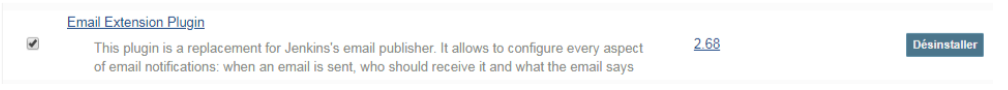
\includegraphics[width=0.9\linewidth]{img/jenkins/email}
		\caption[Email Extension plugin]{Email Extension plugin}
		\label{fig:email}
	\end{figure}
	
\end{itemize}
\newpage
et la configuration de l'environnement de build :
\begin{itemize}
	\item GeckoDrive
	\item Firefox
	\item Robot Framework
\end{itemize}
\begin{figure}[H]
	\centering
	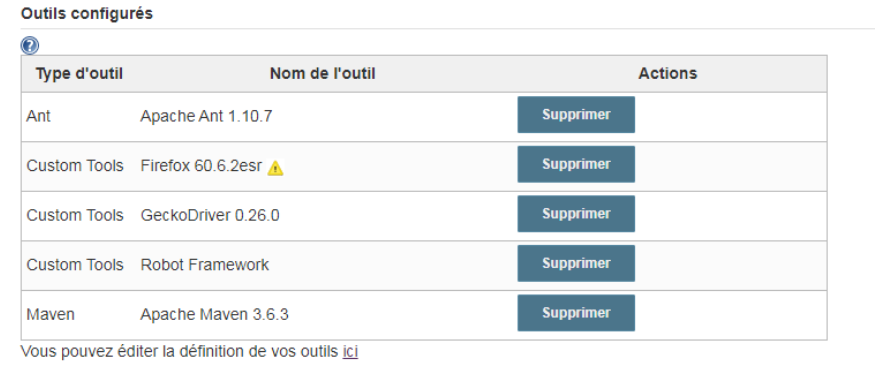
\includegraphics[width=0.7\linewidth]{img/jenkins/env-build}
	\caption[La configuration de l'environnement de build]{La configuration de l'environnement de build}
	\label{fig:env-build}
\end{figure}
\subsection{Gestion de code source}
Dans cette partie, nous configurons Jenkins de façon à récupérer les tests cases de Robot Framework. Nous choisissons la gestion de code avec Git et nous déclarons les dépôts distants hébergé chez Orange Forge avec la branche /develop. Chaque projet Jenkins possède un dépôt distant pour importer les tests. Lorsque le job est exécuté, Jenkins s’assure à chaque fois d’importer la dernière version des tests. Pour la configuration, il suffit de renseigner l’URL https de dépôts distants et fournir le nom d’utilisateur et le mot de passe. Un champ nous permet aussi de spécifier la branche du dépôt à utiliser comme l'illustre la figure suivante
\begin{figure}[H]
	\centering
	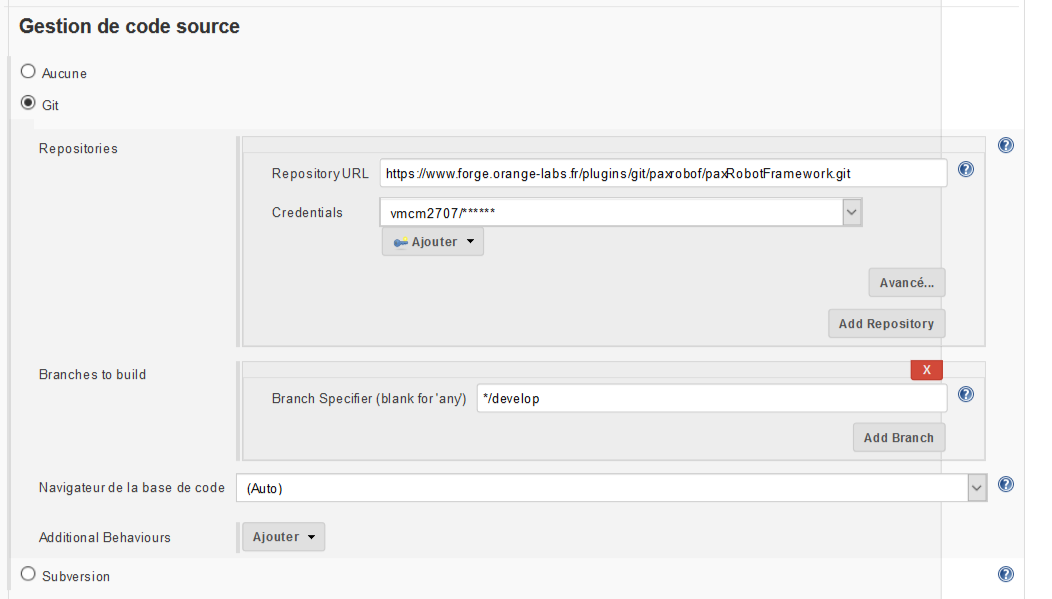
\includegraphics[width=0.7\linewidth]{img/jenkins/source}
	\caption[Gestion de source sous Jenkins]{Gestion de source sous Jenkins}
	\label{fig:source-jenkins}
\end{figure}

\subsection{Déclenchement de build }
Dans cette étape nous configurons la façon avec laquelle le job est lancé, plusieurs choix sont disponibles : soit périodiquement, soit par un déclencheur manuel.\\
Pour le premier choix, nous configurons la section “Ce qui déclenche le build” dans la configuration de job pour assurer que le build s'exécute de lundi à vendredi à 07:30 du matin.
\begin{figure}[H]
	\centering
	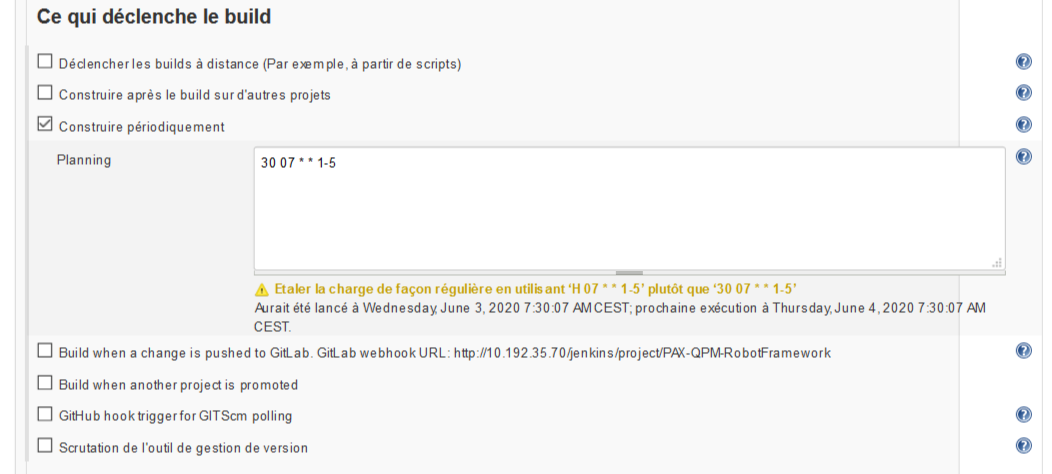
\includegraphics[width=0.8\linewidth]{img/jenkins/declanchement}
	\caption[Déclanchement de job Jenkins]{Déclanchement de job Jenkins}
	\label{fig:declanchement}
\end{figure}

\subsection{L’environnement de build}
\subsubsection{Build}
Dans cette étape, nous précisons l’action principale du job. Pour le job de tests, nous invoquons robot framework pour exécuter tous les tests cases dans le repo. Jenkins nous offre la possibilité de spécifier le chemin du test ainsi que le fichier robot. La figure présente notre configuration de déploiement.
\begin{figure}[H]
	\centering
	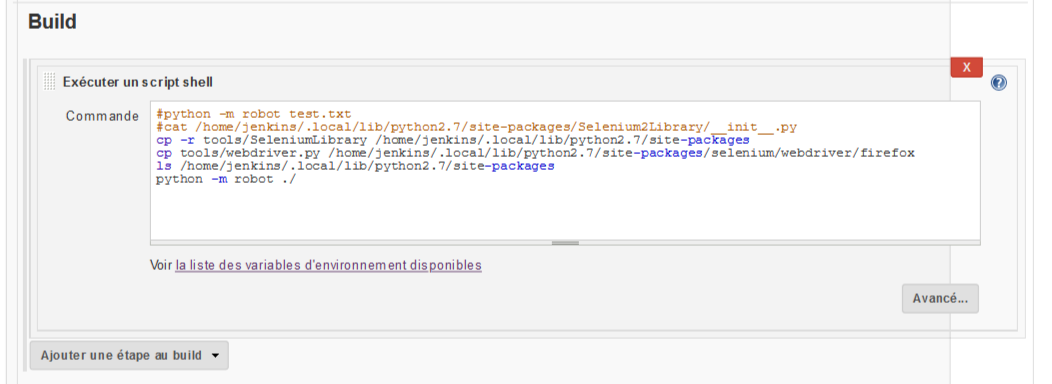
\includegraphics[width=0.8\linewidth]{img/jenkins/build}
	\caption[Build de job Jenkins]{Build de job Jenkins}
	\label{fig:build}
\end{figure}

\subsubsection{Actions à la suite du build}
Dans cette étape, nous activons la notification par mail, en attachant les  deux fichiers report.html et log.html, présenté par la figure suivante :
\begin{figure}[H]
	\centering
	\includegraphics[width=1\linewidth]{"img/jenkins/actions after"}
	\caption[Actions à la suite du build de job Jenkins]{Actions à la suite du build de job Jenkins}
	\label{fig:actions-after}
\end{figure}
\newpage
\subsection{Exécution de job}
Dans cette partie, nous présentons l’exécution du job. Jenkins offre la possibilité d’avoir une sortie console pour les commandes qu’il exécute.\\
La figure suivante représente la sortie de tous les outils du pipeline, ceci permet de garder une trace de l’exécution du job.
\begin{figure}[H]
	\centering
	\includegraphics[width=1\linewidth]{"img/jenkins/exemple console"}
	\caption[Extrait de sortie de console]{Extrait de sortie de console}
	\label{fig:exemple-console}
\end{figure}
l’exécution de robot framework génère deux fichiers qui résument les résultats de tests en basant sur des éléments graphiques facilitant la compréhension et la navigation.
\begin{itemize}
	\item Fichier report.html
	\begin{figure}[H]
		\centering
		\includegraphics[width=0.55\linewidth]{"img/jenkins/exemple report"}
		\caption[Extrait de rapport Jenkins]{Extrait de rapport Jenkins}
		\label{fig:exemple-report}
	\end{figure}
	\item Fichier log.html
	\begin{figure}[H]
		\centering
		\includegraphics[width=0.55\linewidth]{"img/jenkins/exemple log"}
		\caption[Extrait de log Jenkins]{Extrait de log Jenkins}
		\label{fig:exemple-log}
	\end{figure}
\end{itemize}

\section*{Conclusion}
Dans ce chapitre de sprint 0, nous avons migré notre application vers l’environnement souhaité et nous avons développé les tests et nous avons automatisé les tests sur jenkins.Dans le chapitre suivant, nous entamons de terminer la release 1 avec le sprint 1.




        \clearpage
        
        % !TeX spellcheck = fr_FR
\chapter{Sprint 1 – Gestion des utilisateurs et les rôles}
	
\section*{Introduction}
Ce chapitre fait l’objet d’une présentation du deuxième sprint du projet. Ce dernier comporte la gestion des utilisateurs et leurs rôles.
Tout d'abord, nous allons commencer par la description de le sprint backlog et les user stories. Ensuite, nous allons exprimer ces user stories en diagrammes de conception. Enfin, nous présenterons le travail réalisé et les résultats obtenus.
\section[Sprint Backlog]{Sprint Backlog}
Le sprint Backlog permet de faciliter la récupération des tâches et qui fait la mise au point du travail tout en précisant les tâches. Ces dernières contiennent tous les user-stories du Product Backlog.
\subsection[But du sprint]{But du sprint}
La première règle à suivre avant de se lancer dans un sprint, l’équipe SCRUM doit obligatoirement définir le but de ce sprint. Et pour cela, nous devons répondre à une question existentielle: Pourquoi faisons-nous ce sprint?\\
Donc, suite à une conversation entre le Product Owner et l’équipe SCRUM, nous avons conclu que le but de notre premier sprint sera : «Gestion des utilisateurs et leurs rôles».
\subsection[User stories]{User stories}
Après avoir déterminé l'objectif exact du sprint, il est temps de déterminer les user stories que nous voulons y inclure. Lors de la sélection de ces user stories, nous devons garder à l'esprit la priorité de chaque user story que nous avons configurée lorsque nous avons établi notre backlog produit.
\begin{longtable}[c]{|l|l|l|}
	\hline
	\rowcolor[HTML]{C0C0C0} 
	User stories &
	Tâches &
	Complexité\footnotemark{}\\ \hline
	\endhead
	%
	\begin{tabular}[c]{@{}l@{}}En tant qu’un \\ administrateur/admin.\\  habilitations, je souhaite de gérer \\ les utilisateurs de Panoramix\end{tabular} &
	\begin{tabular}[c]{@{}l@{}}Ajouter les interfaces de la gestion\\  des utilisateurs\\ \tabitem Consultation\\ \tabitem Modification\\ \tabitem Suppression\\ \tabitem Création \\ \tabitem Recherche\\ et la logique derrière\end{tabular} &
	1 \\ \hline
	\begin{tabular}[c]{@{}l@{}}En tant qu’un \\ administrateur/admin.\\  habilitations, je souhaite\\  d’importer(ADD) ou supprimer \\ (DEL) des utilisateurs à partir d'un\\ fichier csv\end{tabular} &
	\begin{tabular}[c]{@{}l@{}}Ajouter bouton “importer” dans \\ l’interface de gestion des\\  utilisateurs et la logique derrière \\ en fonction de structure de le \\ fichier csv\end{tabular} &
	2 \\ \hline
	\begin{tabular}[c]{@{}l@{}}En tant qu’un \\ administrateur/admin. \\ habilitations, je souhaite\\ d’exporter les informations des \\ utilisateurs dans un fichier csv\end{tabular} &
	\begin{tabular}[c]{@{}l@{}}Ajouter bouton “exporter” dans\\ l’interface de gestion des \\ utilisateurs et la logique derrière\end{tabular} &
	2 \\ \hline
	\begin{tabular}[c]{@{}l@{}}En tant qu’un administrateur, je \\ souhaite de gérer les rôles\end{tabular} &
	\begin{tabular}[c]{@{}l@{}}Ajouter les interfaces de la gestion\\  des rôles\\ \tabitem Consultation\\ \tabitem Modification\\ \tabitem Suppression\\ \tabitem Création\\ \tabitem Recherche\\ et la logique derrière\end{tabular} &
	1 \\ \hline
	\begin{tabular}[c]{@{}l@{}}En tant qu’un administrateur, je\\  souhaite de gérer les types de rôles\end{tabular} &
	\begin{tabular}[c]{@{}l@{}}Ajouter les interfaces de la gestion \\ des types de rôles\\ \tabitem Consultation des types de rôles.\\ \tabitem Attribution de types au rôle\\ \tabitem Modification de types\\ \tabitem Suppression de l’attribution\\ \tabitem Recherche \\ et la logique derrière\end{tabular} &
	2 \\ \hline
	\begin{tabular}[c]{@{}l@{}}En tant qu’un administrateur, je\\  souhaite d’activer/désactiver le \\ rôles attribué à un utilisateur\end{tabular} &
	\begin{tabular}[c]{@{}l@{}}Ajouter les interfaces de la \\ gestion des rôles\\ \tabitem Consultation\\ \tabitem Modification\\ \tabitem  Recherche\\ et la logique derrière\end{tabular} &
	2 \\ \hline
	\captionsetup{justification=centering}
	\caption{user stories sprint 1}
	\label{tab:user-stories-sprint1}\\
\end{longtable}
\footnotetext{plus faible plus complexe}

\section{Etude et réalisation du sprint 1}
La deuxième partie de notre projet, qui représente le module de gestion des utilisateurs et leurs rôles, nous donne la possibilité d’ajouter la nouvelle population CPRO.
\subsection{Diagramme de cas d’utilisation global sprint 1}
La figure \ref{fig:usecase-sprint1} décrit le diagramme de cas d’utilisation global du sprint 1.
\begin{figure}[H]
	\centering
	\includegraphics[width=0.7\linewidth]{"img/conception/usecases/sprint 1/usecase-Sprint1"}
	\caption[Diagramme de cas d’utilisation global sprint 1]{Diagramme de cas d’utilisation global sprint 1}
	\label{fig:usecase-sprint1}
\end{figure}
\subsection{Raffinement et description textuelle des diagrammes de cas d’utilisation}
Dans cette section, nous présentons les diagrammes des cas d’utilisation détaillés et leurs descriptions textuelles.
\subsubsection{Cas d’utilisation «Gérer utilisateurs»}
La figure \ref{fig:usecase-gestion-users} décrit le raffinement du cas d’utilisation « Gérer utilisateurs »
\begin{figure}[H]
	\centering
	\includegraphics[width=1\linewidth]{"img/conception/usecases/sprint 1/usecase-gestion-users"}
	\caption[Cas d’utilisation «Gérer utilisateurs»]{Diagramme ce cas d’utilisation «Gérer utilisateurs»}
	\label{fig:usecase-gestion-users}
\end{figure}
\myparagraph{Description textuelle du cas d’utilisation «Gérer utilisateurs»}
Le tableau \ref{tab:Description-textuelle-du-cas-utilisation-gerer-utilisateurs} contient la description textuelle du cas d’utilisation« Gérer Utilisateurs»\\

\begin{longtable}[c]{|l|l|}
	\hline
	\rowcolor[HTML]{C0C0C0} 
	Cas d’utilisation & Gérer utilisateurs                                                                 \\ \hline
	\endfirsthead
	%
	\multicolumn{2}{c}%
	{{\bfseries La table \thetable\ continuante de la page précédente }} \\
	\endhead
	%
	Acteurs           & Administrateur, Administrateur Habilitation                                        \\ \hline
	Résumé            & L’administrateur des habilitations ou l’administrateur peut gérer les utilisateurs \\ \hline
	Pré-condition     & L’acteur doit être authentifié                                                     \\ \hline
	Scénario principal &
	\begin{tabular}[c]{@{}l@{}}Pour gérer les utilisateurs, l’acteur peut :\\ Ajouter un utilisateur\\ Modifier un utilisateur\\ Supprimer un utilisateur\\ Consulter les utilisateurs\\Rechercher des utilisateurs\\ Import des utilisateurs ou les supprimer en masse en\\ basant sur le champs action ( soit ADD, soit DEL)\\ Exporter les utilisateurs dans un fichier csv\end{tabular} \\ \hline
	Post-condition    & Mettre à jour la liste des utilisateurs                                            \\ \hline
	\captionsetup{justification=centering}
	\caption{Description textuelle du cas d’utilisation «Gérer utilisateurs»}
	\label{tab:Description-textuelle-du-cas-utilisation-gerer-utilisateurs}\\
\end{longtable}
\newpage
\subsubsection{Cas d’utilisation «Gérer rôles»}
La figure \ref{fig:usecase-gestion-roles-1} illustre le raffinement du cas d’utilisation «Gérer rôles»
\begin{figure}[H]
	\centering
	\includegraphics[width=01\linewidth]{"img/conception/usecases/sprint 1/usecase-gestion-roles-1"}
	\caption[ cas d’utilisation «Gérer rôles»]{Diagramme de cas d’utilisation «Gérer rôles»}
	\label{fig:usecase-gestion-roles-1}
\end{figure}
\myparagraph{Description textuelle du cas d’utilisation «Gérer rôles»}
Le tableau \ref{tab:Description-textuelle-du-cas-utilisation-gerer-roles} contient la description textuelle du cas d’utilisation «Gérer rôles».

\begin{longtable}[c]{|l|l|}
	\hline
	\rowcolor[HTML]{9B9B9B} 
	Cas d’utilisation & Gérer rôles                            \\ \hline
	\endfirsthead
	%
	\multicolumn{2}{c}%
	{{\bfseries La table \thetable\ continuante de la page précédente}} \\
	\endhead
	%
	Acteurs           & Administrateur                         \\ \hline
	Résumé            & L’administrateur peut gérer les rôles  \\ \hline
	Pré-condition     & L'administrateur doit être authentifié \\ \hline
	Scénario principal &
	\begin{tabular}[c]{@{}l@{}}Pour gérer les rôles, l’administrateur peut :\\ Ajouter un rôle\\ Modifier un rôle\\ Supprimer un rôle\\ Consulter les rôles\\Rechercher des rôles\\ Gestion des types de rôles\\ Activation des rôles attribué à un utilisateur\end{tabular} \\ \hline
	Post-condition    & Mettre à jour la liste des rôles       \\ \hline
	\captionsetup{justification=centering}
	\caption{Description textuelle du cas d’utilisation «Gérer rôles»}
	\label{tab:Description-textuelle-du-cas-utilisation-gerer-roles}\\
\end{longtable}

\section{Conception}
Dans cette partie, nous présentons les différents diagrammes de classes ainsi que de séquence détaillés pour ce sprint.
\subsection{Diagramme de classes}
la figure \ref{fig:classdiag-sprint1} illustre la structure statique du sprint 1 schématisé dans un diagramme de classe globale. Ce diagramme est composé de 4 classes d'où :
\begin{itemize}
	\item \textbf{La classe User :} permet de représenter l'utilisateur de notre application qui est identifié par le champs id\_user.Les autres champs sont expliquées dans le tableau \ref{tab:dictio-1} dans l'annexe à la page \pageref{tab:dictio-1}.
	\item \textbf{La classe Type :} permet de représenter les deux métiers de notre application : CPRO pour la boutique et 3901 pour le centre d'appel.
	\item \textbf{La classe Roles :} permet de représenter les rôles dans notre application. Ces rôles peuvent être limités par une période du temps connue à l'avance et ils peuvent être activés ou désactivés aussi. Chaque rôle doit avoir au moins un rôle.
	\item \textbf{La classe associative user-role :} permet d'attribuer à un utilisateur un ou plusieurs rôles. L'affectation un rôle à un utilisateur peut être activée ou désactivée.
\end{itemize}
\begin{figure}[H]
	\centering
	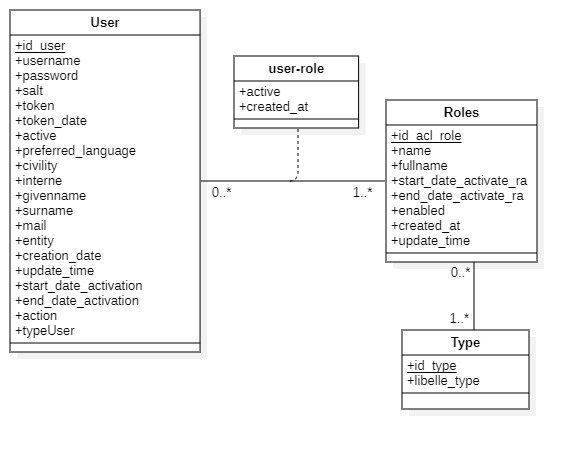
\includegraphics[width=0.7\linewidth]{img/conception/classes/ClassDiag-sprint1}
	\caption[Diagramme de classes de sprint 1]{Diagramme de classes de sprint 1}
	\label{fig:classdiag-sprint1}
\end{figure}
\subsection{Diagrammes de séquences détaillés}
Nous allons maintenant passer à l’aspect dynamique des opérations représentées dans le diagramme de classe à l’aide des diagrammes de séquences de système et d’objets.
\subsubsection{Quelques diagramme de séquences système de Sprint 1}
Dans cette section, nous présenterons quelques diagrammes de séquences système de \\sprint 1 tels que : \newpage
\myparagraph{Diagramme de séquences système d’«Ajouter Utilisateur»}\label{ajout-user}
Ce diagramme représenté dans la figure \ref{fig:add-user} explique graphiquement des interactions entre les acteurs et le système selon l'ordre chronologique. D'abord l'acteur accède à la page de création des utilisateurs et il remplit la formulaire. Le système vérifie les données saisies tel que les rôles, l'email,etc.\\Si l'ajout d'utilisateur se termine normalement un message de succès sera affiché sinon un message d'erreur sera affiché.
\begin{figure}[H]
	\centering
	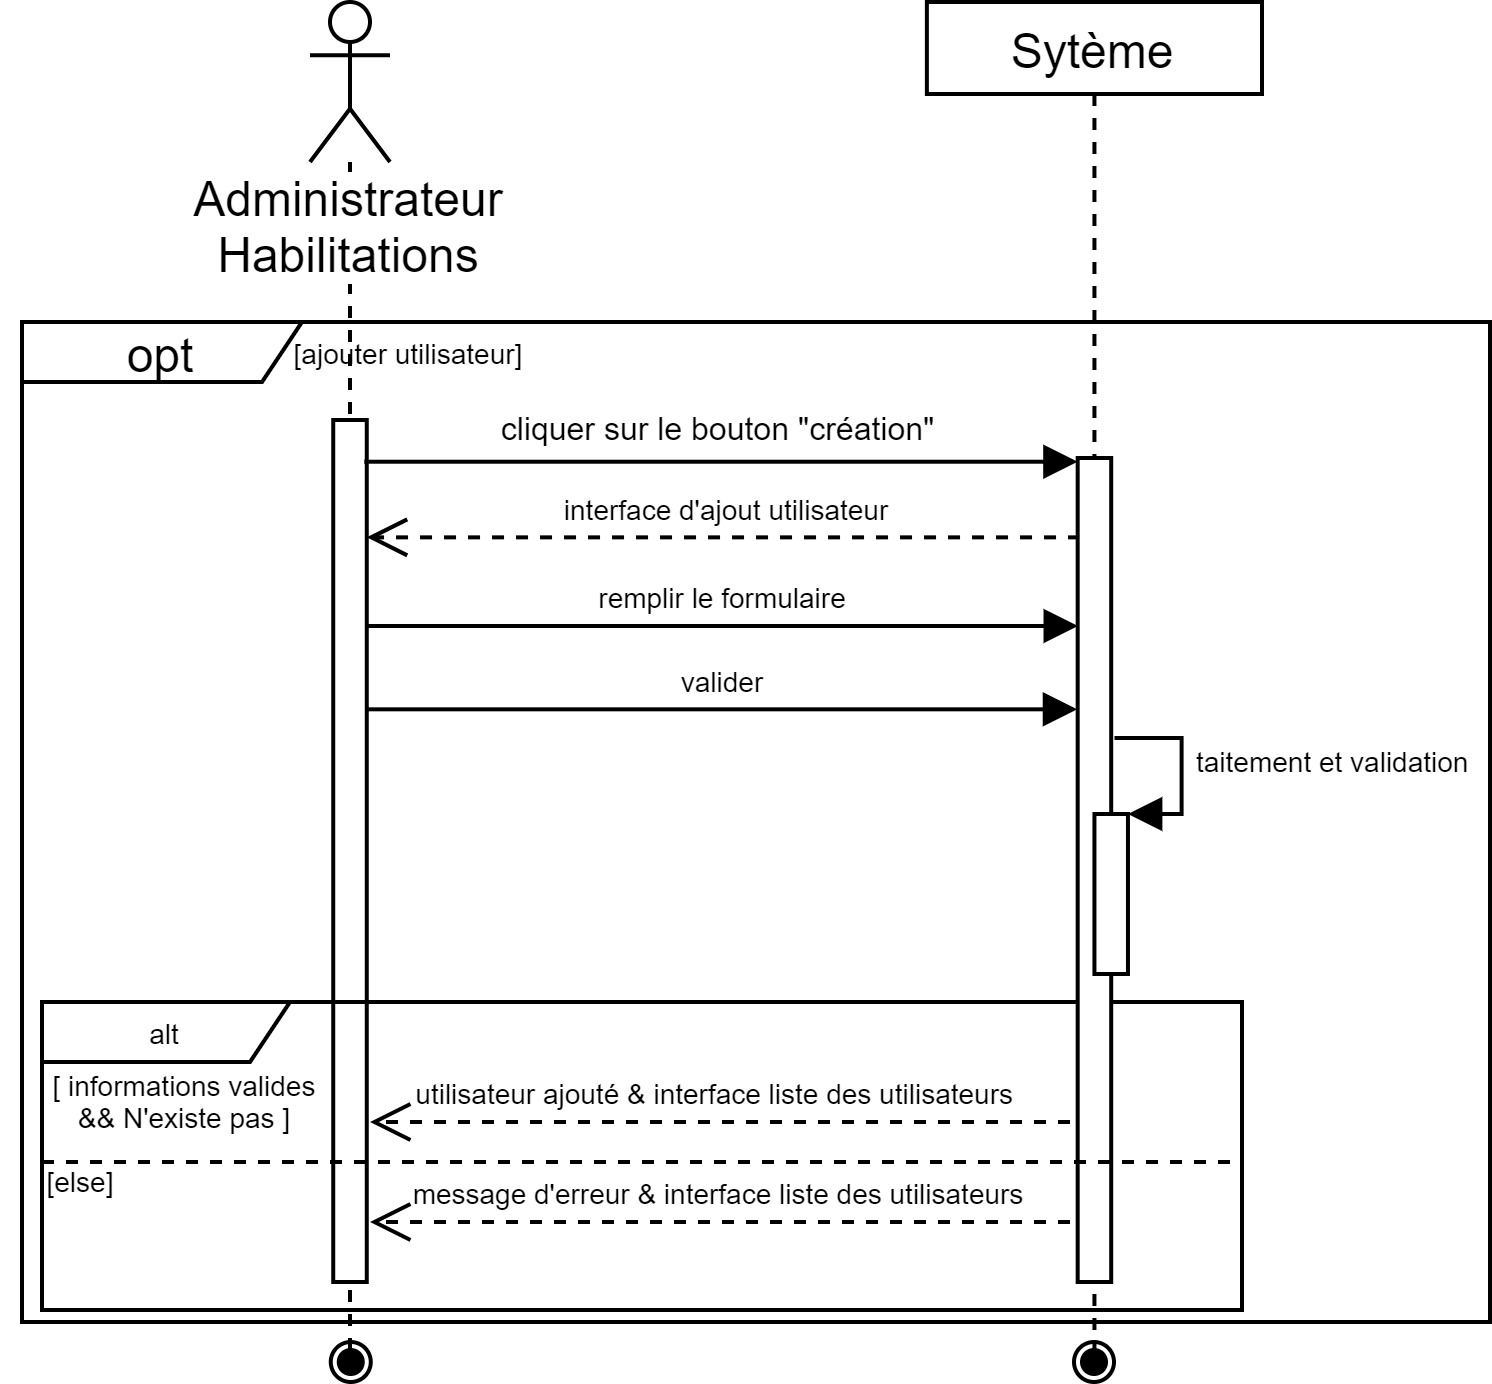
\includegraphics[width=0.65\linewidth]{img/conception/sequences/add-user}
	\caption[Diagramme de séquences système d’ «Ajouter Utilisateur»]{Diagramme de séquences système d’ «Ajouter Utilisateur»}
	\label{fig:add-user}
\end{figure}
\newpage
\myparagraph{Diagramme de séquences système de «Supprimer Utilisateur»}
La figure \ref{fig:delete-user} résume le scénario de suppression d'un utilisateur. Tout d'abord, l'administrateur choisi l'utilisateur à supprimer puis il clique sur le bouton de suppression. Le système vérifie l'existence de cet utilisateur. Un message de succès ou d'échec sera affiché.
\begin{figure}[H]
	\centering
	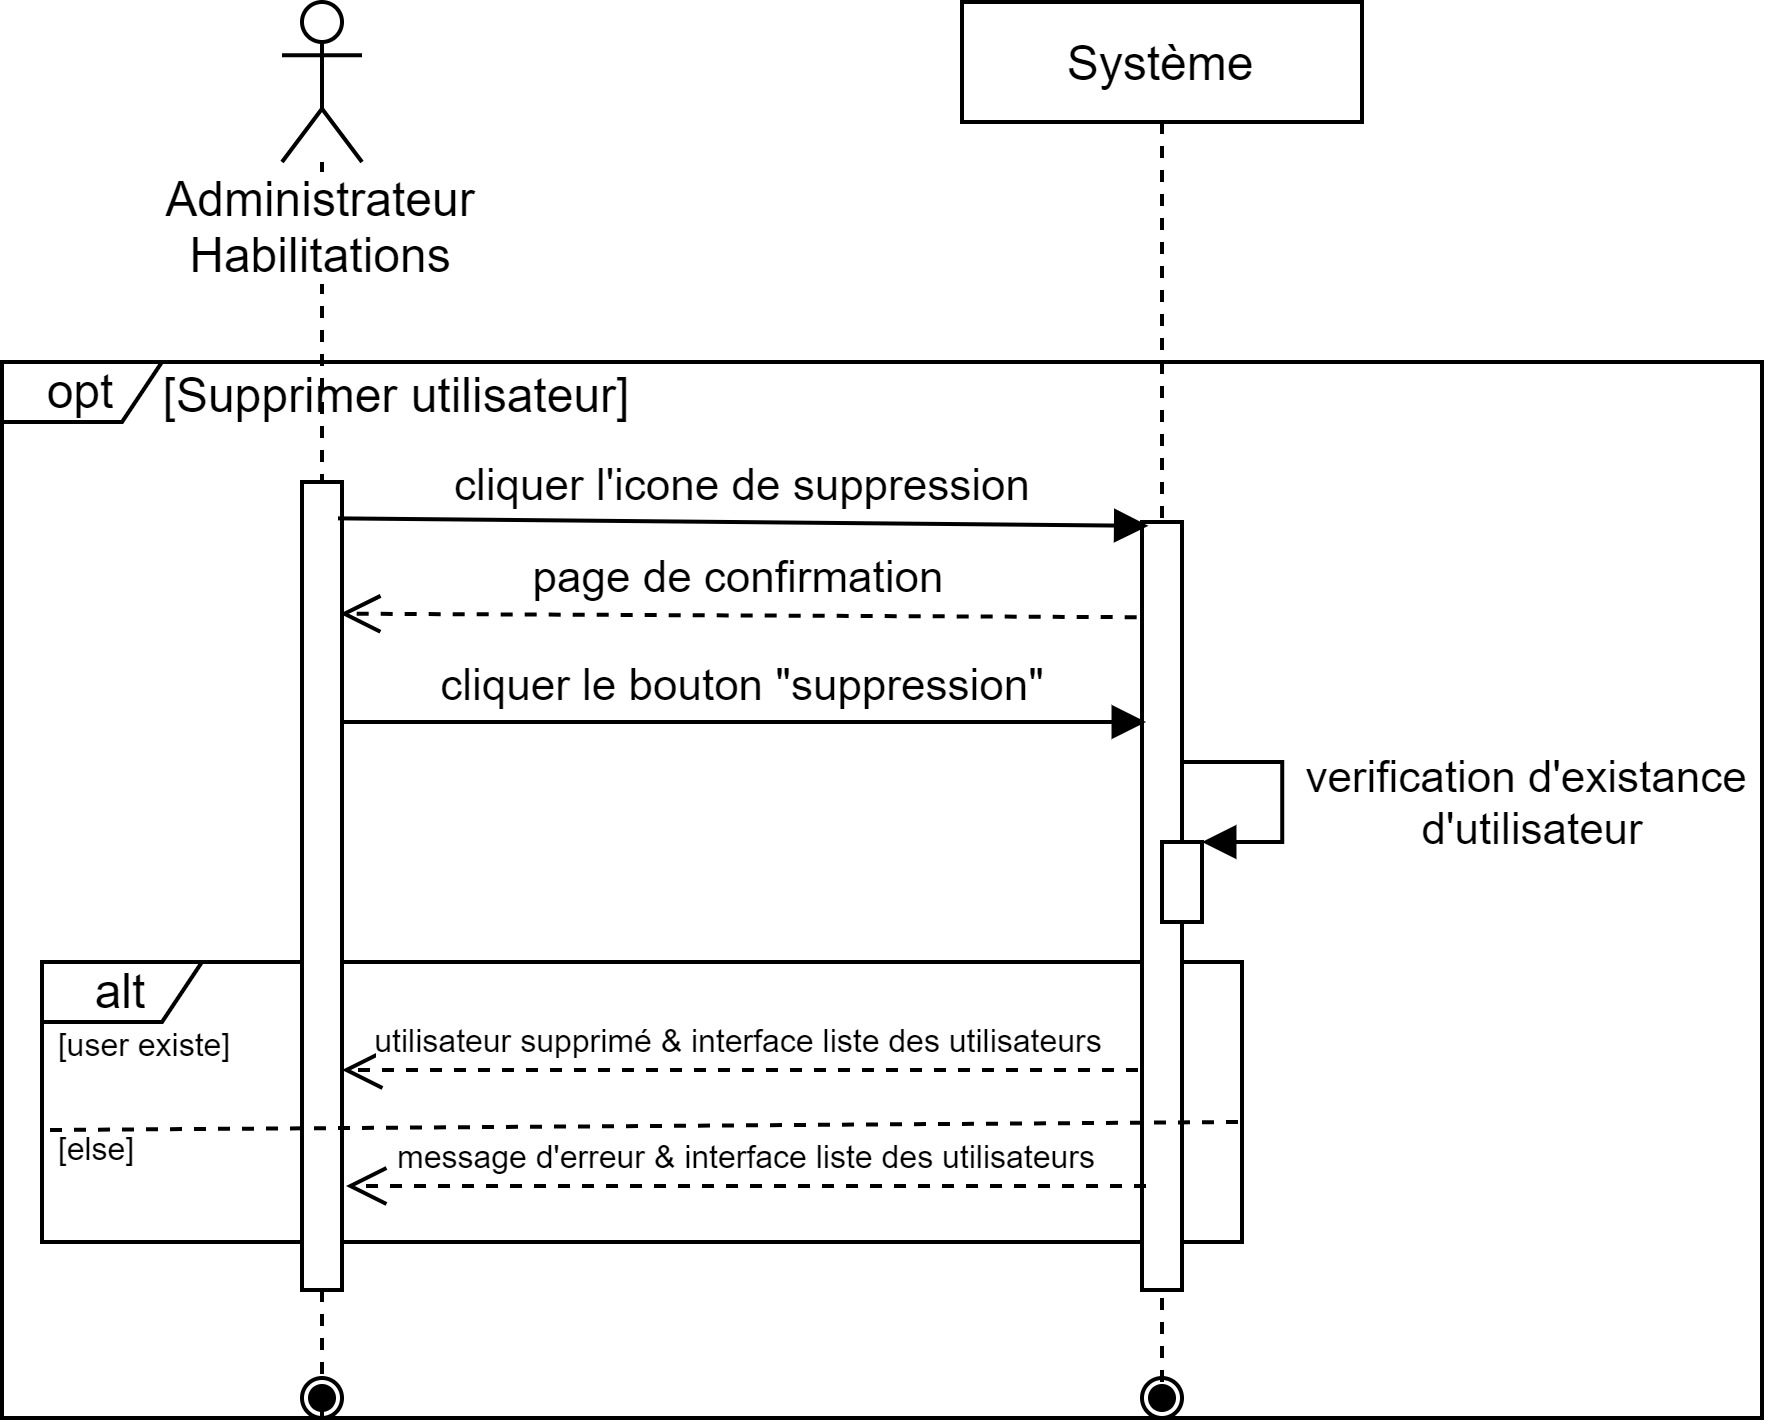
\includegraphics[width=0.65\linewidth]{img/conception/sequences/delete-user}
	\caption[Diagramme de séquences système de «Supprimer Utilisateur»]{Diagramme de séquences système de «Supprimer Utilisateur»}
	\label{fig:delete-user}
\end{figure}
\newpage
\myparagraph{Diagramme de séquences système d’«Importer utilisateurs»}
La figure \ref{fig:import} représente le scénario d'import des utilisateurs. Après l'upload de fichier CSV, le système vérifie la structure du fichier. Si ce dernier est bien structuré, et pour chaque ligne de fichier, le système vérifie la colonne action. Si la colonne action contient le mot "ADD" donc il va ajouter cet utilisateur dont ces informations sont dans cette ligne, sinon il va le supprimer.\\
Un message sera affiché pour indiquer l'état de terminaison de processus.  
\begin{figure}[H]
	\centering
	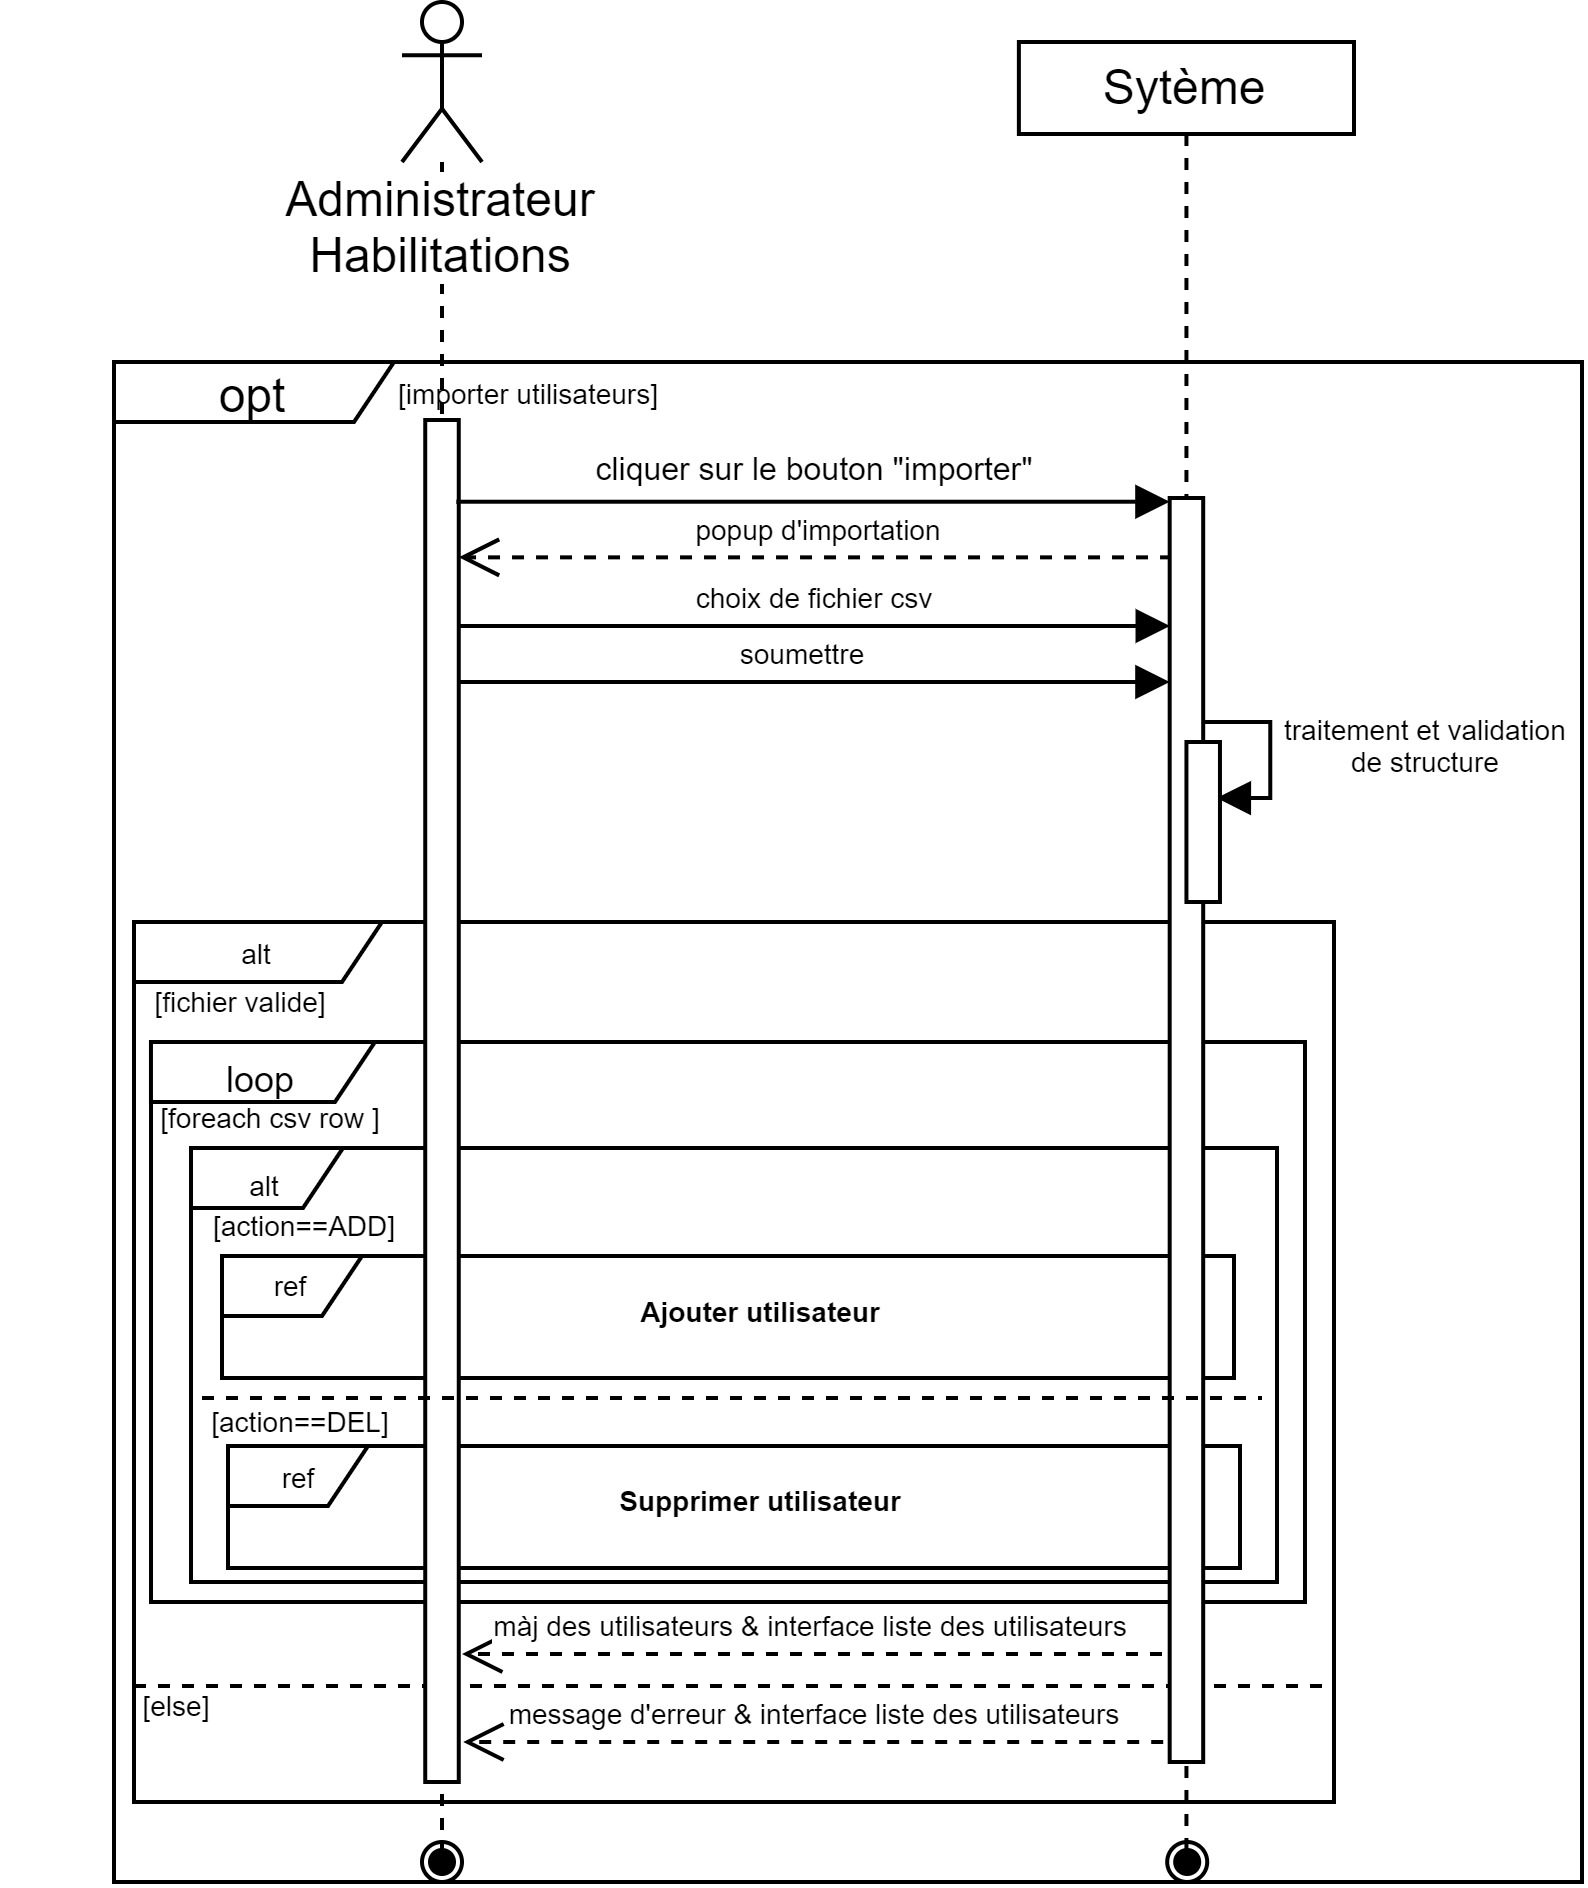
\includegraphics[width=0.65\linewidth]{img/conception/sequences/import}
	\caption[Diagramme de séquences système d’ «Importer utilisateurs»]{Diagramme de séquences système d' «Importer utilisateurs»}
	\label{fig:import}
\end{figure}

\subsubsection{Diagramme de séquences objets de Sprint 1}
Nous présentons dans ce qui suit quelques diagrammes de séquences objets détaillés du \\sprint 1.
\newpage
\myparagraph{Diagramme de séquences objets d’«Ajouter Utilisateur» } 
Nous ajoutons à la description de la figure \ref{fig:add-user} l'appel de web service qui permet de changer la liste des rôles selon le type de l'utilisateur choisi.
\begin{figure}[H]
	\centering
	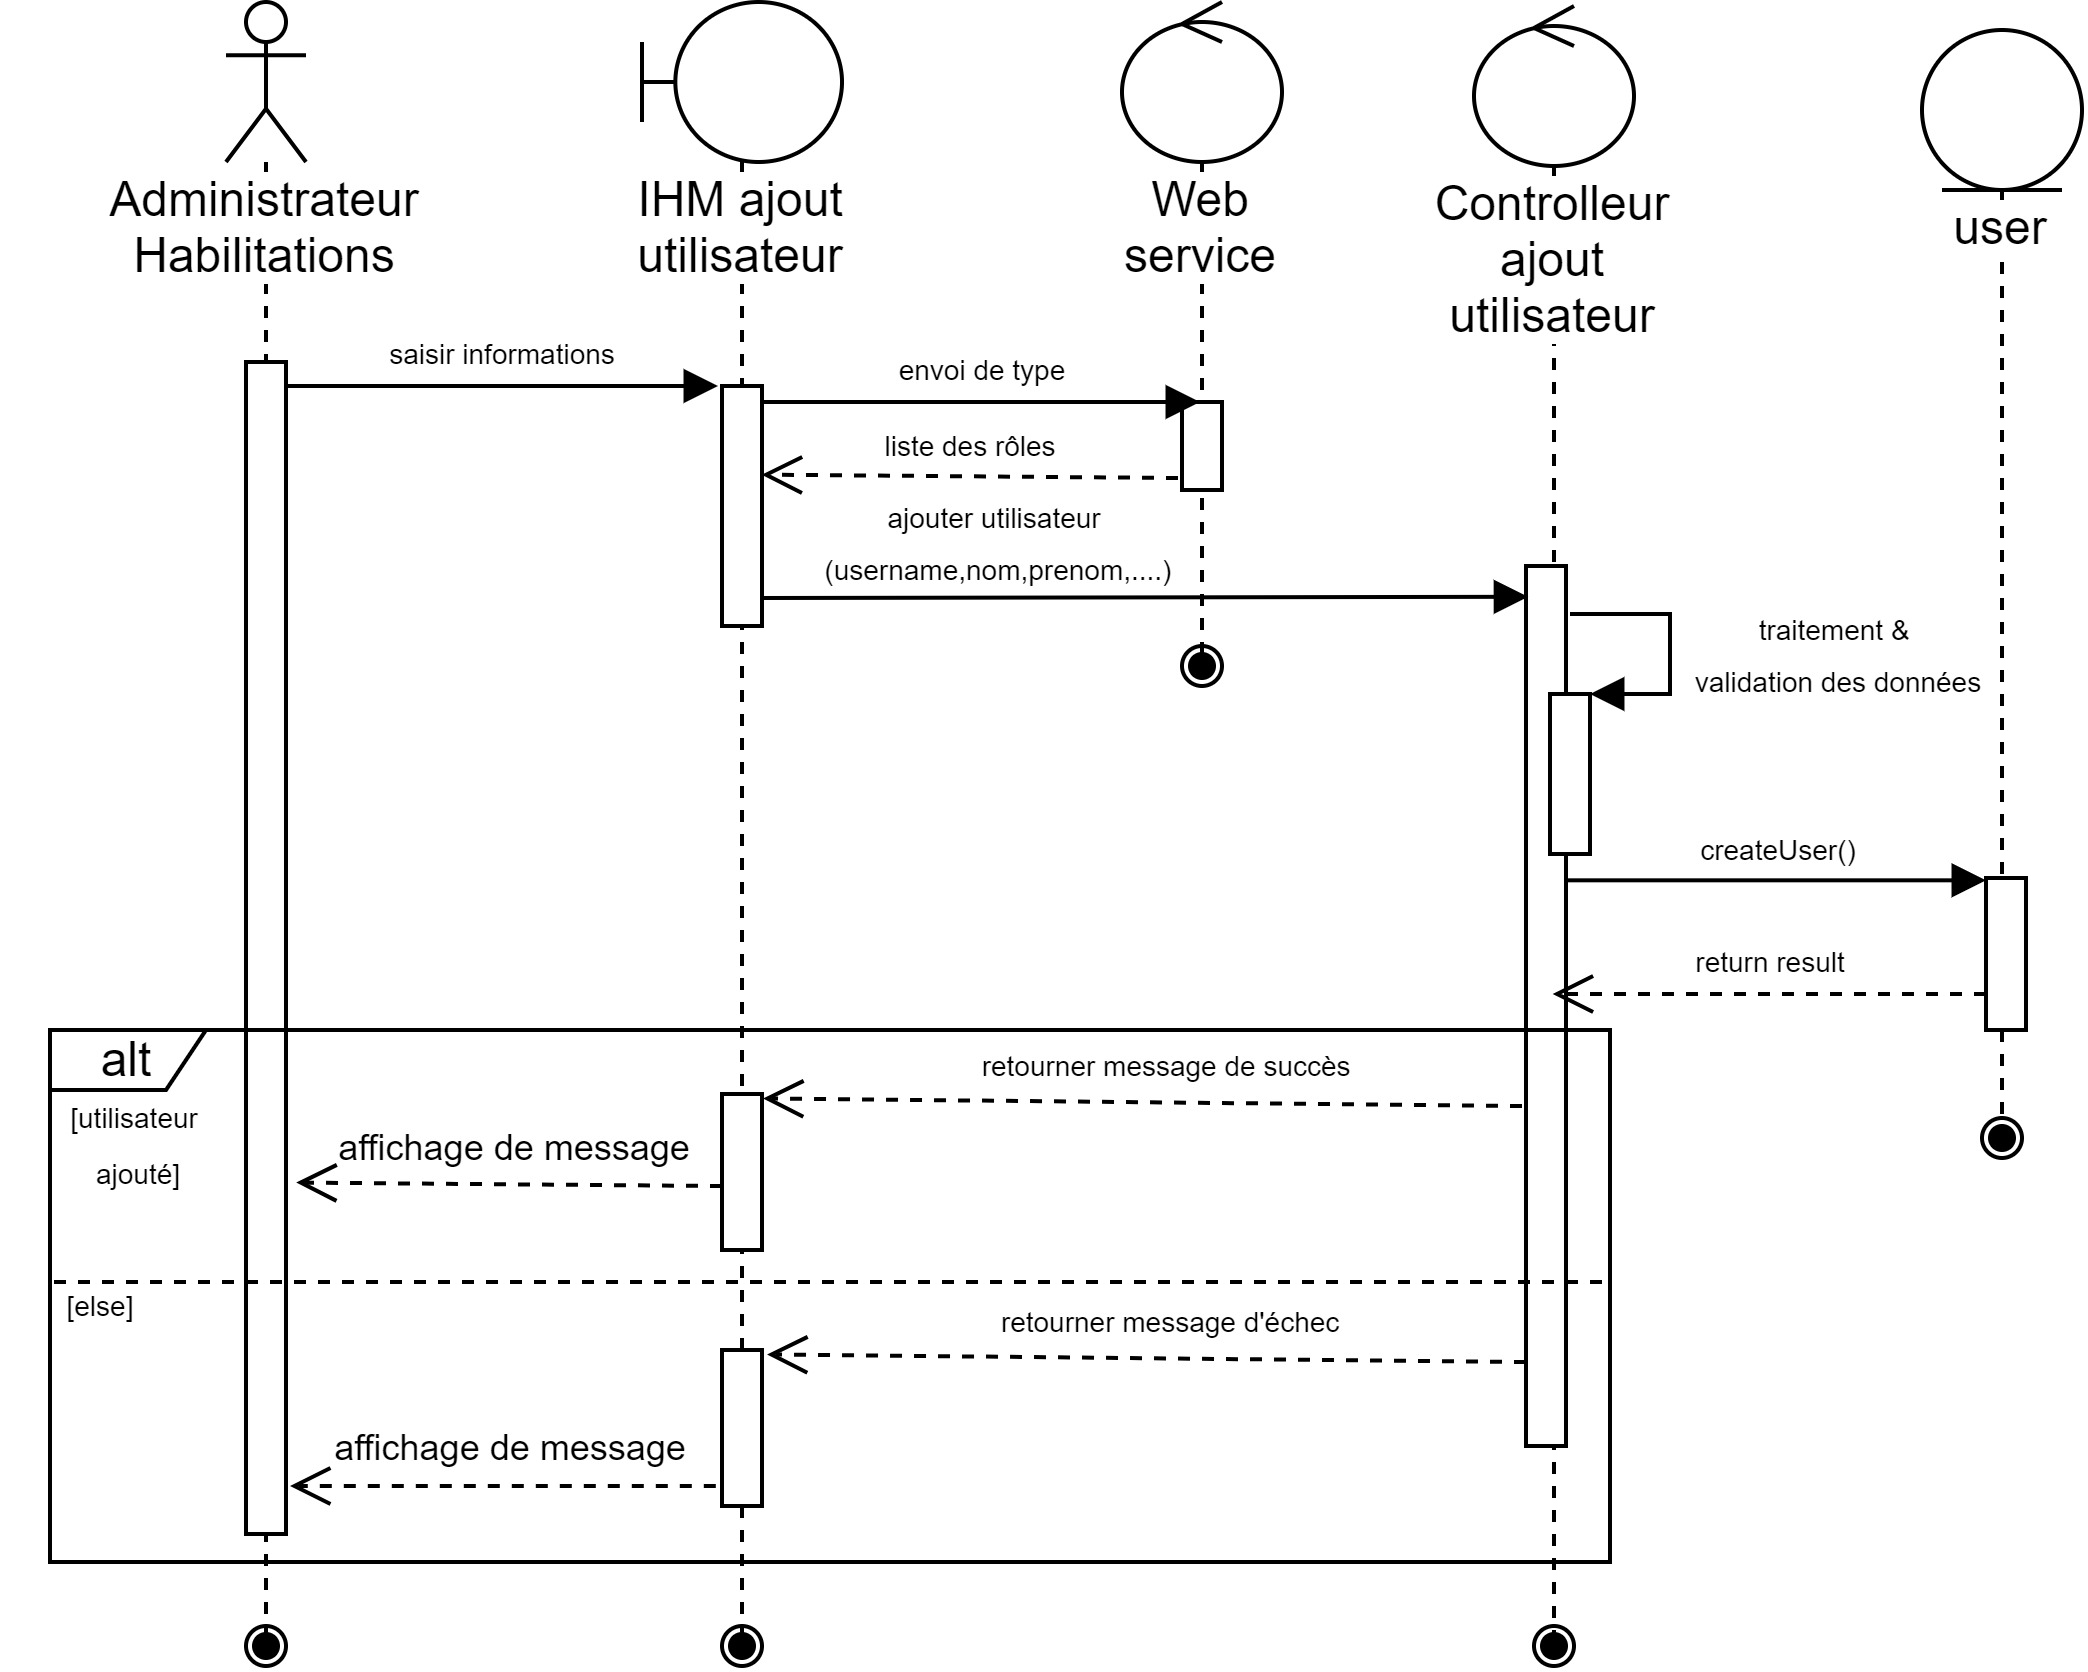
\includegraphics[width=0.75\linewidth]{img/conception/sequences/add-user-obj}
	\caption[Diagramme de séquences objets d’«Ajouter Utilisateur»]{Diagramme de séquences objets d’«Ajouter Utilisateur»}
	\label{fig:add-user-obj}
\end{figure}

\myparagraph{Diagramme de séquences objets de «Supprimer Utilisateur» }
\begin{figure}[H]
	\centering
	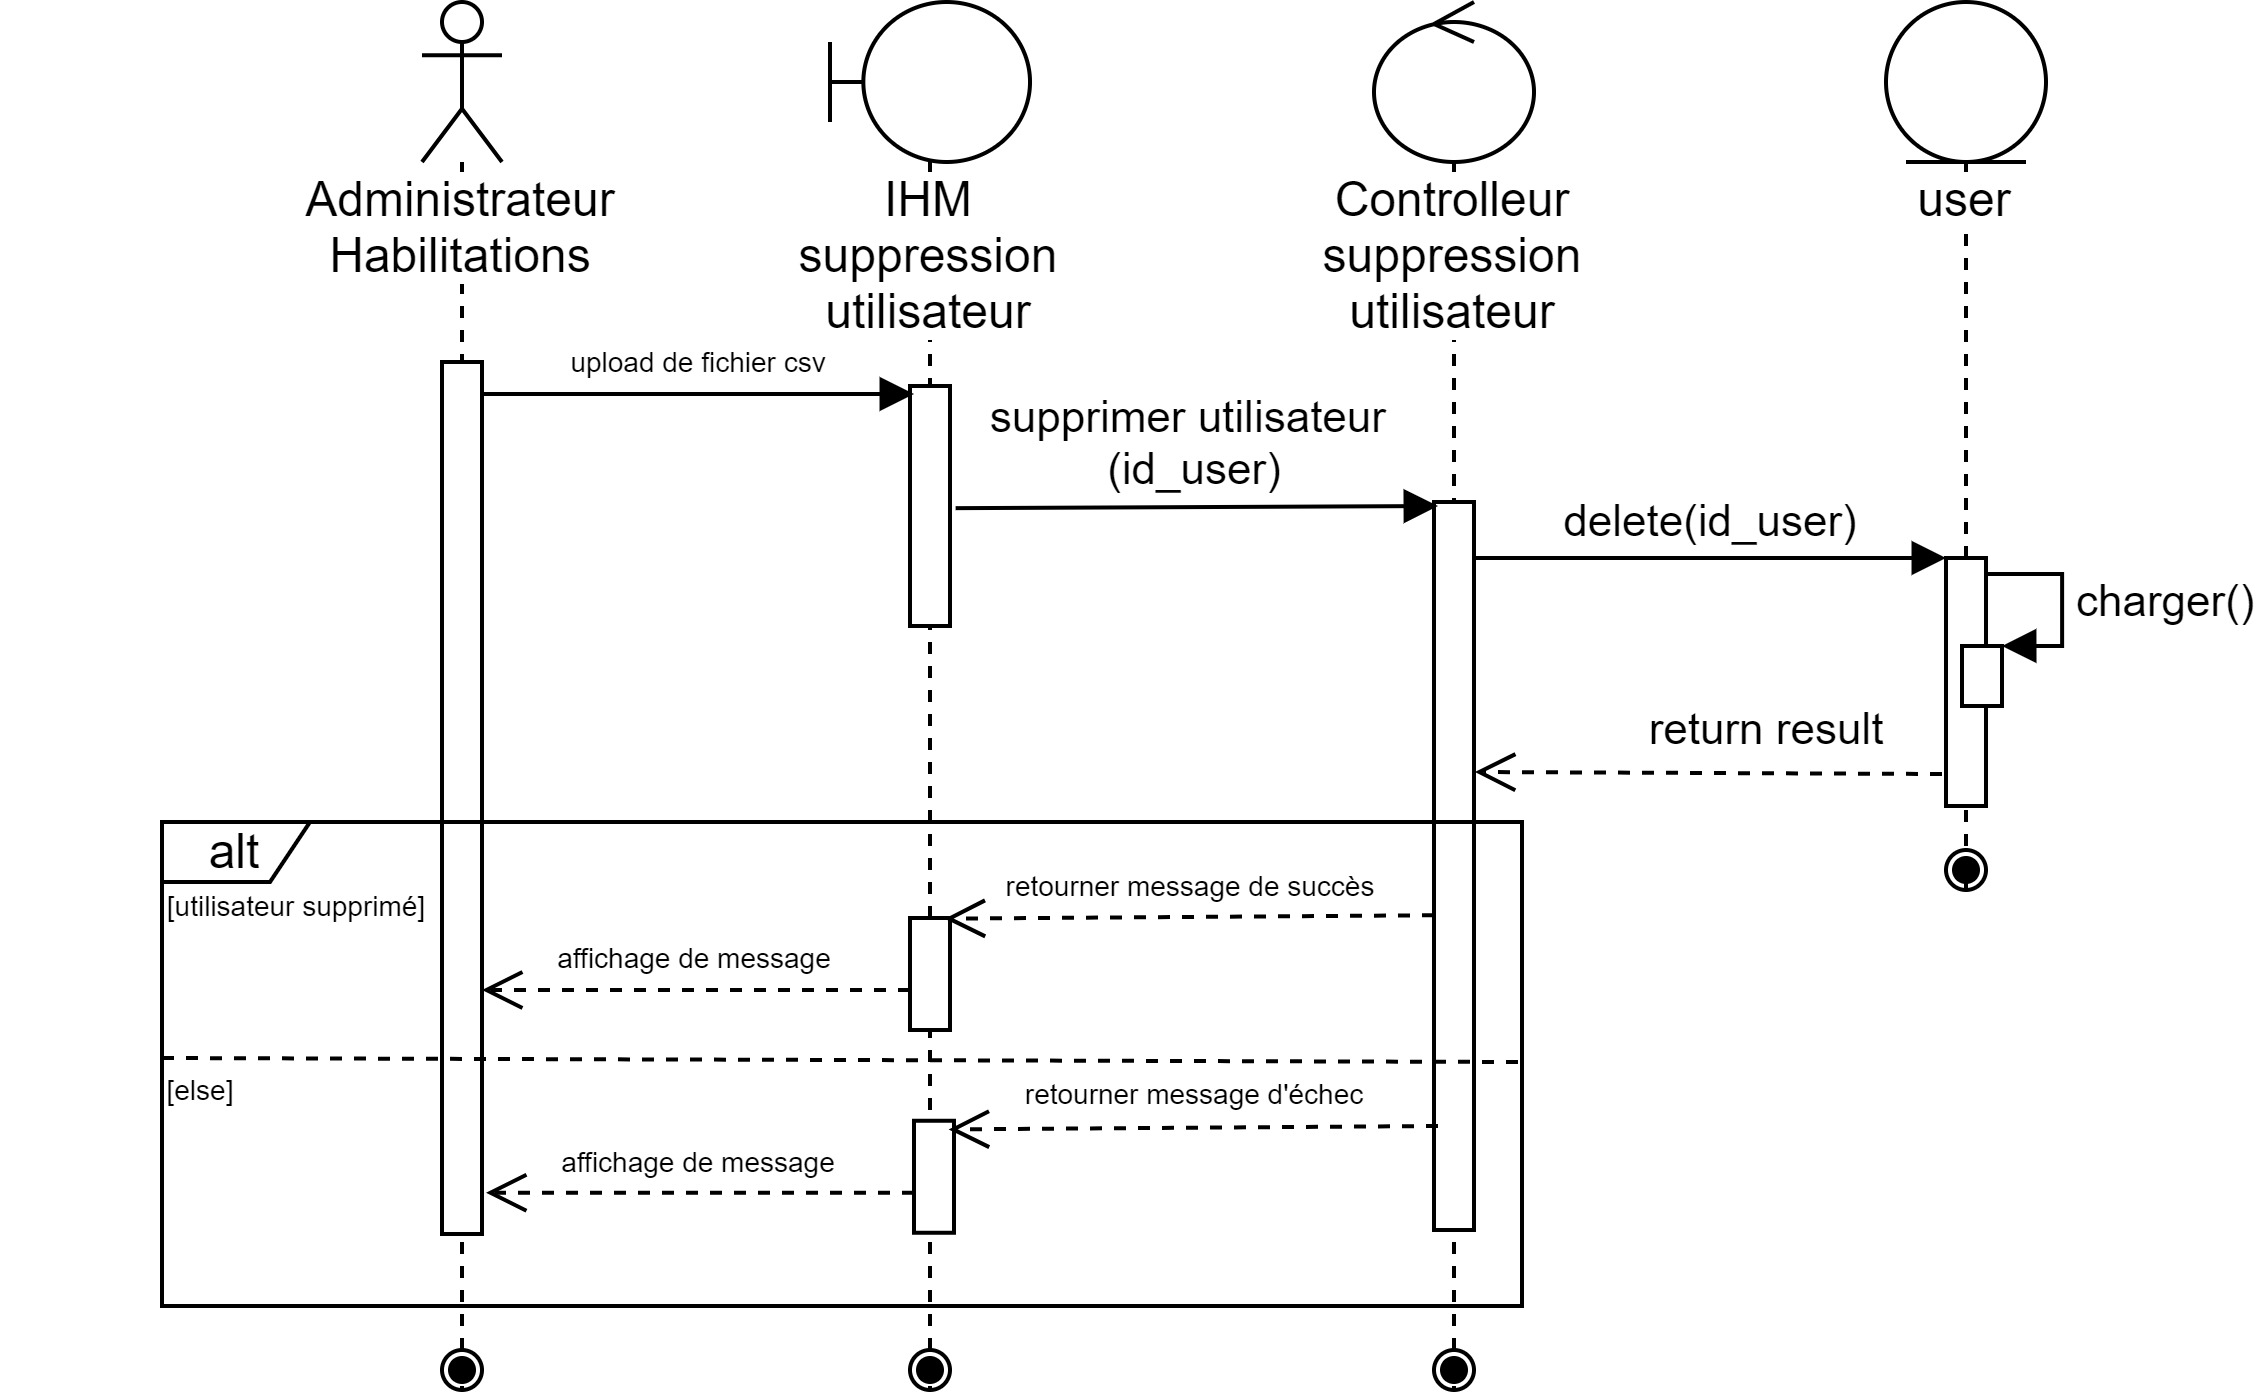
\includegraphics[width=0.75\linewidth]{img/conception/sequences/delete-obj}
	\caption[Diagramme de séquences objets de «Supprimer Utilisateur»]{Diagramme de séquences objets de «Supprimer Utilisateur»}
	\label{fig:delete-obj}
\end{figure}

\section[Réalisation]{Réalisation}
Dans cette sous-sections nous allons exposer les différentes interfaces réalisées dans le \\sprint 1. 
\subsection[Interfaces de gestion des utilisateurs]{Interfaces de gestion des utilisateurs}
les captures d'écran ci-dessous représentent les différentes IHM de gestion des utilisateurs.
\begin{itemize}
	\item Consultation des utilisateurs \& recherche
	\begin{figure}[H]
		\centering
		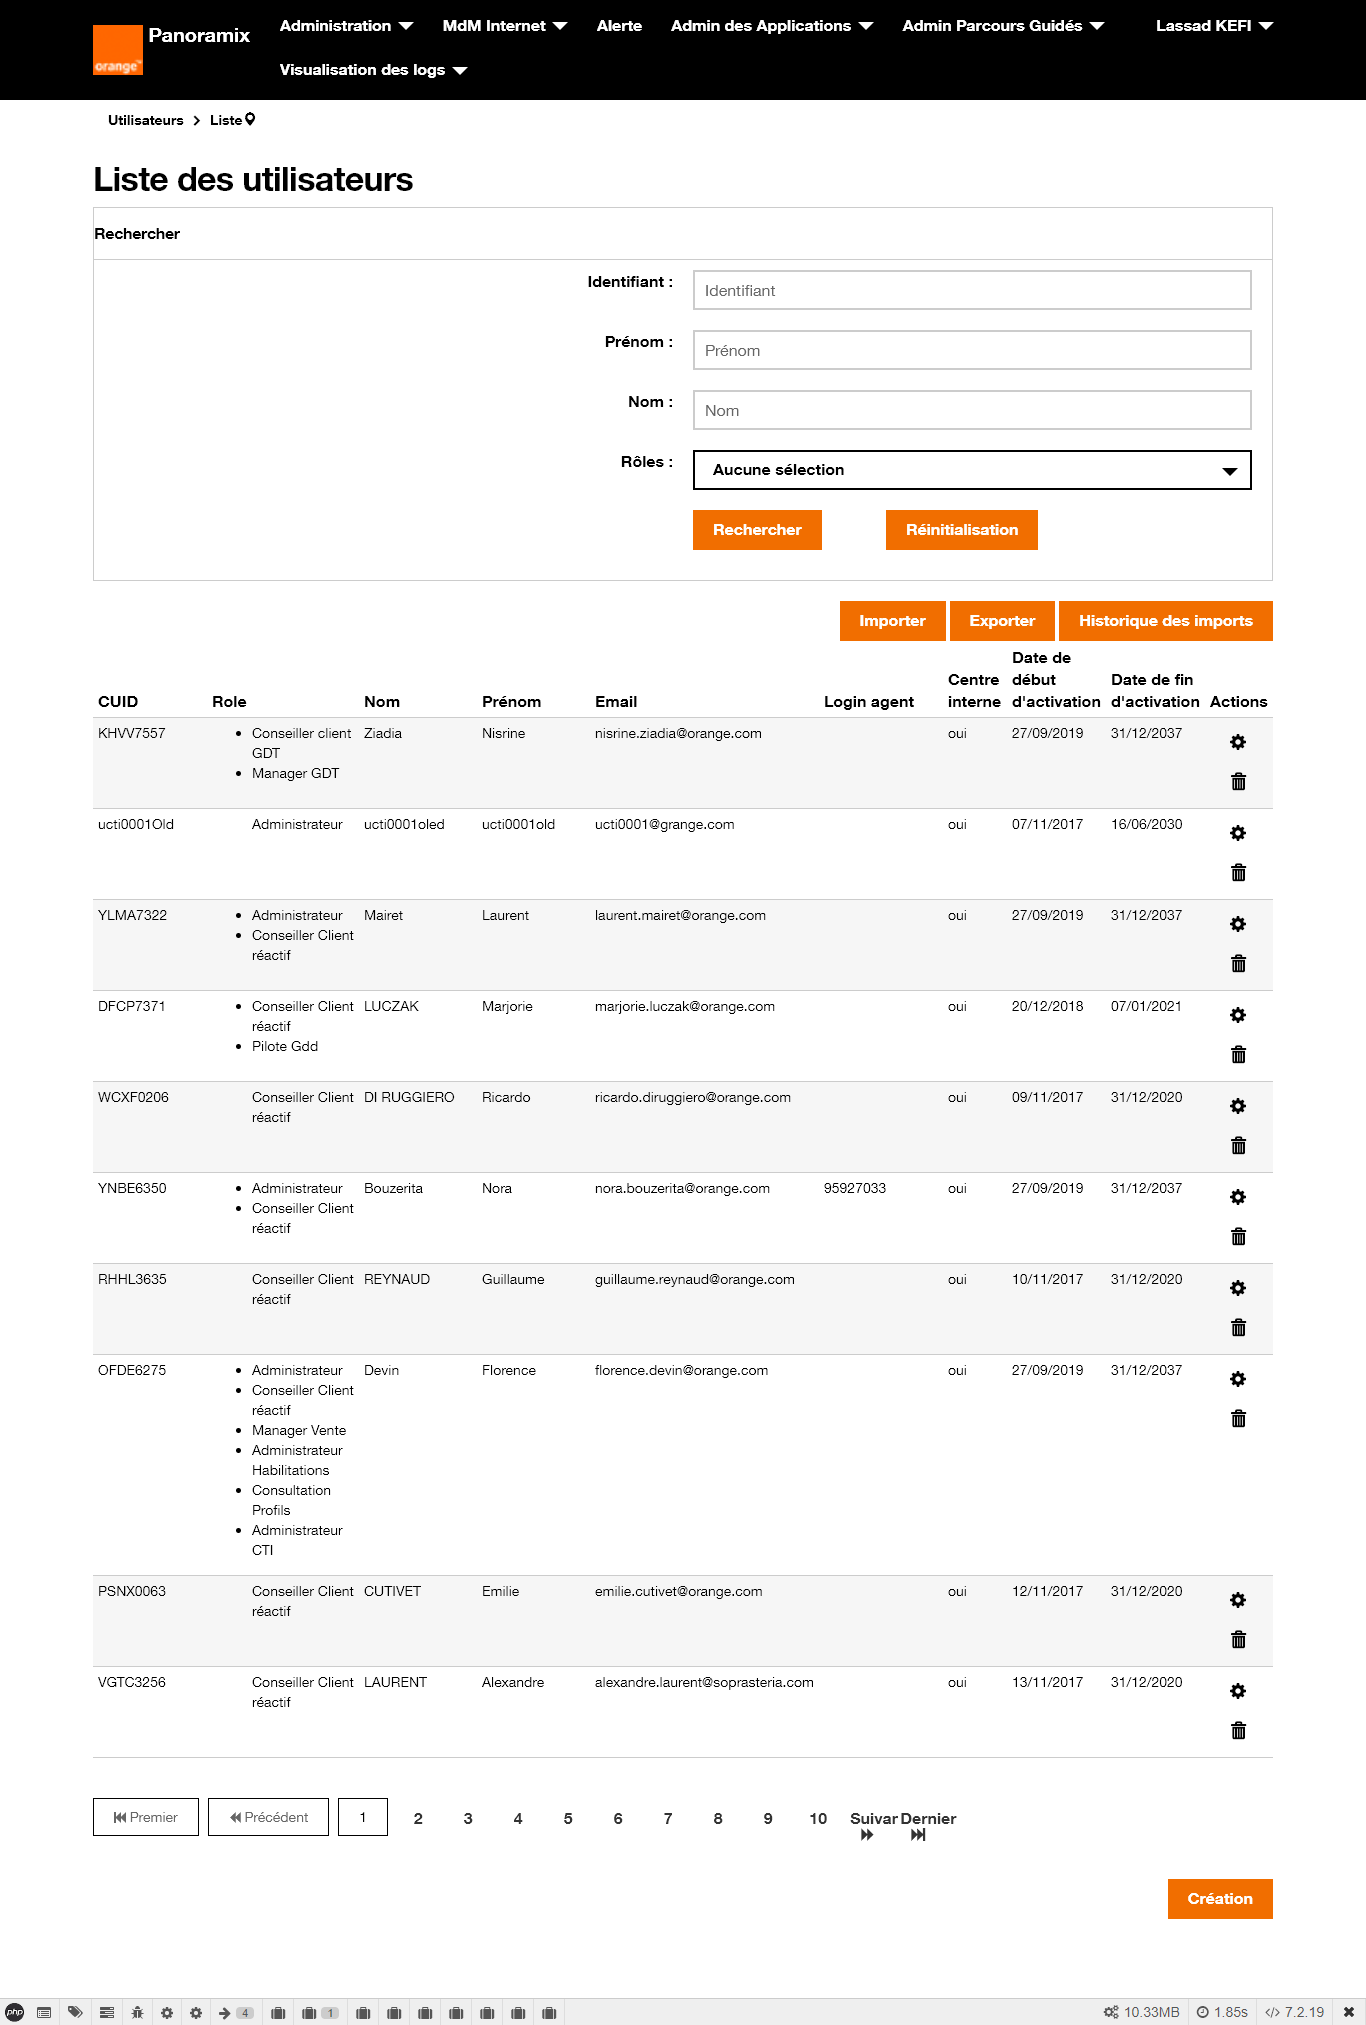
\includegraphics[width=0.7\linewidth]{img/screenshots/users/consultation}
		\caption[Interface consultation des utilisateurs et recherche]{Interface consultation des utilisateurs et recherche}
		\label{fig:consultation-user}
	\end{figure}
	\newpage
	\item Consulter les données d'un utilisateur
	\begin{figure}[H]
		\centering
		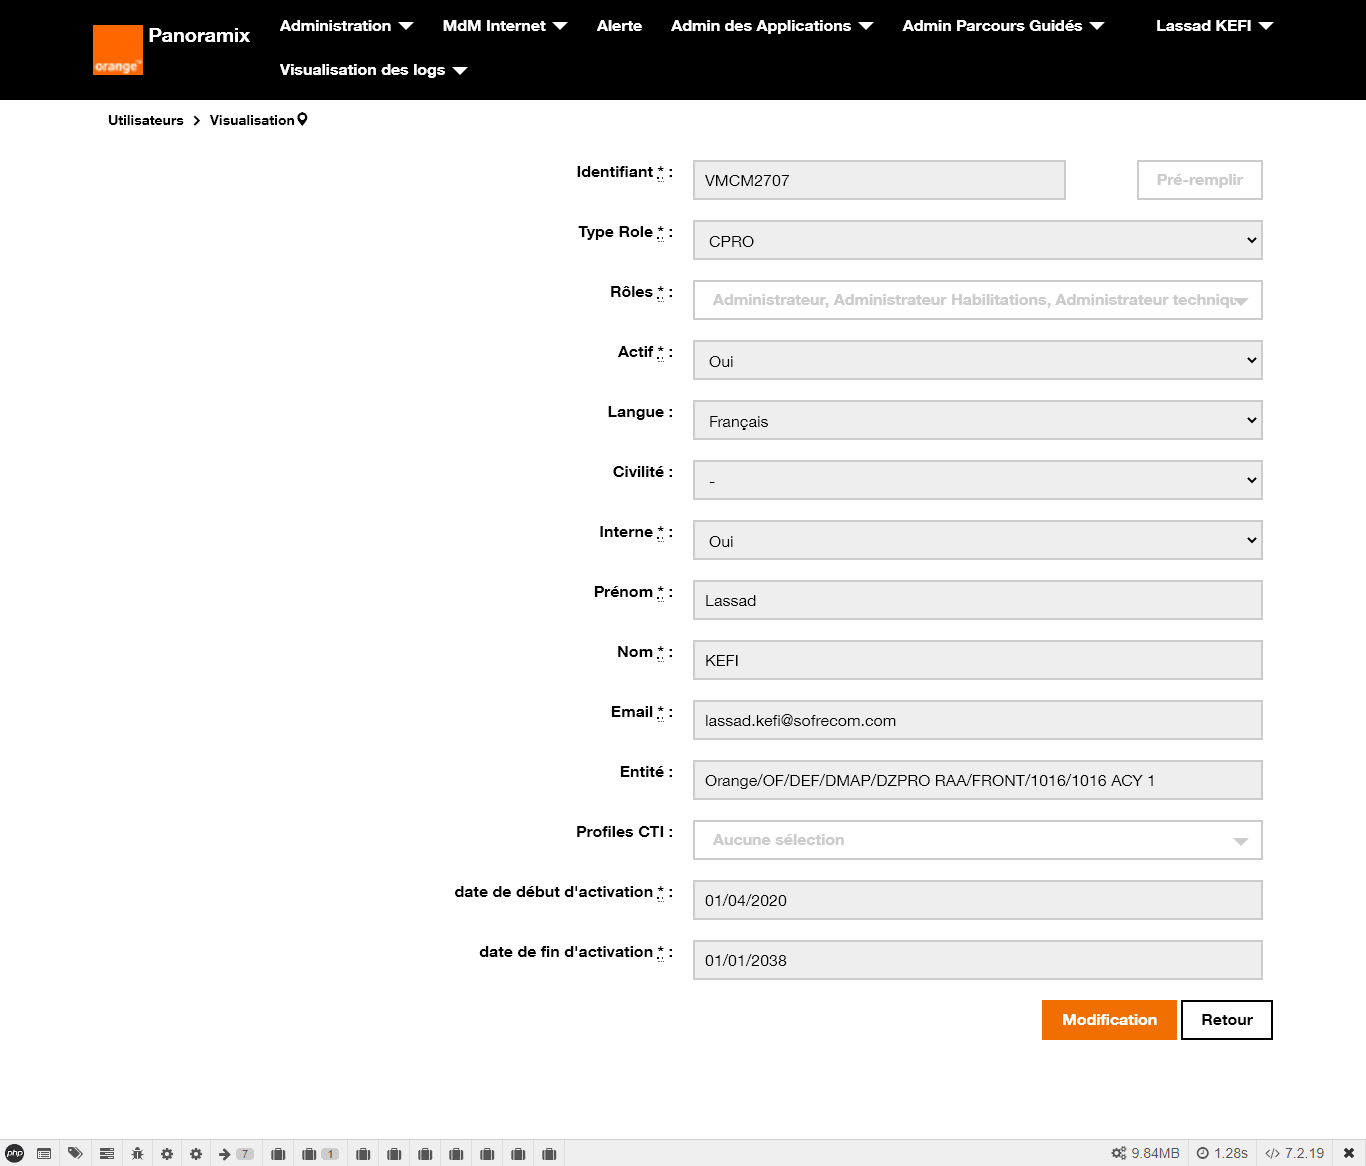
\includegraphics[width=0.65\linewidth]{img/screenshots/users/view}
		\caption[Interface voir utilisateur]{Interface consulter les données d'un utilisateur}
		\label{fig:view-user}
	\end{figure}

	\item Modifier ou créer utilisateur
	\begin{figure}[H]
		\centering
		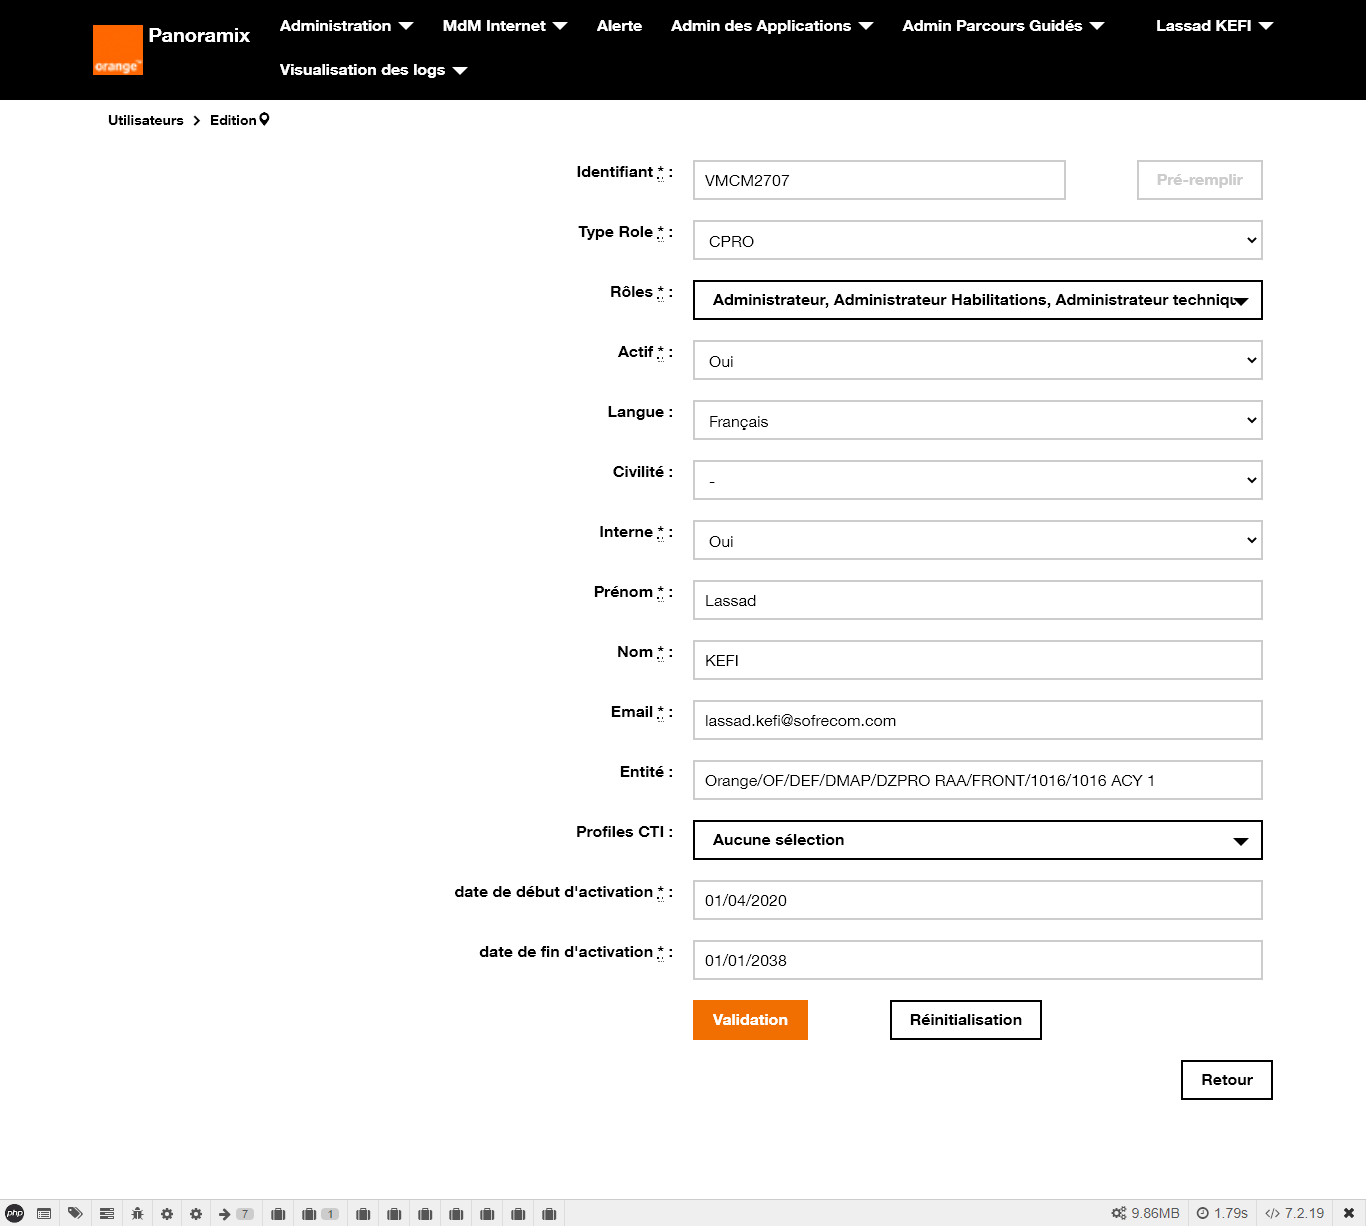
\includegraphics[width=0.65\linewidth]{img/screenshots/users/modif}
		\caption[Interface modifier ou créer utilisateur]{Interface modifier ou créer utilisateur}
		\label{fig:modif-user}
	\end{figure}
	\newpage
	\item Supprimer utilisateur
	\begin{figure}[H]
		\centering
		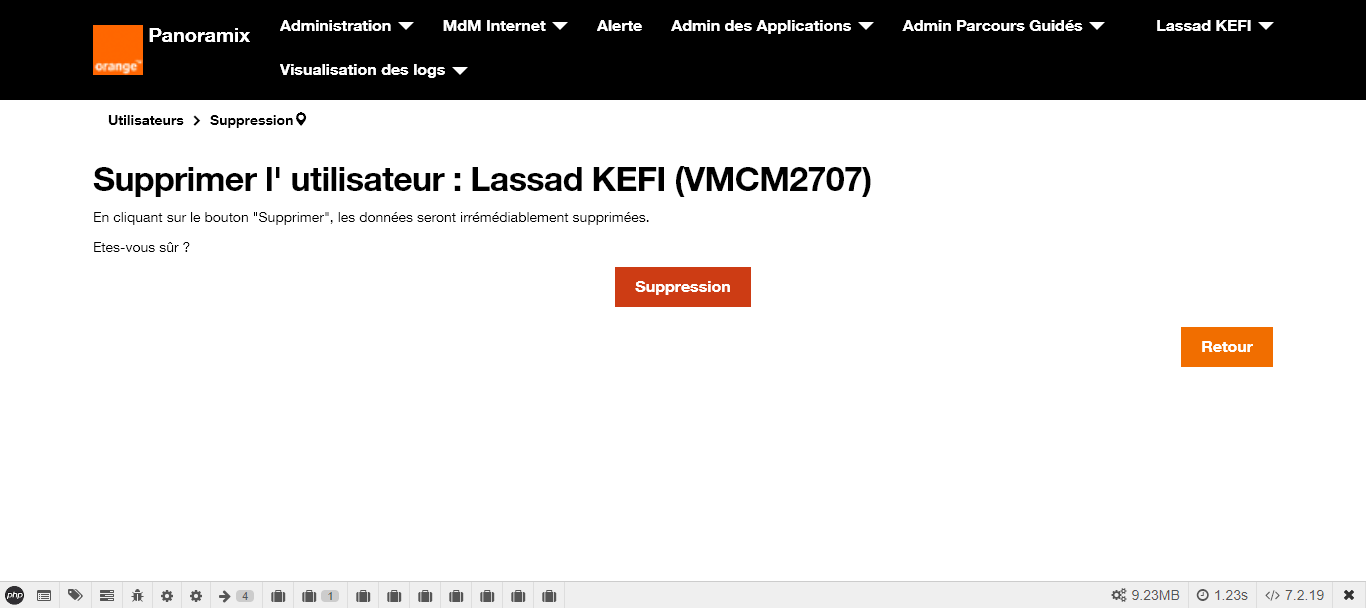
\includegraphics[width=0.65\linewidth]{img/screenshots/users/delete}
		\caption[Interface supprimer utilisateur]{Interface supprimer utilisateur}
		\label{fig:delete-user-ihm}
	\end{figure}

	\item Importer utilisateurs
	\begin{figure}[H]
		\centering
		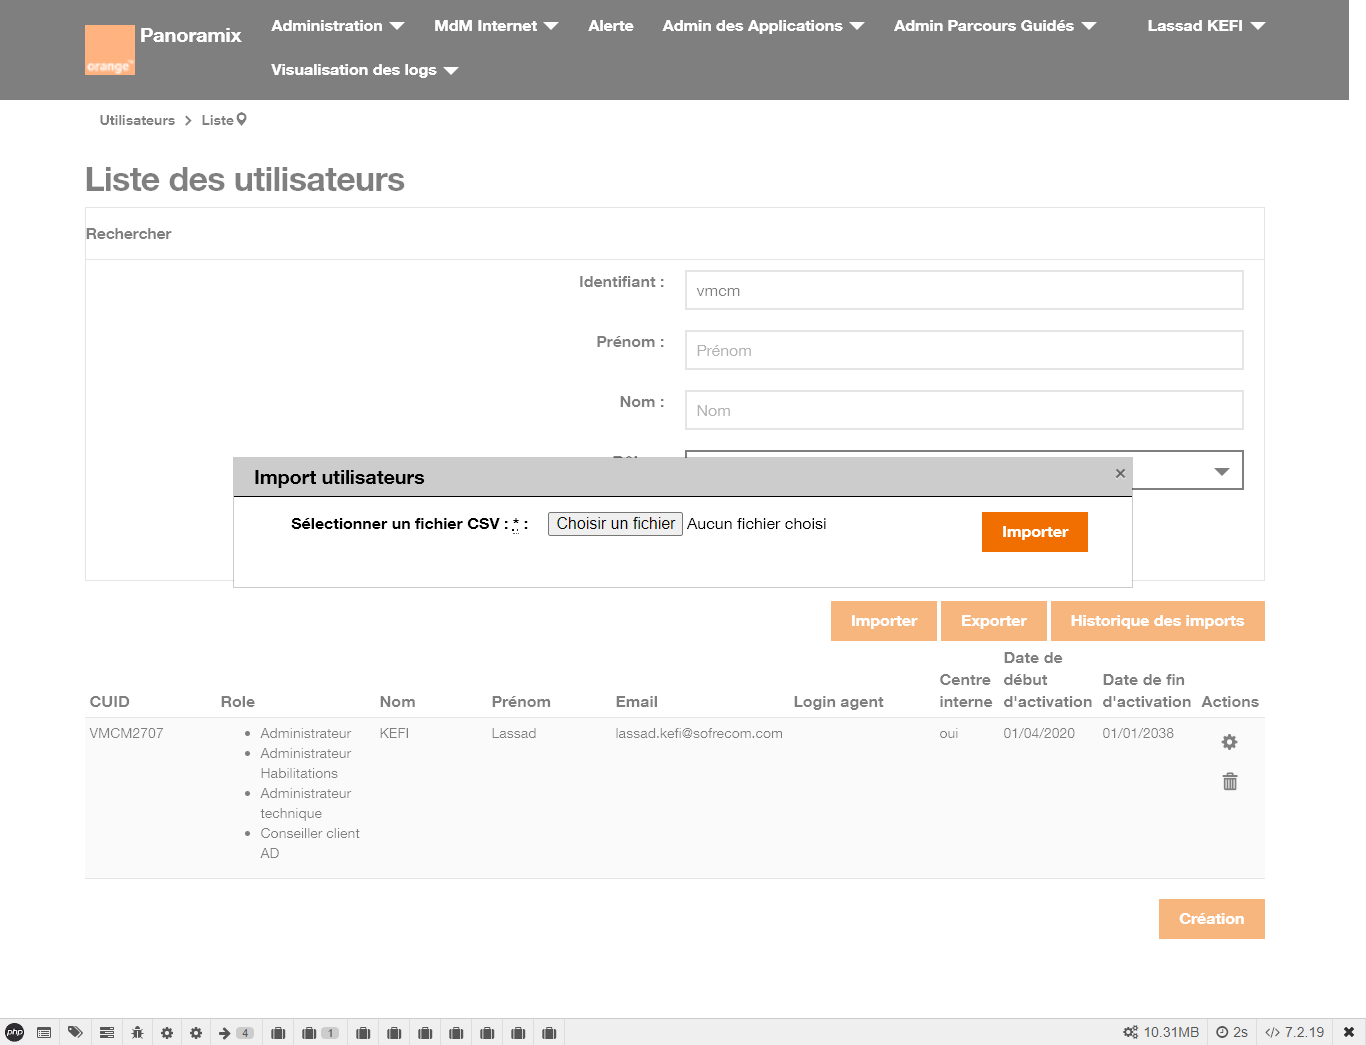
\includegraphics[width=0.65\linewidth]{img/screenshots/users/import}
		\caption[Interface importer utilisateurs]{Interface importer utilisateurs}
		\label{fig:import-user-ihm}
	\end{figure}

	\item Résultat d'exportation des utilisateurs
	\begin{figure}[H]
		\centering
		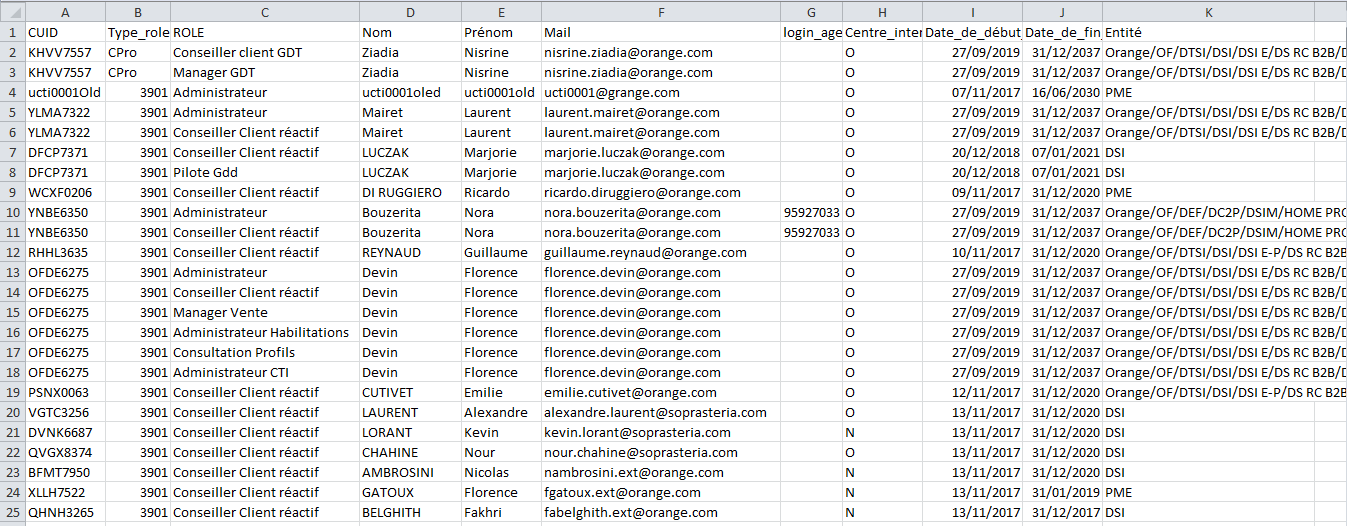
\includegraphics[width=0.65\linewidth]{img/screenshots/users/export}
		\caption[Extrait de résultat d'exportation des utilisateurs]{Interface résultat d'exportation des utilisateurs}
		\label{fig:export-user-ihm}
	\end{figure}
\end{itemize}

\subsection{Interfaces de gestion des rôles}
les captures d'écran ci-dessous représentent les différentes IHM de gestion des rôles.
\begin{itemize}
	\item Consultation des rôles et recherche
	\begin{figure}[H]
		\centering
		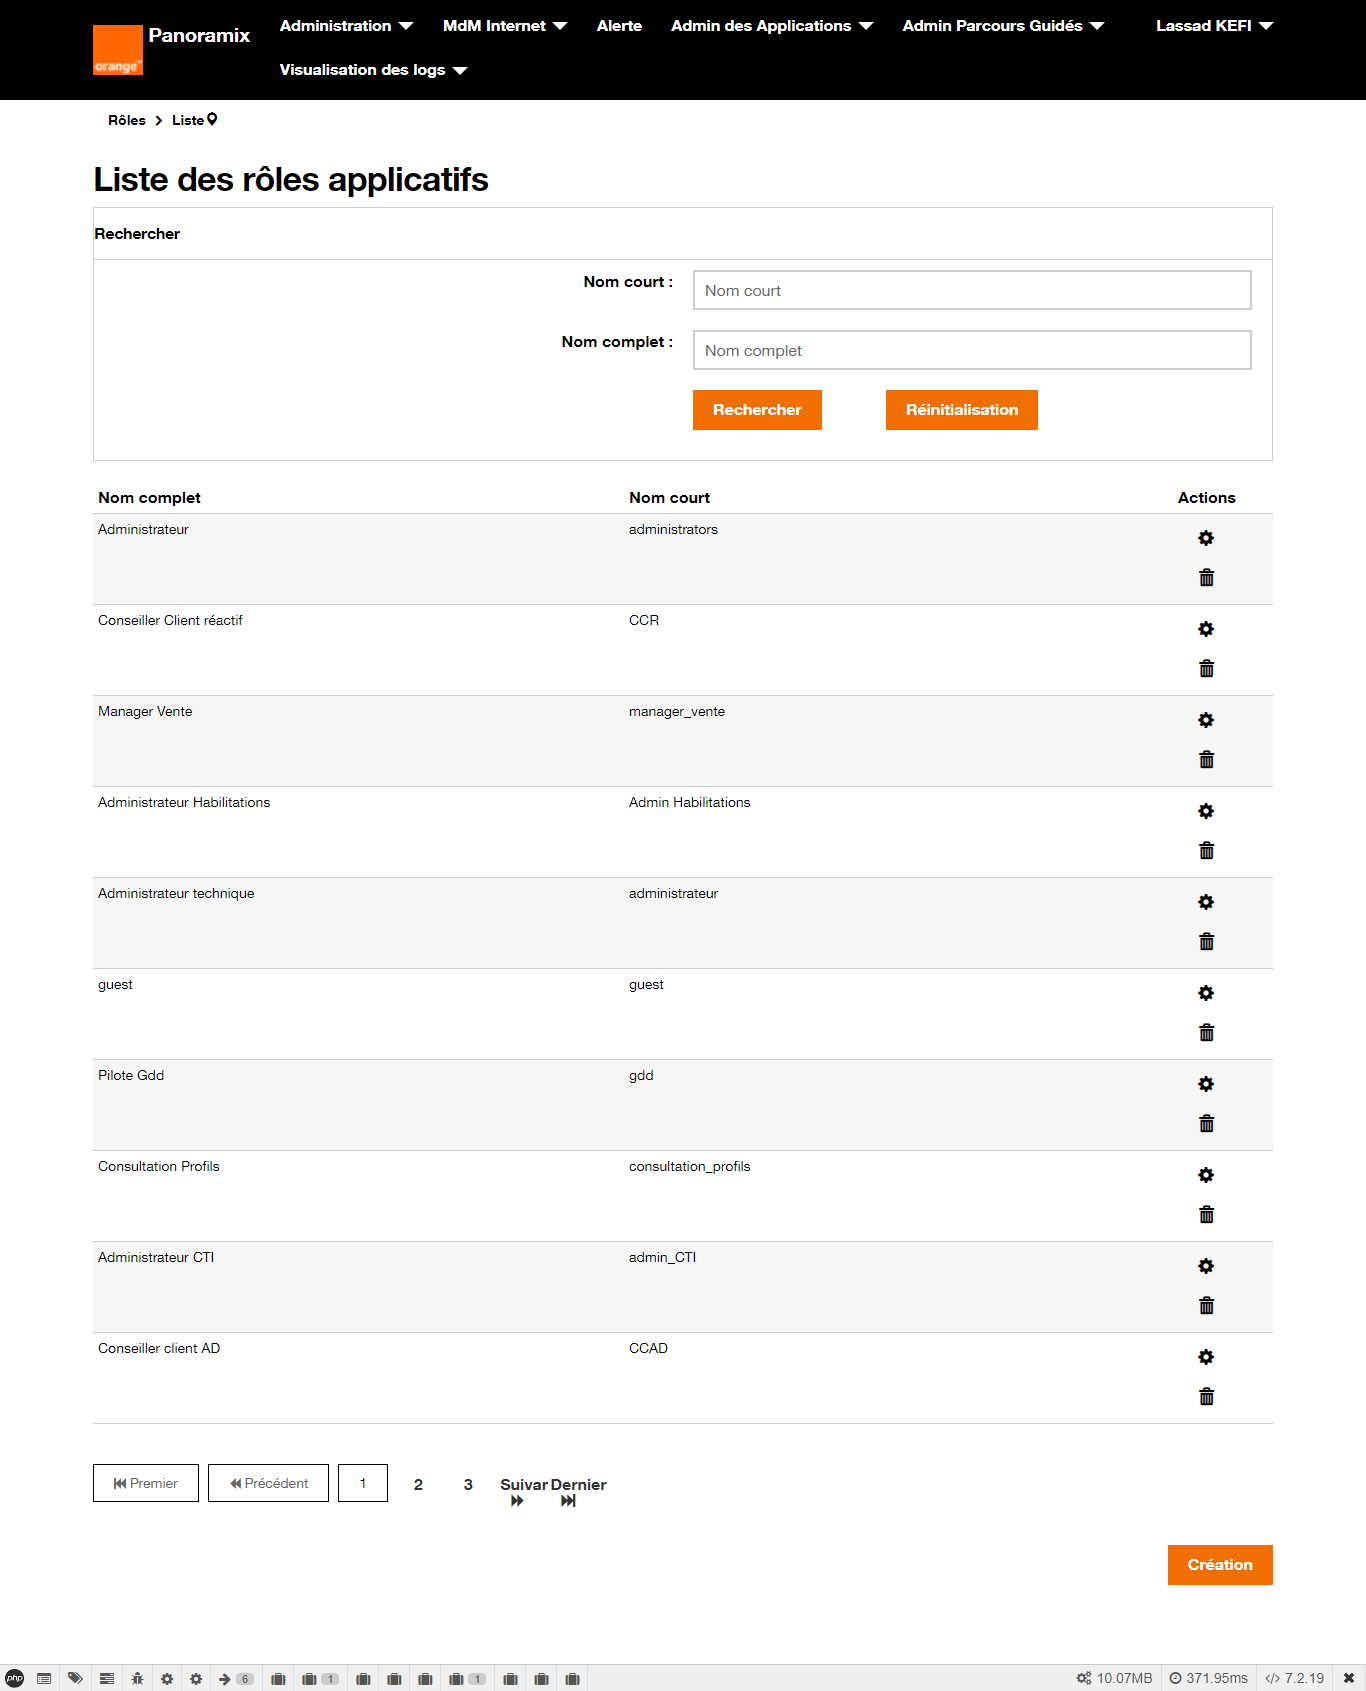
\includegraphics[width=0.65\linewidth]{img/screenshots/roles/index}
		\caption[Interface consultation des rôles]{Interface consultation des rôles et recherche}
		\label{fig:index-roles}
	\end{figure}
	
	\item Consulter les données d'un rôle
	\begin{figure}[H]
		\centering
		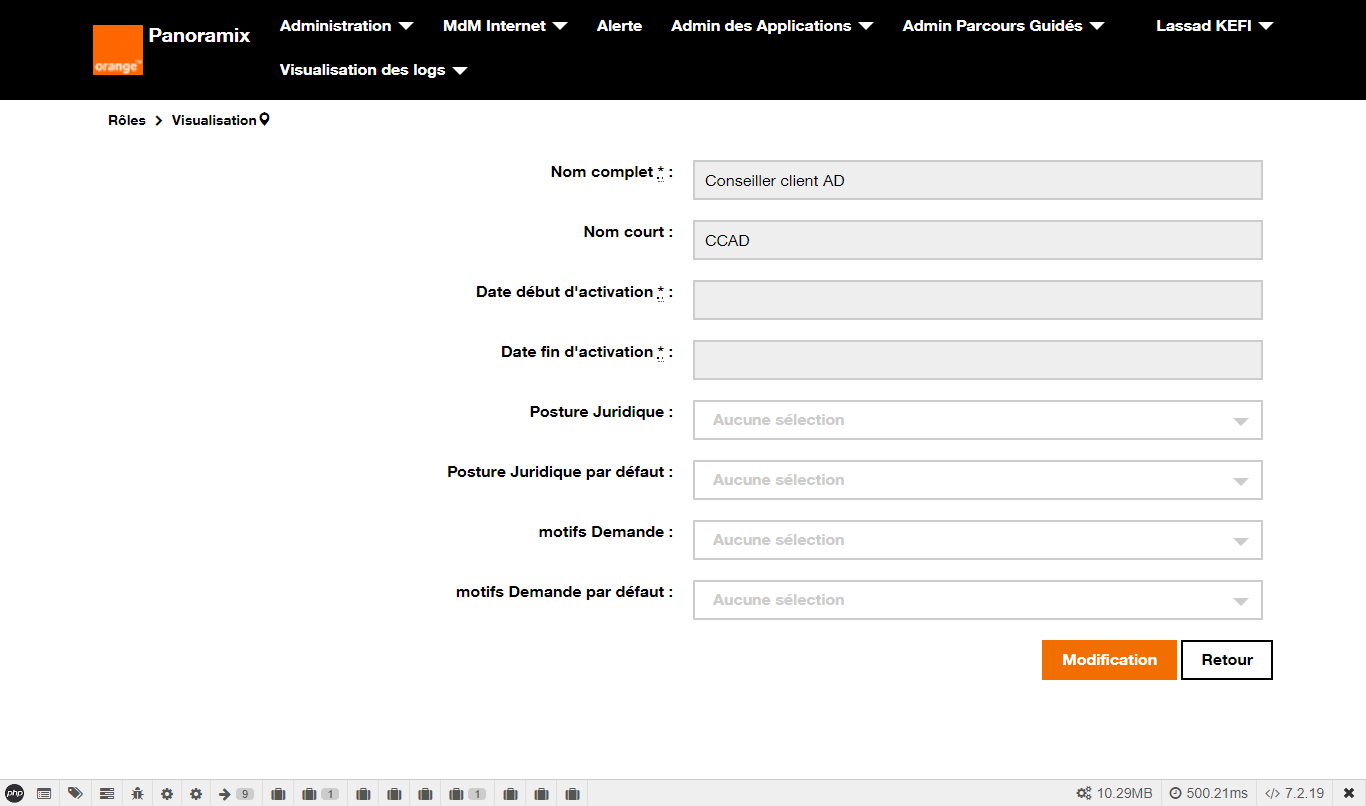
\includegraphics[width=0.6\linewidth]{img/screenshots/roles/view}
		\caption[Interface voir un rôle]{Interface consulter les données d'un rôle}
		\label{fig:view-role}
	\end{figure}
	\newpage
	\item Modifier ou créer un rôle
	\begin{figure}[H]
		\centering
		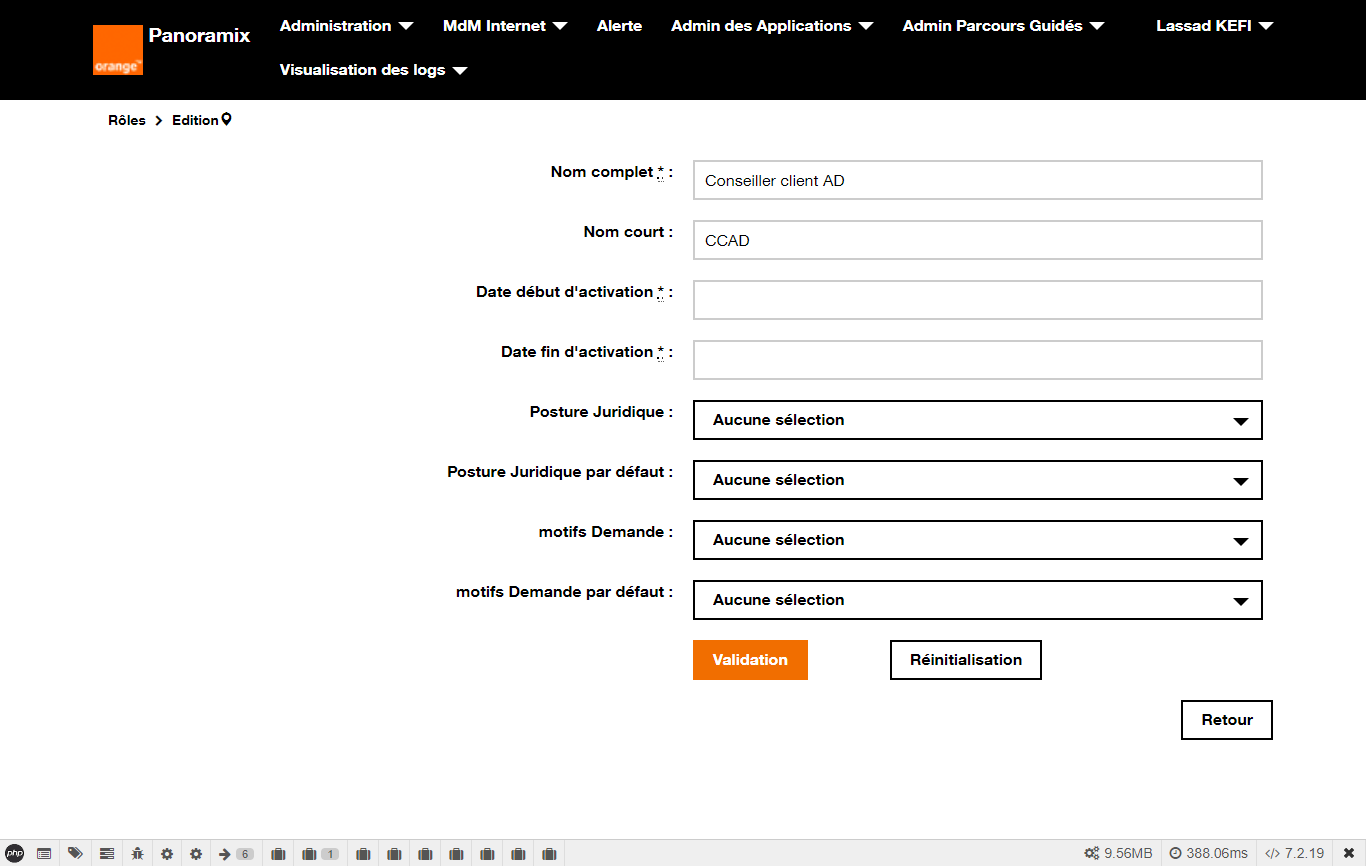
\includegraphics[width=0.7\linewidth]{img/screenshots/roles/edit}
		\caption[Interface modifier ou créer un rôle]{Interface modifier ou créer un rôle}
		\label{fig:modif-role}
	\end{figure}

	\item Supprimer un rôle
	\begin{figure}[H]
		\centering
		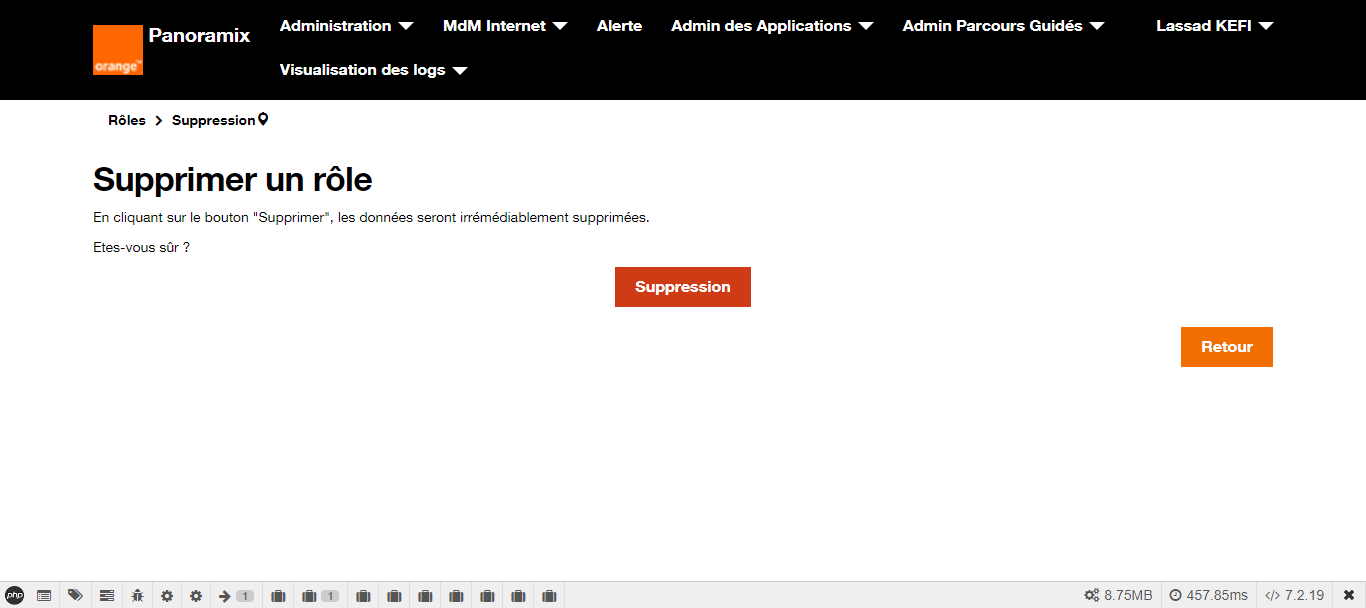
\includegraphics[width=0.7\linewidth]{img/screenshots/roles/delete}
		\caption[Interface sSupprimer un rôle]{Interface supprimer un rôle}
		\label{fig:delete-role}
	\end{figure}
\end{itemize}

\subsection{Interfaces de gestion des types de rôles}
les captures d'écran ci-dessous représentent les différentes IHM de gestion des types des rôles.
\newpage
\begin{itemize}
	\item Consultation des types de rôles et recherche
	\begin{figure}[H]
		\centering
		\includegraphics[width=0.8\linewidth]{"img/screenshots/type roles/index"}
		\caption[Interface consultation de types des rôles et recherche]{Interface consultation de types des rôles et recherche}
		\label{fig:index-tr}
	\end{figure}

	\item Consulter les types d'un rôle 
	\begin{figure}[H]
		\centering
		\includegraphics[width=0.8\linewidth]{"img/screenshots/type roles/view"}
		\caption[Interface voir les types d'un rôle]{Interface consulter les types d'un rôle}
		\label{fig:view-tr}
	\end{figure}
	\newpage
	\item Donner ou modifier des type à un rôle
	\begin{figure}[H]
		\centering
		\includegraphics[width=0.7\linewidth]{"img/screenshots/type roles/update"}
		\caption[Interface donner des type à un rôle]{Interface donner des type à un rôle}
		\label{fig:create-tr}
	\end{figure}
	
	\item Supprimer les type d'un rôle 
	\begin{figure}[H]
		\centering
		\includegraphics[width=0.7\linewidth]{"img/screenshots/type roles/delete"}
		\caption[Interface supprimer les type d'un rôle]{Interface supprimer les type d'un rôle}
		\label{fig:delete-tr}
	\end{figure}
\end{itemize}
\subsection{Interfaces de gestion des activations des rôles attribués à un utilisateurs}
les captures d'écran ci-dessous représentent les différentes IHM de des activations des rôles attribués à un utilisateurs.
\newpage
\begin{itemize}
	\item Consultation des activations et recherche
	\begin{figure}[H]
		\centering
		\includegraphics[width=0.7\linewidth]{"img/screenshots/activation des roles/index"}
		\caption[Interface consultation des activations des rôles aux utilisateurs]{Interface consultation des activations des rôles aux utilisateurs}
		\label{fig:index-activation}
	\end{figure}
	
	\item Consulter une activation de rôle d'un utilisateur
	\begin{figure}[H]
		\centering
		\includegraphics[width=0.7\linewidth]{"img/screenshots/activation des roles/view"}
		\caption[Interface voir une activation de rôle à un utilisateur]{Interface consulter une activation de rôle à un utilisateur}
		\label{fig:view-activation}
	\end{figure}
	\newpage
	\item Activer/désactiver un rôle d'un utilisateurs
	\begin{figure}[H]
		\centering
		\includegraphics[width=0.7\linewidth]{"img/screenshots/activation des roles/edit"}
		\caption[Interface activer/désactiver un rôle d'un utilisateurs]{Interface activer/désactiver un rôle d'un utilisateurs}
		\label{fig:create-activation}
	\end{figure}
\end{itemize}

\section*{Conclusion}
Au cours de ce chapitre, nous avons réalisé le deuxième sprint qui permet de développer le module «Gestion des utilisateurs » et le module «Gestion des rôles» en rédigeant sa conception et donc la “release 1” est terminée. Dans le chapitre suivant, nous entamons le développement du premier sprint de release 2. 

        \clearpage
        
        \chapter{Sprint 2 – Module Boutique}
	
\section*{Introduction}
Dans ce chapitre, nous allons nous intéresser à le module Boutique. Par la suite, nous nous intéresserons à l’aspect conceptuel et fonctionnel de ce sprint.

\section[Backlog sprint]{Backlog sprint}
Dans le backlog du sprint, nous présenterons deux parties :  le but du sprint et les user stories.

\subsection[But du sprint]{But du sprint}
En suivant le même principe que le sprint précédent, nous commencerons par définir l'objectif du sprint. Par conséquent, l'objectif de ce sprint est l'intégration de module Boutique et l’affectation des utilisateurs aux boutiques.
\subsection[User stories]{User stories}
Après avoir défini le but du sprint, nous pourrons lister les user stories qui appartiennent au sprint.
La table \ref{tab:user-stories-sprint-2} représente notre backlog de Sprint 2.
\begin{longtable}[c]{|l|l|l|}
	\hline
	\rowcolor[HTML]{C0C0C0} 
	User stories&
	Tâches &
	Complexité \\ \hline
	
	%
	\endhead
	%
	\begin{tabular}[c]{@{}l@{}}En tant qu’un administrateur, je\\ souhaite d’avoir toutes les \\ informations des boutiques à jour\end{tabular} &
	Intégrer le module Boutique dans le projet &
	1 \\ \hline
	\begin{tabular}[c]{@{}l@{}}En tant qu’un administrateur, je \\ souhaite d’affecter les utilisateurs\\ CPRO aux boutiques\end{tabular} &
	\begin{tabular}[c]{@{}l@{}}Ajouter les interfaces de la gestion\\ des affectations\\ \tabitem Consultation\\ \tabitem Modification\\ \tabitem Suppression\\ \tabitem Affectation des utilisateurs\\ \tabitem Recherche\\ et la logique derrière\end{tabular} &
	2 \\ \hline
	\begin{tabular}[c]{@{}l@{}}En tant qu’un administrateur, je\\ souhaite d’exporter les\\  affectations des utilisateurs CPRO\\  aux boutiques\end{tabular} &
	\begin{tabular}[c]{@{}l@{}}Ajouter bouton “exporter” dans\\ l’interface de gestion des\\ utilisateurs et la logique derrière\end{tabular} &
	3 \\ \hline
	\begin{tabular}[c]{@{}l@{}}En tant qu’un utilisateur de \\ Panoramix, je souhaite de simuler \\ la page SRCD\end{tabular} &
	Développer une interface SRCD &
	3 \\ \hline
	\captionsetup{justification=centering}
	\caption{User stories de sprint 2}
	\label{tab:user-stories-sprint-2}\\
\end{longtable}

\section{Etude de réalisation du sprint 2}
Cette section de notre projet présente les différents diagrammes de cas d’utilisation avec leurs raffinements
\newpage
\subsection{Diagramme de cas d’utilisation global sprint 2}
La figure \ref{fig:usecase-sprint2} décrit le diagramme de cas d’utilisation global du sprint 2
\begin{figure}[H]
	\centering
	\includegraphics[width=0.75\linewidth]{"img/conception/usecases/sprint 2/UseCase-sprint2"}
	\caption[Diagramme de cas d’utilisation global sprint 2]{Diagramme de cas d’utilisation global sprint 2}
	\label{fig:usecase-sprint2}
\end{figure}
\subsection{Raffinement et description textuelle des diagrammes de cas d’utilisation}
Dans cette section, nous présentons les diagrammes des cas d’utilisation détaillés et leurs descriptions textuelles.
\subsubsection{Description textuelle du cas d’utilisation «simulation SRCD»}
Le tableau \ref{tab:descrip-text-sim-srcd} contient la description textuelle du cas d’utilisation «simulation SRCD»

\begin{table}[H]
	\centering
	\begin{tabular}{|l|l|}
		\hline
		\rowcolor[HTML]{C0C0C0} 
		Cas d’utilisation & simulation SRCD                        \\ \hline
		Acteurs           & Toute personne ayant l’accès à la page \\ \hline
		Résumé &
		\begin{tabular}[c]{@{}l@{}}Semble à la page bouchon qui sert à simuler le \\ mécanisme que le client est inscrit en entrant à \\ la boutique\end{tabular} \\ \hline
		Scénario principal &
		\begin{tabular}[c]{@{}l@{}}L’utilisateur remplit le formulaire par :\\ code edo de la boutique\\ CUID du client \\ l'identifiant d'établissement\end{tabular} \\ \hline
		Post condition    & Le client sera ajouté au fil d’attente \\ \hline
	\end{tabular}
	\captionsetup{justification=centering}
	\caption{ Description textuelle du cas d’utilisation «simulation SRCD»}
	\label{tab:descrip-text-sim-srcd}
\end{table}

\subsubsection{Description textuelle du cas d’utilisation «consultation boutiques»}
Le tableau \ref{tab:descrip-text-consult-boutique} contient la description textuelle du cas d’utilisation «consultation boutiques»
\begin{table}[H]
	\centering
	\begin{tabular}{|l|l|}
		\hline
		\rowcolor[HTML]{C0C0C0} 
		Cas d’utilisation & consultation boutiques                 \\ \hline
		Acteurs           & Administrateur                         \\ \hline
		Résumé &
		\begin{tabular}[c]{@{}l@{}}L’administrateur peut consulter les données \\ boutique via l’interface\end{tabular} \\ \hline
		Précondition      & L’administrateur doit être authentifié \\ \hline
		Scénario principal &
		\begin{tabular}[c]{@{}l@{}}L’administrateur accède à la page des données \\ boutique, il peut faire une recherche et il peut voir \\ toutes informations concernant une boutique\end{tabular} \\ \hline
	\end{tabular}
	\captionsetup{justification=centering}
	\caption{Description textuelle du cas d’utilisation «consultation boutiques»}
	\label{tab:descrip-text-consult-boutique}
\end{table}
\newpage
\subsubsection{Cas d’utilisation «affectation  utilisateurs aux boutiques»}
La figure \ref{fig:usecase-affectation} illustre le raffinement du cas d’utilisation «affectation utilisateurs aux boutiques»
\begin{figure}[H]
	\centering
	\includegraphics[width=1\linewidth]{"img/conception/usecases/sprint 2/UseCase-affectation"}
	\caption[Diagramme cas d’utilisation «affectation utilisateurs aux boutiques»]{Cas d’utilisation «affectation utilisateurs aux boutiques»}
	\label{fig:usecase-affectation}
\end{figure}
\myparagraph{Description textuelle du cas d’utilisation «affectation  utilisateurs aux boutiques»}
Le tableau \ref{tab:descrip-text-affect-user-boutique} contient la description textuelle du cas d’utilisation «affectation utilisateurs aux boutiques»
\begin{table}[H]
	\centering
	\begin{tabular}{|l|l|}
		\hline
		\rowcolor[HTML]{C0C0C0} 
		Cas d’utilisation & Affectation utilisateurs aux boutiques                        \\ \hline
		Acteurs           & Administrateur                                                \\ \hline
		Résumé            & L’administrateur peut affecter des utilisateurs aux boutiques \\ \hline
		précondition &
		\begin{tabular}[c]{@{}l@{}}l’administrateur doit être authentifié\\ L’utilisateur doit être existant\\ La boutique doit être existante\end{tabular} \\ \hline
		Scénario principal &
		\begin{tabular}[c]{@{}l@{}}Pour gérer les affectations, l’administrateur peut :\\ affecter un utilisateur à une boutique\\ Modifier une affectation\\ Supprimer une affectation\\ Consulter les affectations\\ Rechercher des affectations\\Exporter les affectations en fichier CSV\end{tabular} \\ \hline
		Post condition    & Mettre à jour la liste des affectations                       \\ \hline
	\end{tabular}
	\captionsetup{justification=centering}
	\caption{Description textuelle du cas d’utilisation «affectation  utilisateurs aux boutiques»}
	\label{tab:descrip-text-affect-user-boutique}
\end{table}

\section{Conception}
Dans cette partie, nous présentons les différents diagrammes de classes ainsi que de séquence détaillés pour ce sprint.\newpage
\subsection{Diagramme de classes}
la figure \ref{fig:classdiag-sprint2} illustre la structure statique du sprint 2 schématisée dans un diagramme de classe globale.
Nous ajoutons 2 nouvelles classes :
\begin{itemize}
	\item \textbf{La classe Boutique :} représente les boutiques dans notre applications. Chaque boutique est identifiée par l'attribut code\_edo. Les autres champs sont expliquées dans le tableau \ref{tab:dictio-2} dans l'annexe à la page \pageref{tab:dictio-2}.
	\item \textbf{La classe associative Affectation : } permet aux utilisateurs d'appartenir à plusieurs boutiques.
\end{itemize}
\begin{figure}[H]
	\centering
	\includegraphics[width=0.5\linewidth]{img/conception/classes/ClassDiag-sprint2}
	\caption[Diagramme de classes de sprint 2]{Diagramme de classes de sprint 2}
	\label{fig:classdiag-sprint2}
\end{figure}

\subsection{Diagrammes de séquences détaillés}
Nous allons maintenant passer à l’aspect dynamique des opérations représentées dans le diagramme de classe à l’aide des diagrammes de séquences de système et d’objets.
\subsubsection[Quelques diagrammes de séquences système de Sprint 2]{Quelques diagrammes de séquences système de Sprint 2}
Dans cette section, nous présenterons quelques diagrammes de séquences système de “module Boutique” tels que : 
\myparagraph{Diagramme de séquences système d’«affecter un utilisateur au boutique»}
Après la consultation de page d'affectation, l'administrateur remplit la formulaire par le nom complet d'utilisateur, le CUID et le nom du boutique puis valide. Le système vérifie l'existence de l'utilisateur et la boutique et insère les données en ajoutant la date système de l'opération.\\
Un message de succès ou d'échec sera affiché.
\begin{figure}[H]
	\centering
	\includegraphics[width=0.7\linewidth]{"img/conception/sequences/sprint 2/affectation-system"}
	\caption[Diagramme de séquences système d’ «affecter un utilisateur au boutique»]{Diagramme de séquences système d’ «affecter un utilisateur au boutique»}
	\label{fig:affectation-system}
\end{figure}

\myparagraph{diagramme de séquences objets d’«affecter un utilisateur au boutique»}
Ce diagramme détaille de plus le diagramme précédent. Le service d'autocomplete assure une meilleure orientation sur la saisie des données.
\begin{figure}[H]
	\centering
	\includegraphics[width=0.65\linewidth]{"img/conception/sequences/sprint 2/affectation-obj"}
	\caption[diagramme de séquences objets d’ «affecter un utilisateur au boutique»]{diagramme de séquences objets d’ «affecter un utilisateur au boutique»}
	\label{fig:affectation-obj}
\end{figure}



\section{Réalisation}
Dans cette sections nous allons exposer les différentes interfaces réalisées dans le sprint 2. 
\subsection{Interfaces de consultation boutique}
les captures d'écran ci-dessous représentent les deux IHMs de consultation boutique.
\begin{itemize}
	\item Consultation des boutiques et recherche
	\begin{figure}[H]
		\centering
		\includegraphics[width=0.5\linewidth]{img/screenshots/boutique/index}
		\caption[Interface consultation des boutiques et recherche]{Interface consultation des boutiques et recherche}
		\label{fig:index-btq}
	\end{figure}
	
	\item Voir les données d'une boutique
	\begin{figure}[H]
		\centering
		\includegraphics[width=0.5\linewidth]{img/screenshots/boutique/view}
		\caption[Interfacevoir les données d'une boutique]{Interface voir les données d'une boutique}
		\label{fig:view-btq}
	\end{figure}
\end{itemize}

\subsection{Interfaces de gestion des affectations}
les captures d'écran ci-dessous représentent les différentes IHM de gestion des affectations.
\begin{itemize}
	\item Consultation des affectations et recherche
	\begin{figure}[H]
		\centering
		\includegraphics[width=0.6\linewidth]{"img/screenshots/affectation users-boutique/index"}
		\caption[Interface consultation des affectations et recherche]{Interface consultation des affectations et recherche}
		\label{fig:index-affectation}
	\end{figure}
	
	\item Consulter les données d'une affectation
	\begin{figure}[H]
		\centering
		\includegraphics[width=0.6\linewidth]{"img/screenshots/affectation users-boutique/view"}
		\caption[Interface voir une affectation]{Interface consulter les données d'une affectation}
		\label{fig:view-affectation}
	\end{figure}

	\item Affecter un utilisateur à une boutique
	\begin{figure}[H]
		\centering
		\includegraphics[width=0.6\linewidth]{"img/screenshots/affectation users-boutique/affectation"}
		\caption[Interface affecter un utilisateur à une boutique]{Interface affecter un utilisateur à une boutique}
		\label{fig:create-affectation}
	\end{figure}
	\newpage
	\item Résultat d'exportation des affectations
	\begin{figure}[H]
		\centering
		\includegraphics[width=0.7\linewidth]{"img/screenshots/affectation users-boutique/export"}
		\caption[Interface résultat d'exportation des affectations]{Interface résultat d'exportation des affectations}
		\label{fig:export-affectation}
	\end{figure}
\end{itemize}
\subsection{Interface de simulation SRCD}
la capture d'écran ci-dessous représente l’interface de simulation SRCD.
\begin{figure}[H]
	\centering
	\includegraphics[width=0.7\linewidth]{"img/screenshots/logs + srcd/screencapture-localhost-pano-pfe-panoramix-public-srcd-phtml-2020-06-11-18_18_04"}
	\caption[Interface de simulation SRCD]{Interface de simulation SRCD}
	\label{fig:srcd}
\end{figure}

\section*{Conclusion}
Dans ce chapitre, nous avons terminé le troisième sprint, qui a permis l'intégration de “module Boutique” et la gestion des affectations en rédigeant sa conception. Dans le chapitre suivant, nous commençons le sprint final de notre projet.

        \clearpage
        
        \chapter{Sprint 3 – Gestion des PEF}
	
\section*{Introduction}
Dans ce chapitre nous allons principalement nous intéresser à la fonctionnalité la plus  importante de notre projet. Tout comme le sprint précédent, nous procéderons par étapes afin d’éviter d’ignorer une partie de ce sprint.

\section{Backlog sprint}
Dans le backlog du sprint, nous présenterons deux parties suivantes
\subsection{But de sprint}
Le but de ce sprint est de gérer les PEF pour que chaque utilisateur peut les accéder lors l’ouverture de fiche client.
\subsection{User stories}
Après avoir défini l'objectif du sprint, nous pouvons lister les user stories qui appartiennent au sprint.
Le tableau \ref{tab:user-stories-sprint3} liste les différents user stories de notre sprint :
\begin{longtable}[c]{|l|l|l|}
	\hline
	\rowcolor[HTML]{C0C0C0} 
	User stories &
	Tâches &
	complexité \\ \hline
	\endhead
	%
	\begin{tabular}[c]{@{}l@{}}En tant qu’un administrateur, je\\ souhaite de gérer les catégories \\ des PEF\end{tabular} &
	\begin{tabular}[c]{@{}l@{}}Djouter les interfaces de la gestion\\ des catégories des PEF :\\ \tabitem Consultation\\ \tabitem Ajout\\ \tabitem Modification\\ \tabitem Suppression\\ \tabitem Recherche\\ et la logique derrière\end{tabular} &
	2 \\ \hline
	\begin{tabular}[c]{@{}l@{}}En tant qu’un administrateur, je\\ souhaite de gérer les types\\ des catégories des PEF\end{tabular} &
	\begin{tabular}[c]{@{}l@{}}Ajouter les interfaces de la gestion\\ des types de catégories :\\ \tabitem Consultation\\ \tabitem Ajout\\ \tabitem Modification\\ \tabitem Suppression\\ \tabitem Recherche\\ et la logique derrière\end{tabular} &
	2 \\ \hline
	\begin{tabular}[c]{@{}l@{}}En tant qu’un administrateur, je\\ souhaite de gérer les PEF\end{tabular} &
	\begin{tabular}[c]{@{}l@{}}Ajouter les interfaces de la gestion\\ des PEF :\\ \tabitem Consultation\\ \tabitem Ajout\\ \tabitem Modification\\ \tabitem Suppression\\ \tabitem Recherche\\ et la logique derrière\end{tabular} &
	2 \\ \hline
	\begin{tabular}[c]{@{}l@{}}En tant qu’un administrateur, je\\ souhaite de consulter les types \\ des PEF\end{tabular} &
	\begin{tabular}[c]{@{}l@{}}Ajouter les interfaces de consultation \\ des types des PEF :\\ \tabitem Consultation \\ \tabitem Recherche\\ et la logique derrière\end{tabular} &
	3 \\ \hline
	\begin{tabular}[c]{@{}l@{}}En tant qu’un administrateur, je\\ souhaite de gérer la visibilité \\ des PEF au boutique\end{tabular} &
	\begin{tabular}[c]{@{}l@{}}Ajouter les interfaces de la gestion\\ de visibilité des PEF :\\ \tabitem Consultation\\ \tabitem Ajout\\ \tabitem Modification\\ \tabitem Suppression\\ \tabitem Recherche\\ et la logique derrière\end{tabular} &
	1 \\ \hline
	\begin{tabular}[c]{@{}l@{}}En tant qu’un conseiller client réactif, je\\ souhaite de consulter les PEF \\ disponibles lors l’ouverture de\\ fiche client\end{tabular} &
	\begin{tabular}[c]{@{}l@{}}Fournir la liste des PEF au \\ conseiller client réactif en fonction \\ de type de l’utilisateur ( CPRO \\ pour boutique ou 3901 pour \\ centre d’appel) de catégorie et de\\  type de catégorie\end{tabular} &
	1 \\ \hline
	\begin{tabular}[c]{@{}l@{}}En tant qu’un administrateur, je\\ souhaite d’avoir une vue totale \\ des logs des APIs\end{tabular} &
	\begin{tabular}[c]{@{}l@{}}Développer une interface qui \\ comporte les informations \\ complètes de logs APIs\end{tabular} &
	2 \\ \hline
	\begin{tabular}[c]{@{}l@{}}En tant qu’un administrateur, je\\ souhaite de tracer toutes actions\\ prises par les utilisateurs sur\\ l’application\end{tabular} &
	\begin{tabular}[c]{@{}l@{}}Elaborer les logs de navigation sur \\ l’application et les actions prises\end{tabular} &
	3 \\ \hline
	\captionsetup{justification=centering}
	\caption{User stories de sprint 3}
	\label{tab:user-stories-sprint3}\\
\end{longtable}

\section{Etude de réalisation du sprint 3}
Cette section de notre projet présente les différents diagrammes de cas d’utilisation avec leurs raffinements.
\subsection{Diagramme de cas d’utilisation global sprint 3}
La figure \ref{fig:usecase-sprint3} décrit le diagramme de cas d’utilisation global du sprint 3.
\begin{figure}[H]
	\centering
	\includegraphics[width=0.58\linewidth]{"img/conception/usecases/sprint 3/UseCase-sprint3"}
	\caption[Diagramme de cas d’utilisation global sprint 3]{Diagramme de cas d’utilisation global sprint 3}
	\label{fig:usecase-sprint3}
\end{figure}

\subsection{Raffinement et description textuelle des diagrammes de cas d’utilisation}
Dans cette section, nous présentons les diagrammes des cas d’utilisation détaillés et leurs descriptions textuelles.
\subsubsection{Cas d’utilisation «gestion des catégories»}
La figure \ref{fig:usecase-gestion-categories} illustre le raffinement du cas d’utilisation « gestion des catégories »

\begin{figure}[H]
	\centering
	\includegraphics[width=0.7\linewidth]{"img/conception/usecases/sprint 3/usecase-gestion-categories"}
	\caption[Cas d’utilisation «gestion des catégories»]{Gas d’utilisation «gestion des catégories»}
	\label{fig:usecase-gestion-categories}
\end{figure}

\myparagraph{Description textuelle du cas d’utilisation «gestion des catégories»}
Le tableau \ref{tab:descrip-text-gestion-cat} contient la description textuelle du cas d’utilisation «gestion des catégories»
\begin{table}[H]
	\centering
	\begin{tabular}{|l|l|}
		\hline
		\rowcolor[HTML]{C0C0C0} 
		Cas d’utilisation & Gestion des catégories                     \\ \hline
		Acteur            & Administrateur                             \\ \hline
		Résumé            & L’administrateur peut gérer les catégories \\ \hline
		Précondition      & L’administrateur doit être authentifié     \\ \hline
		Scénario principal &
		\begin{tabular}[c]{@{}l@{}}Pour gérer les catégories, l’administrateur peut :\\ Ajouter une catégorie\\ Modifier une catégorie ou les types d'une catégorie\\ Supprimer une catégorie\\ Consulter les catégories\\ Rechercher des catégories\end{tabular} \\ \hline
		Post condition    & Mettre à jour la liste des catégories      \\ \hline
	\end{tabular}
	\captionsetup{justification=centering}
	\caption{Description textuelle du cas d’utilisation «gestion des catégories»}
	\label{tab:descrip-text-gestion-cat}
\end{table}
\subsubsection{Cas d’utilisation «gestion des PEF»}
La figure \ref{fig:usecase-gestion-pef} illustre le raffinement du cas d’utilisation «gestion des PEF»
\begin{figure}[H]
	\centering
	\includegraphics[width=1\linewidth]{"img/conception/usecases/sprint 3/usecase-gestion-PEF"}
	\caption[Cas d’utilisation «gestion des PEF»]{Cas d’utilisation «gestion des PEF»}
	\label{fig:usecase-gestion-pef}
\end{figure}
\myparagraph{Description textuelle du cas d’utilisation «gestion des PEF»}
Le tableau \ref{tab:descrip-text-gestion-pef} contient la description textuelle du ccas d’utilisation «gestion des PEF».
\begin{table}[H]
	\centering
	\begin{tabular}{|l|l|}
		\hline
		\rowcolor[HTML]{C0C0C0} 
		Cas d’utilisation & Gestion des PEF                        \\ \hline
		Acteur            & Administrateur                         \\ \hline
		Résumé            & L’administrateur peut gérer les PEF    \\ \hline
		Précondition      & L’administrateur doit être authentifié \\ \hline
		Scénario principal &
		\begin{tabular}[c]{@{}l@{}}Pour gérer les PEF , l’administrateur peut :\\ Ajouter un PEF \\ Modifier un PEF \\ Supprimer un PEF \\ Consulter les PEF \\ Rechercher des PEF\end{tabular} \\ \hline
		Post condition    & Mettre à jour la liste des PEF         \\ \hline
	\end{tabular}
\captionsetup{justification=centering}
	\caption{Description textuelle du cas d’utilisation «gestion des PEF»}
	\label{tab:descrip-text-gestion-pef}
\end{table}

\subsubsection{Cas d’utilisation «visibilité des PEF au boutique»}
La figure \ref{fig:usecase-gestion-visibilite} illustre le raffinement du cas d’utilisation «gestion des PEF»

\begin{figure}[H]
	\centering
	\includegraphics[width=1\linewidth]{"img/conception/usecases/sprint 3/usecase-gestion-visibilite"}
	\caption[Cas d’utilisation «visibilité des PEF au boutique»]{Cas d’utilisation «visibilité des PEF au boutique»}
	\label{fig:usecase-gestion-visibilite}
\end{figure}

\myparagraph{Description textuelle du cas d’utilisation «visibilité des PEF au boutique»}
Le tableau \ref{tab:descrip-text-visib} contient la description textuelle du cas d’utilisation «visibilité des PEF au boutique»

\begin{table}[H]
	\centering
	\begin{tabular}{|l|l|}
		\hline
		\rowcolor[HTML]{C0C0C0} 
		Cas d’utilisation & Visibilité des PEF au boutique                                                  \\ \hline
		Acteur            & Administrateur                                                                  \\ \hline
		Résumé            & L’administrateur peut donner l’autorité à une boutique pour utiliser un tel PEF \\ \hline
		Précondition &
		\begin{tabular}[c]{@{}l@{}}l’administrateur doit être authentifié\\ La boutique doit être existante\\ Le PEF doit être existant\end{tabular} \\ \hline
		Scénario principal &
		\begin{tabular}[c]{@{}l@{}}Pour gérer la visibilité , l’administrateur peut :\\ ajouter un PEF à une boutique\\ Modifier la visibilité de boutique\\ limiter la visibilité de boutique\\ Consulter les visibilités des boutiques\\ Rechercher des visibilités boutiques\end{tabular} \\ \hline
		Post condition    & Mettre à jour la liste des visibilités                                          \\ \hline
	\end{tabular}
	\captionsetup{justification=centering}
	\caption{Description textuelle du cas d’utilisation «visibilité des PEF au boutique»}
	\label{tab:descrip-text-visib}
\end{table}

\subsubsection{Description textuelle du cas d’utilisation «consultation fiche client»}
Le tableau \ref{tab:descrip-text-fiche-client} contient la description textuelle du cas d’utilisation «consultation fiche client»
\begin{table}[H]
	\centering
	\begin{tabular}{|l|l|}
		\hline
		\rowcolor[HTML]{C0C0C0} 
		Cas d’utilisation & Consultation fiche client                                                                        \\ \hline
		Acteur            & Le conseiller client réactif et l’administrateur                                                 \\ \hline
		Résumé &
		\begin{tabular}[c]{@{}l@{}}Les acteurs auront une liste des PEF classés selon\\ leur catégorie en fonction de type d’utilisateur, type\\ des catégories\end{tabular} \\ \hline
		Précondition      & \begin{tabular}[c]{@{}l@{}}L’acteur doit être authentifié\\ Ouvrir une fiche client\end{tabular} \\ \hline
		Scénario principal &
		\begin{tabular}[c]{@{}l@{}}Pour consulter les PEF, l’acteur doit ouvrir\\ une fiche client. Puis un menu sera affiché\\ contenant la liste des applications.\\ Cette dernière contient les PEF classés selon\\ leurs catégories.\end{tabular} \\ \hline
	\end{tabular}
	\captionsetup{justification=centering}
	\caption{Description textuelle du cas d’utilisation «consultation fiche client»}
	\label{tab:descrip-text-fiche-client}
\end{table}

\subsubsection{Description textuelle du cas d’utilisation «consultation des logs API»}
Le tableau \ref{tab:descrip-text-api-logs} contient la description textuelle du cas d’utilisation «consultation des logs API»

\begin{table}[H]
	\centering
	\begin{tabular}{|l|l|}
		\hline
		\rowcolor[HTML]{C0C0C0} 
		Cas d’utilisation & consultation des logs API                                                                                                 \\ \hline
		Acteur            & administrateur                                                                                                            \\ \hline
		Résumé            & L’administrateur peut consulter les logs des APIs                                                                         \\ \hline
		précondition      & \begin{tabular}[c]{@{}l@{}}l’administrateur doit être authentifié\\ Les fichiers logs doivent être existants\end{tabular} \\ \hline
		scénario principal &
		\begin{tabular}[c]{@{}l@{}}Pour consultation des logs API , l’administrateur\\ va consulter le tableau des statistiques des logs.\\ Si l’administrateur souhaite d’avoir des informations\\ détaillées, il peut cliquer sur la colonne de table \\ et un modal sera affiché contenant toutes les détails\end{tabular} \\ \hline
	\end{tabular}
	\captionsetup{justification=centering}
	\caption{Description textuelle du cas d’utilisation «consultation des logs API»}
	\label{tab:descrip-text-api-logs}
\end{table}

\subsubsection{Description textuelle du cas d’utilisation «élaboration des logs Panoramix»}
Le tableau \ref{tab:descrip-text-elab-logs} contient la description textuelle du cas d’utilisation «élaboration des logs Panoramix»

\begin{longtable}[c]{|l|l|}
	\hline
	\rowcolor[HTML]{C0C0C0} 
	Cas d’utilisation & Elaboration des logs Panoramix                                                                                                                         \\ \hline
	\endfirsthead
	%
	\endhead
	%
	Acteur            & Système                                                                                                                                                \\ \hline
	Résumé            & \begin{tabular}[c]{@{}l@{}}Après chaque action prise par les utilisateurs,\\ le système doit écrire dans le log cette action\\ en détails\end{tabular} \\ \hline
	Précondition      & Une action est prise par un utilisateur                                                                                                                \\ \hline
	Scénario principal &
	\begin{tabular}[c]{@{}l@{}}Chaque navigation ou action prise sur Panoramix,\\ le système doit décrire cette action sous un tel\\ format  structuré qui comporte\\ les informations suivante :\\ \tabitem Date d’action\\ \tabitem Heure d’action\\ \tabitem CUID d’utilisateur\\ \tabitem Nom d’utilisateur\\ \tabitem Prénom de l’utilisateur\\ \tabitem Sujet d’action\\ \tabitem L’action\\ \tabitem Etat d’action\\ \tabitem Rôle d’utilisateur\\ \tabitem Département d’utilisateur \\ \tabitem etc..\\ Ces champs doivent être séparés par une “;”\end{tabular} \\ \hline
	Post condition    & Le fichier log sera rédigé                                                                                                                             \\ \hline
	\caption{Description textuelle du cas d’utilisation «élaboration des logs Panoramix»}
	\label{tab:descrip-text-elab-logs}\\
\end{longtable}

\section{Conception}
Dans cette partie, nous présentons les différents diagrammes de classes ainsi que de séquence détaillés pour ce sprint. \newpage
\subsection{Diagramme de classes}
la figure \ref{fig:classdiag-sprint3} illustre la structure statique du sprint 3 schématisé dans un diagramme de classe globale.
\begin{figure}[H]
	\centering
	\includegraphics[width=0.7\linewidth]{img/conception/classes/ClassDiag-sprint3}
	\caption[Diagramme de classes sprint 3]{Diagramme de classes sprint 3}
	\label{fig:classdiag-sprint3}
\end{figure}

\subsection{Diagrammes de séquences détaillés}
Nous allons maintenant passer à l’aspect dynamique des opérations représentées dans le diagramme de classe à l’aide des diagrammes de séquences de système et d’objets.
\subsubsection{Quelques diagramme de séquences système de Sprint 3}
Dans cette section, nous présenterons quelques diagrammes de séquences système de «gestion des PEF» tels que : \newpage

\myparagraph{Diagramme de séquences système de «visibilité des PEF au boutique»} 
	\begin{figure}[H]
		\centering
		\includegraphics[width=0.7\linewidth]{"img/conception/sequences/sprint 3/visibilite-system"}
		\caption[Diagramme de séquences système de «visibilité des PEF au boutique»]{Diagramme de séquences système de «visibilité des PEF au boutique»}
		\label{fig:visibilite-system}
	\end{figure}


\subsubsection{Quelques diagramme de séquences objets de Sprint 3}
Nous présentons dans ce qui suit quelques diagrammes de séquences objets détaillés \\du sprint 3.
\myparagraph{Diagramme de séquences d’objets de «consultation logs API»} 
	\begin{figure}[H]
		\centering
		\includegraphics[width=0.7\linewidth]{"img/conception/sequences/sprint 3/log-api-obj"}
		\caption[Diagramme de séquences d’objets de «consultation logs API»]{Diagramme de séquences d’objets de «consultation logs API»}
		\label{fig:log-api-obj}
	\end{figure}
	\newpage
\myparagraph{Diagramme de séquences d’objets de «fiche client»} 
	\begin{figure}[H]
		\centering
		\includegraphics[width=0.7\linewidth]{"img/conception/sequences/sprint 3/fiche-client-obj"}
		\caption[Diagramme de séquences d’objets de «fiche client»]{Diagramme de séquences d’objets de «fiche client»}
		\label{fig:fiche-client-obj}
	\end{figure}

\section{Réalisation}
Dans cette section, nous allons exposer les différentes interfaces réalisées dans le sprint 3.
\subsection{Interfaces de gestion des catégories}
\begin{itemize}
	\item Consultation des catégories et recherche
	\begin{figure}[H]
		\centering
		\includegraphics[width=0.5\linewidth]{img/screenshots/categorie/index}
		\caption[Interface consultation des catégories et recherche]{Interface consultation des catégories et recherche}
		\label{fig:index-categorie}
	\end{figure}
	
	\item Modifier ou créer une catégories
	\begin{figure}[H]
		\centering
		\includegraphics[width=0.6\linewidth]{img/screenshots/categorie/create-edit}
		\caption[Interface modifier une catégorie]{Interface modifier une catégorie}
		\label{fig:edit-categorie}
	\end{figure}

	\item Supprimer une catégories
	\begin{figure}[H]
		\centering
		\includegraphics[width=0.6\linewidth]{img/screenshots/categorie/delete}
		\caption[Interface supprimer une catégorie]{Interface supprimer une catégorie}
		\label{fig:delete-categorie}
	\end{figure}
\end{itemize}

\subsection{Interfaces de gestion des type de catégories}

\begin{itemize}
	\item Consultation des types des catégories
	\begin{figure}[H]
		\centering
		\includegraphics[width=0.6\linewidth]{img/screenshots/categorie-type/index}
		\caption[Interface consultation des types des catégories]{Interface consultation des types des catégories}
		\label{fig:index-tc}
	\end{figure}
	\newpage
	\item Voir un type des catégories
	\begin{figure}[H]
		\centering
		\includegraphics[width=0.7\linewidth]{img/screenshots/categorie-type/view}
		\caption[Interface voir un type des catégories]{Interface voir un type des catégories}
		\label{fig:view-tc}
	\end{figure}
	
	\item Modifier ou créer un type des catégories
	\begin{figure}[H]
		\centering
		\includegraphics[width=0.7\linewidth]{img/screenshots/categorie-type/create-edit}
		\caption[Interface modifier un type des catégories]{Interface modifier un type des catégories}
		\label{fig:edit-tc}
	\end{figure}

	\item Supprimer un type des catégories
	\begin{figure}[H]
		\centering
		\includegraphics[width=0.7\linewidth]{img/screenshots/categorie-type/delete}
		\caption[Interface supprimer un type des catégories]{Interface supprimer un type des catégories}
		\label{fig:delete-tc}
	\end{figure}
\end{itemize}
\newpage
\subsection{Interfaces de gestion des PEF}
\begin{itemize}
	\item Consultation des PEF et recherche
	\begin{figure}[H]
		\centering
		\includegraphics[width=0.55\linewidth]{img/screenshots/pef/index}
		\caption[Interface consultation des PEF et recherche]{Interface consultation des PEF et recherche}
		\label{fig:index-pef}
	\end{figure}

	\item Voir les données d'un PEF
	\begin{figure}[H]
		\centering
		\includegraphics[width=0.55\linewidth]{img/screenshots/pef/view}
		\caption[Interface voir les données d'un PEF]{Interface voir les données d'un PEF}
		\label{fig:view-pef}
	\end{figure}
	
	\item Modifier ou créer un PEF
	\begin{figure}[H]
		\centering
		\includegraphics[width=0.7\linewidth]{img/screenshots/pef/edit}
		\caption[Interface modifier ou créer un PEF]{Interface modifier ou créer un PEF}
		\label{fig:create-pef}
	\end{figure}
	
	\item Supprimer un PEF
	\begin{figure}[H]
		\centering
		\includegraphics[width=0.7\linewidth]{img/screenshots/pef/delete}
		\caption[Interface supprimer un PEF]{Interface supprimer un PEF}
		\label{fig:delete-pef}
	\end{figure}
\end{itemize}
\newpage
\subsection{Interfaces de consultation des types de PEF}
\begin{itemize}
	\item Consultation des types de PEF et recherche
	\begin{figure}[H]
		\centering
		\includegraphics[width=0.5\linewidth]{img/screenshots/pef-type/index}
		\caption[Interface consultation des types de PEF et recherche]{Interface consultation des types de PEF et recherche}
		\label{fig:index-tp}
	\end{figure}
	
	\item Voir un type de PEF 
	\begin{figure}[H]
		\centering
		\includegraphics[width=0.5\linewidth]{img/screenshots/pef-type/view}
		\caption[Interface voir un type de PEF ]{Interface voir un type de PEF }
		\label{fig:view-tp}
	\end{figure}
\end{itemize}

\subsection{Interfaces de visibilité des PEF aux boutiques}
\begin{itemize}
	\item Consultation des visibilités et recherche
	\begin{figure}[H]
		\centering
		\includegraphics[width=0.5\linewidth]{"img/screenshots/visibilité pef-boutique/index"}
		\caption[Interface consultation des visibilités et recherche]{Interface consultation des visibilités et recherche}
		\label{fig:index-visib}
	\end{figure}
	
	\item Voir une visibilité 
	\begin{figure}[H]
		\centering
		\includegraphics[width=0.5\linewidth]{"img/screenshots/visibilité pef-boutique/view"}
		\caption[Interface voir une visibilité]{Interface voir une visibilité }
		\label{fig:view-visib}
	\end{figure}

	\item Modifier ou créer une visibilité 
	\begin{figure}[H]
		\centering
		\includegraphics[width=0.5\linewidth]{"img/screenshots/visibilité pef-boutique/view"}
		\caption[Interface modifier ou créer une visibilité]{Interface modifier ou créer une visibilité}
		\label{fig:edit-visib}
	\end{figure}

	\item Supprimer une visibilité 
	\begin{figure}[H]
		\centering
		\includegraphics[width=0.5\linewidth]{"img/screenshots/visibilité pef-boutique/view"}
		\caption[Interface supprimer une visibilité]{Interface supprimer une visibilité}
		\label{fig:delete-visib}
	\end{figure}
	
\end{itemize}
\subsection{Interfaces de consultation des PEF au fiche client}
\begin{figure}[H]
	\centering
	\includegraphics[width=0.5\linewidth]{"img/screenshots/fiche client/fiche client et accès au pef"}
	\caption[Interface de consultation des PEF au fiche client]{Interface de consultation des PEF au fiche client}
	\label{fig:fiche-client-et-acces-au-pef}
\end{figure}

\subsection{Interface de consultation des log API}
\begin{figure}[H]
	\centering
	\includegraphics[width=0.7\linewidth]{"img/screenshots/logs + srcd/detailed log"}
	\caption[Interface de consultation des log API]{Interface de consultation des log API}
	\label{fig:detailed-log}
\end{figure}

\subsection{Capture de fichier de logs d’application Panoramix}

\begin{figure}[H]
	\centering
	\includegraphics[width=0.7\linewidth]{"img/screenshots/logs + srcd/log-application"}
	\caption[Capture de fichier de logs d’application Panoramix]{Capture de fichier de logs d’application Panoramix}
	\label{fig:log-application}
\end{figure}

\section*{Conclusion}
Dans ce chapitre, nous avons terminé le dernier sprint de notre application Panoramix et donc nous avons terminé le dernier release en traitant les détails de la réalisation de notre sprint et en montrant les différentes interfaces de notre application.







        \clearpage
        
        \chapter*{Conclusion générale}
\addcontentsline{toc}{chapter}{Conclusion générale}
\markboth{Conclusion générale}{}

Ce stage, a été, sous plusieurs aspects riches d'enseignements, nous avons commencé dans un premier lieu par comprendre le contexte général de notre application et identifier les différents besoins de notre futur système. Nous avons préparé par la suite notre planning de travail en respectant les priorités de nos besoins suite à une discussion entre l'équipe. Ce projet de fin d'études a été réalisé au sein de la société Sofrecom Tunisie. Il consiste à la refonte l'application web Panoramix qui assure l'interaction entre les clients PRO PME et les conseillers réactifs.\\\newline

Le présent manuscrit détaille toutes les étapes par lesquelles nous sommes passées pour arriver au résultat attendu. Nous avons essayé tout au long de notre travail de construire notre application incrément par incrément en utilisant la méthodologie Scrum.\\\newline

Ce travail nous a été très instructif de point de vue des connaissances acquises. Il nous a procuré une opportunité pour, d'une part aborder un domaine métier et d'autre part confirmer une fois de plus nos connaissances dans le développement PHP ou les tests de non régression et toucher de près plusieurs aspects du cycle de vie d'un produit logiciel.\\\newline

Par ailleurs, d'un point de vue technologique, le projet a été très enrichissant puisqu'il nous a donné l'occasion d'étudier et d'utiliser une panoplie de technologies (Jenkins, Robot Framework, OFT, ...).\\\newline

Hormis le côté technique, ce projet a été une opportunité pour appréhender le travail dans une hiérarchie professionnelle au sein d'une grande société et, les difficultés inhérentes comme la répartition du temps et des efforts. En ainsi que les bonnes pratiques nécessaires à la réalisation d'un produit de qualité.Aussi au cours de ce stage, nous avons participé à plusieurs événements et ateliers organisés
par la société SOFRECOM malgré la situation difficile que nous avions vécue. Pour conclure, nous estimons avoir satisfait les objectifs initialement fixés, à savoir la refonte l'application web Panoramix d'Orange France.\\\newline

Ce travail a accompli ses objectifs, mais comme toute œuvre humaine il ne prétend pas la perfection et nécessite alors des améliorations. Dans cette optique, l'application peut être amélioré en changeant la solution actuelle en des micro-services. En plus, il sera toujours intéressant d'ajouter un module pour superviser les composants de système et les composants matériels en temps réel.\\
        \clearpage
        
        % @author: Stoufa
		% the command `\nocite{*}` is mandatory to avoid the “no \citation commands” error
        % https://tex.stackexchange.com/questions/18045/problem-with-compiling-bibtex-no-citation-commands-error
        %\nocite{*}
        \printbibliography[heading=bibintoc]
        
        \chapter*{Annexes}
\addcontentsline{toc}{chapter}{Annexes}
\markboth{Annexes}{}
\stepcounter{chapter}
\addtocontents{lot}{\vspace{3.8mm}}
\addtocontents{lof}{\vspace{3.8mm}}

%Mettez vos annexes ici...

%===================== ANNEXE 1 =====================%
\section*{Annexe 1.~L'algorigramme de «mise à jour des données boutiques»}
\addcontentsline{toc}{section}{Annexe 1.~Exemple d'annexe}
Ce diagramme représente l'algorithme de script bash qui s'exécute quotidiennement pour mettre à jour les données boutiques.
\begin{figure}[H]
	\centering
	\includegraphics[width=0.5\linewidth]{img/conception/FlowchartDiagram-update-boutique}
	\caption[L'algorigramme de «mise à jour des données boutiques»]{L'algorigramme de «mise à jour des données boutiques»}
	\label{fig:flowchartdiagram-update-boutique}
\end{figure}
\newpage
%===================== ANNEXE 2 =====================%
\section*{Annexe 2.~Entreprise}
\addcontentsline{toc}{section}{Annexe 2.~Entreprise}

\addcontentsline{lof}{figure}{Annexe 2.1~~~Logo d'entreprise}

La figure annexe 2.1 présente le logo entreprise.
\begin{figure}[htpb]
    \centering
    \frame{\includegraphics[width=0.45\columnwidth]{Logo_Entreprise}}
    {\\\textbf{Figure annexe 2.1:} Logo d'entreprise}
\end{figure}


        \clearpage

    \backmatter
        %===== File containing the back cover of the document =====%
%                                                          %
% Copyright (C) ISI - All Rights Reserved                  %
% Proprietary                                              %
% Written by Med Hossam <med.hossam@gmail.com>, April 2016 %
%                                                          %
% @author: HEDHILI Med Houssemeddine                       %
% @linkedin: http://tn.linkedin.com/in/medhossam           %
%==========================================================%

%== It's advised to not modify the content of this file ===%
% To set your information, go to global_config.tex file    %
%==========================================================%

\thispagestyle{backcover}
\newgeometry{bottom=25mm,left=15mm,top=20mm,right=15mm}

\begin{changemargin}{3mm}{0cm}
    \begin{minipage}[c]{0.96\columnwidth}
        \vspace{3cm}
        \selectlanguage{arabic}
        \noindent\rule{17.3cm}{0.4pt}
        {\LARGE\textbf{ملخّص}}
        \vskip1mm
            \begingroup
                \small
                \@arabicAbstract
            \endgroup
        \vskip1mm
        {\textbf{كلمات مفاتيح : } 
            \begingroup
                \@arabicAbstractKeywords
            \endgroup
        }
        
        {\ifthenelse{\boolean{wantToTypeCompanyAddress}}
        {% IF TRUE
            \vskip5mm
        }{\vskip8mm}}
    	\vspace{3cm}
        \noindent\rule{17.3cm}{0.4pt}
        
        \selectlanguage{french}
        
        {\LARGE\textbf{Résumé}}
        \vskip1mm
            \begingroup
                \large
                \@frenchAbstract
            \endgroup
        \vskip1mm
        {\textbf{Mots clés : }
            \begingroup
                \@frenchAbstractKeywords
            \endgroup
        }
        
        {\ifthenelse{\boolean{wantToTypeCompanyAddress}}
        {% IF TRUE
            \vskip5mm
        }{\vskip8mm}}
    \vspace{3cm}
        \noindent\rule{17.3cm}{0.4pt}
        
        \selectlanguage{english}
        {\LARGE\textbf{Abstract}}
        \vskip1mm
            \begingroup
                \large
                \@englishAbstract
            \endgroup
        \vskip1mm
        {\textbf{Keywords : }
            \begingroup
                \@englishAbstractKeywords
            \endgroup
        }
   
    \end{minipage}
    
\end{changemargin}
    
\end{document}